\def\PrintEdition{1}% bookstyle.tex -- the designed edition of The Price of Agency ("the ledger rule").
% White pages. A single blue rule in the left column runs beside the machinery (theorems, mathematics, models);
% a double brass rule beside the receipts (code, records); a dashed grey rule beside the one fenced conjecture.
% Built by design/build_book.py from the markdown manuscript; nothing here contains manuscript text.
% Two editions from this one file. The screen edition (book.pdf) is one-sided. The print edition (book_print.pdf, built with
% `build_book.py --print`, which defines \PrintEdition) is two-sided: the text block moves away from the spine, chapters and
% parts open on right-hand pages, folios and the edge strips sit on the outer edge, and there is no cover page.
\newif\ifprinted
\ifdefined\PrintEdition\printedtrue\fi
\ifprinted\documentclass[10pt,twoside,openright]{book}\else\documentclass[10pt,oneside,openany]{book}\fi
% ---------------------------------------------------------------- page
\newlength{\ledgerw}\setlength{\ledgerw}{1.12in}      % the ledger column
\newlength{\ledgersep}\setlength{\ledgersep}{0.24in}  % gap between ledger column and text
\newlength{\outerm}\setlength{\outerm}{0.5in}
\newlength{\rightm}\setlength{\rightm}{0.72in}
\newlength{\leftm}\setlength{\leftm}{\dimexpr\outerm+\ledgerw+\ledgersep\relax}
\newlength{\ledgertotal}\setlength{\ledgertotal}{\dimexpr\ledgerw+\ledgersep\relax}
\newlength{\railoff}\setlength{\railoff}{-0.13in}
\usepackage[paperwidth=7in,paperheight=10in,left=\leftm,right=\rightm,top=0.95in,bottom=0.95in,
            headsep=0.3in,footskip=0.4in,marginparwidth=\ledgerw,marginparsep=\ledgersep]{geometry}
\newlength{\gutter}\setlength{\gutter}{0pt}
\ifprinted\setlength{\gutter}{0.11in}
  \setlength{\oddsidemargin}{\dimexpr\leftm+\gutter-1in\relax}\setlength{\evensidemargin}{\dimexpr\leftm-\gutter-1in\relax}\fi
% ---------------------------------------------------------------- type
\usepackage{amsmath,amssymb}
\usepackage[sc]{mathpazo}
\usepackage[no-math]{fontspec}
\setmainfont{TeX Gyre Pagella}[Ligatures=TeX]
\setsansfont{Fira Sans}[Scale=0.9,BoldFont={Fira Sans SemiBold},ItalicFont={Fira Sans Italic},BoldItalicFont={Fira Sans SemiBold Italic}]
\setmonofont{DejaVu Sans Mono}[Scale=0.78]
\usepackage{microtype}
\usepackage{newunicodechar}
\newunicodechar{′}{\ensuremath{'}}
\usepackage{xcolor,graphicx,tikz,enumitem,fancyhdr,array,multicol}
\usetikzlibrary{arrows.meta,calc,decorations.pathmorphing}
\usepackage[most]{tcolorbox}
\usepackage[hidelinks,pdftitle={The Price of Agency},pdfauthor={Aaron Alai}]{hyperref}
\linespread{1.06}
\setlength{\parindent}{1.15em}\setlength{\parskip}{0pt}
\frenchspacing
\clubpenalty=9000 \widowpenalty=9000 \displaywidowpenalty=9000
\setlength{\emergencystretch}{1.6em}
\relpenalty=10000 \binoppenalty=10000   % a formula in a sentence is not broken across lines
\setlist[itemize]{leftmargin=1.15em,itemsep=2pt,topsep=5pt,label={\raisebox{0.15ex}{\footnotesize\textbullet}}}
\setlist[enumerate]{leftmargin=1.5em,itemsep=2pt,topsep=5pt}
\providecommand{\tightlist}{\setlength{\itemsep}{2pt}\setlength{\parskip}{0pt}}
\setlength{\abovedisplayskip}{8pt plus 2pt minus 3pt}\setlength{\belowdisplayskip}{8pt plus 2pt minus 3pt}
% ---------------------------------------------------------------- colour
\definecolor{ink}{HTML}{1A1A1A}
\definecolor{muted}{HTML}{5B5B57}
\definecolor{hair}{HTML}{CFCEC9}
\definecolor{numeral}{HTML}{A3A29D}
\definecolor{panel}{HTML}{F4F3F0}
\definecolor{mach}{HTML}{1C5CAB}      % the machinery: harbor blue
\definecolor{rcpt}{HTML}{8A5A14}      % the receipts: ledger brass
\definecolor{fence}{HTML}{77766F}     % the fenced conjecture
\definecolor{road}{HTML}{E7E6E2}
\definecolor{car}{HTML}{8D8C88}
\definecolor{sblue}{HTML}{2A78D6}
\definecolor{sorange}{HTML}{EB6834}
\definecolor{water}{HTML}{E3ECF6}
\colorlet{trackc}{ink}
\color{ink}
% ---------------------------------------------------------------- running heads
\pagestyle{fancy}\fancyhf{}
\fancyhfoffset[L]{\ledgertotal}
\renewcommand{\headrulewidth}{0pt}
\fancyhead[L]{\sffamily\fontsize{7.5}{9}\selectfont\color{muted}The Price of Agency}
\fancyhead[R]{\sffamily\fontsize{7.5}{9}\selectfont\color{muted}\runninghead\hspace{1.4em}{\color{ink}\thepage}}
\fancypagestyle{plain}{\fancyhf{}\fancyfoot[R]{\sffamily\fontsize{7.5}{9}\selectfont\thepage}}
\ifprinted
  \fancyhf{}
  \fancyhead[LE]{\sffamily\fontsize{7.5}{9}\selectfont{\color{ink}\thepage}\hspace{1.4em}{\color{muted}The Price of Agency}}
  \fancyhead[RO]{\sffamily\fontsize{7.5}{9}\selectfont\color{muted}\runninghead\hspace{1.4em}{\color{ink}\thepage}}
  \fancypagestyle{plain}{\fancyhf{}\fancyfoot[RO,LE]{\sffamily\fontsize{7.5}{9}\selectfont\thepage}}
\fi
% where a part, a chapter or a front section opens: any page on screen, a right-hand page in print (the blank left page is bare)
\newcommand{\openpage}{\ifprinted\clearpage\ifodd\value{page}\else\thispagestyle{empty}\null\clearpage\fi\else\clearpage\fi}
\newcommand{\runninghead}{}
% ---------------------------------------------------------------- small parts
\makeatletter
\newcommand{\headfont}{\fontsize{13}{16}\selectfont\bfseries}
\newcommand{\tracknotefont}{\sffamily\fontsize{7.2}{9.4}\selectfont\color{trackc}}
% anything set in the ledger column, level with the current line (use at the start of a line)
\newcommand{\ledgerput}[1]{\llap{\smash{\parbox[t]{\ledgerw}{\raggedleft\leavevmode #1}}\hspace{\ledgersep}}}
\newif\iffirstsect\firstsectfalse
\newcommand{\tracknote}{}
% section heading: \sect{number shown in the ledger column}{title}{label}
\newcommand{\sect}[3]{\par\iffirstsect\global\firstsectfalse\else\addvspace{1.5\baselineskip}\fi\phantomsection
  \noindent\ledgerput{{\sffamily\fontsize{9}{11}\selectfont\color{trackc}#1}%
     \ifx\tracknote\@empty\else\\[5pt]{\tracknotefont\tracknote}\global\let\tracknote\@empty\fi}%
  \parbox[t]{\linewidth}{\raggedright\headfont #2}\label{#3}\par\nobreak\vspace{0.4\baselineskip}\@afterindentfalse\@afterheading}
% the book's tags
\newcommand{\stampbox}[1]{{\setlength{\fboxsep}{2.2pt}\setlength{\fboxrule}{0.5pt}\color{trackc}%
  \fbox{\upshape\sffamily\fontsize{6.2}{7}\selectfont\addfontfeature{LetterSpace=9}\bfseries #1}}}
\newcommand{\istamp}[1]{\raisebox{0.12ex}{\stampbox{#1}}}
\newcommand{\tagword}[1]{{\upshape\sffamily\fontsize{7.4}{9}\selectfont\addfontfeature{LetterSpace=7}\bfseries #1}}
% a theorem's heading: \claimhead{Theorem 5}{Activation threshold}{PROVEN}{kind}, kind 0 no tag, 1 stamp, 2 long tag
\newlength{\claimw}
\newcommand{\claimhead}[4]{\par\addvspace{1.0\baselineskip}%
   \noindent{\color{trackc}\rule{\linewidth}{0.5pt}}\par\nobreak\vspace{3pt}%
   \ifnum#4=1 \settowidth{\claimw}{\stampbox{#3}}\else\setlength{\claimw}{0pt}\fi
   \noindent\parbox[t]{\dimexpr\linewidth-\claimw-8pt}{\raggedright
      {\sffamily\bfseries\fontsize{9}{11.5}\selectfont #1}\hspace{0.7em}{\sffamily\fontsize{9}{11.5}\selectfont #2}%
      \ifnum#4=2 \par\vspace{1pt}{\sffamily\fontsize{7.4}{9.6}\selectfont\color{trackc}#3}\fi}%
   \ifnum#4=1 \hfill\stampbox{#3}\fi\par\nobreak\vspace{3.5pt}\@afterindentfalse\@afterheading}
% a run-in bold lead with a short tag
\newcommand{\axioms}[2]{\par\addvspace{1.0\baselineskip}{\centering\fontsize{13.5}{19}\selectfont
   {\sffamily\fontsize{8}{10}\selectfont\color{muted}Axiom 1}\\[1pt]#1\\[9pt]
   {\sffamily\fontsize{8}{10}\selectfont\color{muted}Axiom 2}\\[1pt]#2\par}\addvspace{1.1\baselineskip}\@afterindentfalse\@afterheading}
\newcommand{\saying}[1]{\par\addvspace{0.9\baselineskip}{\centering\itshape\fontsize{14}{19}\selectfont #1\par}\addvspace{0.9\baselineskip}\@afterindentfalse\@afterheading}
% ---------------------------------------------------------------- openers
\newcommand{\partopen}[3]{\openpage\thispagestyle{empty}\renewcommand{\runninghead}{}%
  \phantomsection\label{#3}\vspace*{1.5in}%
  \noindent\hspace*{-\ledgertotal}\parbox[t]{\dimexpr\textwidth+\ledgertotal}{\raggedright
   {\sffamily\fontsize{10}{12}\selectfont\color{muted}Part #1}\par\vspace{14pt}
   {\fontsize{34}{38}\selectfont #2}\par\vspace{0.5in}\partlist}\clearpage}
\newcommand{\partlist}{}
\newcommand{\partline}[3]{{\sffamily\fontsize{9.4}{17}\selectfont\makebox[1.6em][l]{\color{muted}#1}#2\hspace{0.8em}{\color{muted}\pageref{#3}}\par}}
\newcommand{\chapteropen}[4]{\openpage\thispagestyle{plain}\renewcommand{\runninghead}{#3}\phantomsection\label{#4}%
  \noindent\hspace*{-\ledgertotal}{\sffamily\fontsize{8.5}{10}\selectfont\color{muted}#1}\par\vspace{0.62in}%
  \noindent\llap{\smash{\fontsize{66}{66}\selectfont\color{numeral}#2}\hspace{\ledgersep}}%
  \parbox[t]{\linewidth}{\raggedright\fontsize{31}{35}\selectfont #3}\par\vspace{0.3in}\@afterindentfalse\@afterheading}
\newcommand{\plainsect}[2]{\par\addvspace{1.6\baselineskip}\phantomsection\noindent\parbox[t]{\linewidth}{\raggedright\fontsize{15}{18.5}\selectfont\bfseries #1}\label{#2}%
  \par\nobreak\vspace{0.5\baselineskip}\@afterindentfalse\@afterheading}
% route map under a chapter title
\newlength{\mapcell}\setlength{\mapcell}{\dimexpr(\textwidth+\ledgertotal)/6\relax}
\newcommand{\mapbar}[1]{%
  \ifnum#1=0 {\color{ink}\rule{\dimexpr\mapcell-6pt}{2.6pt}}\fi
  \ifnum#1=1 {\color{mach}\rule{\dimexpr\mapcell-6pt}{2.6pt}}\fi
  \ifnum#1=2 {\color{rcpt}\rlap{\smash{\rule[1.7pt]{\dimexpr\mapcell-6pt}{0.9pt}}}\rule{\dimexpr\mapcell-6pt}{0.9pt}\rule{0pt}{2.6pt}}\fi
  \ifnum#1=3 {\color{fence}\rlap{\smash{\tikz[baseline=0pt]{\draw[fence,line width=1.4pt,dash pattern=on 3.2pt off 2.2pt] (0,0.6pt) -- (\dimexpr\mapcell-6pt,0.6pt);}}}\rule{0pt}{2.6pt}\hspace{\dimexpr\mapcell-6pt}}\fi}
\newcommand{\mapcellbox}[4]{\parbox[t]{\mapcell}{\raggedright\leavevmode\mapbar{#1}\\[3pt]%
  {\bfseries\fontsize{7.6}{9.5}\selectfont #2}\\{\fontsize{8.4}{10.4}\selectfont #3}\\%
  {\color{muted}\fontsize{7.6}{9.5}\selectfont page \pageref{#4}}}}
\newcommand{\routemap}[1]{\noindent\hspace*{-\ledgertotal}\parbox[t]{\dimexpr\textwidth+\ledgertotal+2pt}{\sffamily\raggedright #1}\par\vspace{0.22in}}
\newcommand{\maprowbreak}{\par\vspace{10pt}}
\makeatother
% ---------------------------------------------------------------- the kinds of text
\tcbset{trackbase/.style={enhanced,breakable,parbox=false,boxrule=0pt,frame hidden,arc=0pt,outer arc=0pt,
  boxsep=0pt,left=0pt,right=0pt,top=0pt,bottom=0pt,before skip=1.5\baselineskip,after skip=0pt,
  pad at break=0pt,colupper=ink,interior hidden}}
\ifprinted
  \tcbset{trackbase/.append style={check odd page=true}}
  \newcommand{\edgestrip}[1]{\tcbifoddpage{\fill[#1] ([xshift=\rightm-\gutter-6.5pt]frame.north east) rectangle ([xshift=\rightm-\gutter]frame.south east);}%
     {\fill[#1] ([xshift=-\leftm+\gutter]frame.north west) rectangle ([xshift=-\leftm+\gutter+6.5pt]frame.south west);}}
\else
  \newcommand{\edgestrip}[1]{\fill[#1] ([xshift=\rightm-6.5pt]frame.north east) rectangle ([xshift=\rightm]frame.south east);}
\fi
\newcommand{\contlabel}[2]{\node[anchor=north east,inner sep=0pt,font=\sffamily\fontsize{7.2}{9}\selectfont,text=#1]
   at ([xshift=-\ledgersep,yshift=-1pt]frame.north west) {#2, continued};}
\newtcolorbox{machbox}[1][]{trackbase,#1,borderline west={1.7pt}{\railoff}{mach},
  overlay={\edgestrip{mach}},overlay middle and last={\edgestrip{mach}\contlabel{mach}{the machinery}}}
\newtcolorbox{rcptbox}[1][]{trackbase,#1,borderline west={0.8pt}{\railoff}{rcpt},borderline west={0.8pt}{\dimexpr\railoff-2.2pt}{rcpt},
  overlay={\edgestrip{rcpt}},overlay middle and last={\edgestrip{rcpt}\contlabel{rcpt}{the receipts}}}
\newtcolorbox{fencebox}[1][]{trackbase,#1,borderline west={1.3pt}{\railoff}{fence,dash pattern=on 4pt off 3pt},
  overlay middle and last={\contlabel{fence}{fenced}}}
% a boxed passage (the manuscript's block quotes); the argument is the rail style of the track it sits in
\tcbset{panelbase/.style={enhanced,breakable,parbox=false,boxrule=0.4pt,colframe=hair,colback=panel,arc=1.5pt,
  left=9pt,right=9pt,top=7pt,bottom=7pt,boxsep=0pt,before skip=1.0\baselineskip,after skip=1.0\baselineskip,colupper=ink,
  fontupper=\fontsize{9.4}{13.4}\selectfont}}
\newtcolorbox{panelplain}{panelbase}
\newtcolorbox{panelmach}{panelbase,borderline west={1.7pt}{\railoff}{mach},overlay={\edgestrip{mach}}}
\newtcolorbox{panelrcpt}{panelbase,borderline west={0.8pt}{\railoff}{rcpt},borderline west={0.8pt}{\dimexpr\railoff-2.2pt}{rcpt},overlay={\edgestrip{rcpt}}}
\newtcolorbox{panelfence}{panelbase,borderline west={1.3pt}{\railoff}{fence,dash pattern=on 4pt off 3pt}}
% track environments: the argument is the note printed in the ledger column where the track begins (may be empty)
\newenvironment{machinery}[2][]{\par\colorlet{trackc}{mach}\gdef\tracknote{#2}\global\firstsecttrue\begin{machbox}[#1]}{\end{machbox}\par}
\newenvironment{receipts}[2][]{\par\colorlet{trackc}{rcpt}\gdef\tracknote{#2}\global\firstsecttrue\begin{rcptbox}[#1]}{\end{rcptbox}\par}
\newenvironment{fenced}[2][]{\par\colorlet{trackc}{fence}\gdef\tracknote{#2}\global\firstsecttrue\begin{fencebox}[#1]}{\end{fencebox}\par}
% one ruled paragraph outside the numbered sections (Chapter 2); its margin note is set by the builder at the paragraph's first word
\newenvironment{ruled}{\par\colorlet{trackc}{mach}\begin{machbox}[before skip=0.9\baselineskip,after skip=0.9\baselineskip]}{\end{machbox}\par}
\newcommand{\rulednote}[1]{\noindent\ledgerput{{\tracknotefont #1}}}
\newenvironment{everyone}{\par\colorlet{trackc}{ink}\gdef\tracknote{}}{\par}
% ---------------------------------------------------------------- pictures
\newcommand{\figcap}[2]{\par\vspace{5pt}\noindent{\sffamily\fontsize{8}{10.6}\selectfont\color{ink}\textbf{Figure #1}\hspace{0.6em}#2\par}}
\newcommand{\bookfigure}[3]{\par\addvspace{1.0\baselineskip}\noindent\begin{minipage}{\linewidth}\noindent\includegraphics[width=\linewidth]{#1}\figcap{#2}{#3}\end{minipage}\par\addvspace{1.0\baselineskip}}
% on story pages a picture that does not fit where it is called moves to the top of the next page and the text runs on
\renewcommand{\topfraction}{0.92}\renewcommand{\bottomfraction}{0.6}\renewcommand{\textfraction}{0.06}\renewcommand{\floatpagefraction}{0.85}
\setlength{\intextsep}{1.0\baselineskip}\setlength{\textfloatsep}{1.3\baselineskip}
\newcommand{\bookfigurefloat}[3]{\begin{figure}[!ht]\noindent\includegraphics[width=\linewidth]{#1}\figcap{#2}{#3}\end{figure}}
\newcommand{\bookfigurewidefloat}[3]{\begin{figure}[!ht]\noindent\hspace*{-\ledgertotal}\includegraphics[width=\dimexpr\linewidth+\ledgertotal]{#1}\figcap{#2}{#3}\end{figure}}
\newcommand{\booktikzfloat}[3]{\begin{figure}[!ht]\noindent\input{#1}\figcap{#2}{#3}\end{figure}}
% tables (the builder sets each pipe table of the manuscript with these)
% break here only if less than #1 is left on the page. These pages have no stretch of their own, so TeX rates every break on
% them as equally bad and keeps the last one; a break offered with stretch s is preferred only while the room left is under
% 4.64 s (badness below 10000). Hence the stretch is #1/4.65, and the penalty is zero.
\newcommand{\tableneed}[1]{\par\vskip 0pt plus \dimexpr #1*215/1000\relax\penalty 0\vskip 0pt plus -\dimexpr #1*215/1000\relax\relax}
\newcommand{\tablefont}{\sffamily\fontsize{7.5}{9.9}\selectfont}
\newcommand{\tablerule}{\par\nobreak\vskip 1.6pt{\color{muted}\hrule height 0.45pt}\vskip 2.4pt}
\newcommand{\tablehair}{\par\nobreak\vskip 1.4pt{\color{hair}\hrule height 0.3pt}\vskip 2.2pt}
\newcommand{\tablerow}[1]{\par\noindent #1}
\makeatletter
\newenvironment{booktable}{\par\addvspace{0.75\baselineskip}\begingroup\tablefont\setlength{\parindent}{0pt}\setlength{\parskip}{0pt}%
  {\color{muted}\hrule height 0.45pt}\nobreak\vskip 2.4pt}
  {\par\endgroup\addvspace{0.85\baselineskip}\@afterindentfalse\@afterheading}
\makeatother
% a picture that also takes the ledger column (story pages only: nothing else lives in that column there)
\newcommand{\bookfigurewide}[3]{\par\addvspace{1.0\baselineskip}\noindent\begin{minipage}{\linewidth}\noindent\hspace*{-\ledgertotal}\includegraphics[width=\dimexpr\linewidth+\ledgertotal]{#1}\figcap{#2}{#3}\end{minipage}\par\addvspace{1.0\baselineskip}}
\newcommand{\booktikz}[3]{\par\addvspace{1.0\baselineskip}\noindent\begin{minipage}{\linewidth}\noindent\input{#1}\figcap{#2}{#3}\end{minipage}\par\addvspace{1.0\baselineskip}}
% ---------------------------------------------------------------- the cover (design/fig/cover_art.pdf is drawn by make_figures.py)
\newcommand{\coverpage}{\noindent\begin{tikzpicture}[remember picture,overlay]
  \node[anchor=south,inner sep=0pt] at ([xshift=0.45in,yshift=1.7in]current page.south) {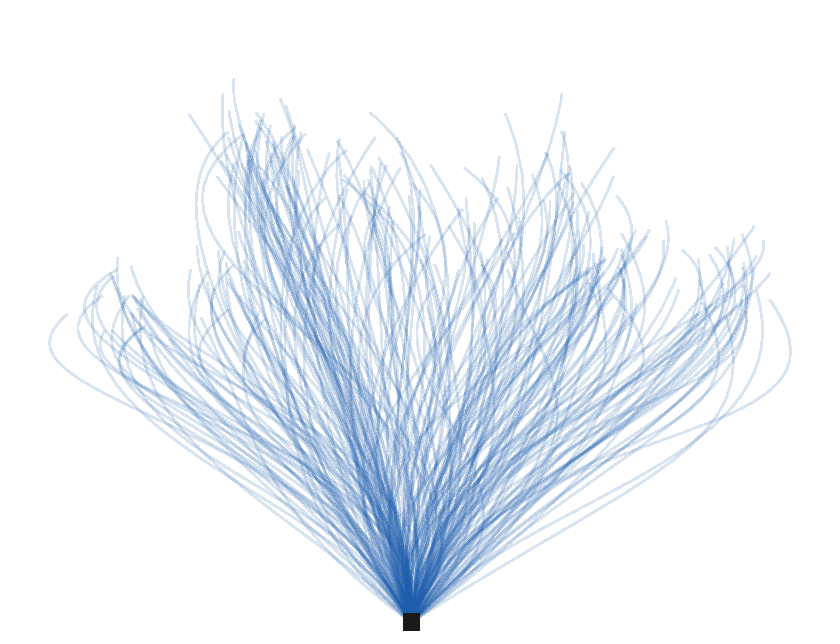
\includegraphics[width=5.6in]{fig/cover_art}};
  \fill[mach] ([xshift=0.62in]current page.north west) rectangle ([xshift=0.62in+2.4pt]current page.south west);
  \fill[rcpt] ([xshift=0.62in+7pt]current page.north west) rectangle ([xshift=0.62in+8.1pt]current page.south west);
  \fill[rcpt] ([xshift=0.62in+10.3pt]current page.north west) rectangle ([xshift=0.62in+11.4pt]current page.south west);
  \node[anchor=north west,inner sep=0pt,align=left,text=ink] at ([xshift=1.12in,yshift=-1.25in]current page.north west) {\fontsize{50}{54}\selectfont The Price\\[5pt]\fontsize{50}{54}\selectfont of Agency};
  \node[anchor=north west,inner sep=0pt,align=left,text=ink] at ([xshift=1.12in,yshift=-3.05in]current page.north west) {\fontsize{14}{20}\selectfont\itshape Freedom, measured. Theft, priced.\\\fontsize{14}{20}\selectfont\itshape No opinions required.};
  \node[anchor=south west,inner sep=0pt,align=left,text=ink] at ([xshift=1.12in,yshift=0.78in]current page.south west) {\sffamily\fontsize{12}{15}\selectfont Aaron Alai\\[2pt]\sffamily\fontsize{8.6}{12}\selectfont\color{muted}with Claude (Anthropic) as mathematical collaborator};
\end{tikzpicture}}
% ---------------------------------------------------------------- the index (its entries are written by design/make_index.py)
\newcommand{\indexopen}{\openpage\thispagestyle{plain}\renewcommand{\runninghead}{Index}\phantomsection\label{index}%
  \noindent\hspace*{-\ledgertotal}\parbox[t]{\dimexpr\textwidth+\ledgertotal}{\raggedright\fontsize{31}{35}\selectfont Index}\par\vspace{0.22in}%
  \noindent{\sffamily\fontsize{7.6}{10.4}\selectfont\color{muted}Words the book uses on nearly every page are listed at the passages that define them or turn on them. The theorems follow, by number.\par}\vspace{0.16in}%
  \begin{multicols}{2}\sffamily\fontsize{7.6}{10.6}\selectfont\raggedright\setlength{\parskip}{1.2pt}\setlength{\parindent}{0pt}}
\newcommand{\indexentry}[2]{\par\hangindent=1.1em\hangafter=1\noindent #1\enspace{\color{muted}#2}}
\newcommand{\indexclaims}{\par\vspace{1.0\baselineskip}\noindent{\bfseries Theorems and results, where stated}\par\vspace{0.3\baselineskip}}
\newcommand{\indexclose}{\end{multicols}}
% ---------------------------------------------------------------- key to the pages
\newcommand{\swatch}[1]{\tikz[baseline=-0.6ex]{#1}}
\newcommand{\keyrow}[3]{\noindent\makebox[0.42in][l]{#1}\parbox[t]{\dimexpr\linewidth-0.42in}{\raggedright\sffamily\fontsize{8.6}{12}\selectfont\textbf{#2}\hspace{0.6em}#3}\par\vspace{6pt}}
\newcommand{\pagekey}{\par\addvspace{0.9\baselineskip}\noindent\begin{minipage}{\linewidth}
 {\color{hair}\rule{\linewidth}{0.5pt}}\par\vspace{7pt}
 \keyrow{\swatch{\draw[hair,line width=0.5pt,fill=white] (0,-0.13) rectangle (0.26in,0.13);}}{No rule}{§1 and §2: the idea and the story. For every reader.}
 \keyrow{\swatch{\draw[mach,line width=1.7pt] (0.13in,-0.16) -- (0.13in,0.16);}}{Single blue rule}{§3 onward: theorems, mathematics, models. The machinery.}
 \keyrow{\swatch{\draw[rcpt,line width=0.8pt] (0.12in,-0.16) -- (0.12in,0.16);\draw[rcpt,line width=0.8pt] (0.12in+2.2pt,-0.16) -- (0.12in+2.2pt,0.16);}}{Double brass rule}{§6 and the public record: code, files, data. The receipts.}
 \keyrow{\swatch{\draw[fence,line width=1.3pt,dash pattern=on 4pt off 3pt] (0.13in,-0.16) -- (0.13in,0.16);}}{Dashed rule}{Chapter 12 only: a conjecture, fenced.}
 \vspace{-1pt}{\color{hair}\rule{\linewidth}{0.5pt}}\end{minipage}\par\addvspace{0.9\baselineskip}}
% ---------------------------------------------------------------- contents
\newcommand{\tocpart}[3]{\par\addvspace{13pt}\noindent\hspace*{-\ledgertotal}\makebox[\ledgertotal][l]{\sffamily\fontsize{8.4}{11}\selectfont\color{muted}Part #1}%
  {\sffamily\bfseries\fontsize{10}{13}\selectfont #2}\par\vspace{3pt}}
\newcommand{\tocchap}[3]{\noindent\makebox[1.7em][l]{\sffamily\fontsize{9}{15}\selectfont\color{muted}#1}{\fontsize{10.3}{15.5}\selectfont #2}%
  {\color{hair}\,\leaders\hbox to 0.5em{\hss.\hss}\hfill\,}{\sffamily\fontsize{9}{15}\selectfont\pageref{#3}}\par}
\newcommand{\tocessay}[2]{\noindent\makebox[1.7em][l]{}{\fontsize{10.3}{15.5}\selectfont\itshape #1}{\color{hair}\,\leaders\hbox to 0.5em{\hss.\hss}\hfill\,}{\sffamily\fontsize{9}{15}\selectfont\pageref{#2}}\par}
\newcommand{\tocfront}[2]{\noindent{\fontsize{10.3}{15.5}\selectfont #1}{\color{hair}\,\leaders\hbox to 0.5em{\hss.\hss}\hfill\,}{\sffamily\fontsize{9}{15}\selectfont\pageref{#2}}\par}
\newcommand{\frontsect}[2]{\openpage\thispagestyle{plain}\renewcommand{\runninghead}{#1}\phantomsection\label{#2}%
  \vspace*{0.35in}\noindent\parbox[t]{\linewidth}{\raggedright\fontsize{24}{28}\selectfont #1}\par\vspace{0.3in}}
% ---------------------------------------------------------------- displayed mathematics
\makeatletter
\newenvironment{dispmath}{\par\addvspace{9pt}\begingroup\centering$\displaystyle}{$\par\endgroup\addvspace{9pt}\@afterindentfalse\@afterheading}
\makeatother

\begin{document}
\pagenumbering{roman}
\begin{titlepage}\thispagestyle{empty}\vspace*{1.7in}
\noindent\hspace*{-\ledgertotal}\parbox[t]{\dimexpr\textwidth+\ledgertotal}{\raggedright
{\fontsize{44}{48}\selectfont The Price\\[4pt] of Agency}\par\vspace{0.42in}
{\fontsize{14}{20}\selectfont\itshape Freedom, measured. Theft, priced.\\No opinions required.}\par\vspace{2.6in}
{\sffamily\fontsize{11}{15}\selectfont Aaron Alai}\par\vspace{3pt}
{\sffamily\fontsize{9}{13}\selectfont\color{muted}with Claude (Anthropic) as mathematical collaborator}\par\vspace{0.5in}
{\sffamily\fontsize{8}{11}\selectfont\color{muted}Draft v0.50}}
\clearpage\thispagestyle{empty}\vspace*{\fill}
\noindent\parbox[b]{\textwidth}{\raggedright\sffamily\fontsize{7.8}{11.4}\selectfont\color{ink}
\textbf{The Price of Agency.} Draft v0.50, November 2026.\par\vspace{7pt}
Every script, results file and preregistration named in this book is in its repository:\\ \url{https://github.com/RandomInternetPreson/price-of-agency}\par\vspace{7pt}
To cite it: Aaron Alai, with Claude (Anthropic) as mathematical collaborator, \textit{The Price of Agency: Freedom, measured. Theft, priced. No opinions required.} Draft v0.50, 2026. \url{https://github.com/RandomInternetPreson/price-of-agency} \ doi:10.5281/zenodo.24599088\par\vspace{7pt}
\textcopyright\ 2026 Aaron Alai. The text and figures may be copied, translated and built on, for any purpose, with credit (Creative Commons Attribution 4.0 International). The code may be used for anything (MIT).\par\vspace{7pt}
The physics it stands on: arXiv:2608.00124 and arXiv:2608.18886.\par\vspace{7pt}
Set in TeX Gyre Pagella and Fira Sans, and built from the manuscript by the scripts in \texttt{design/}.}
\end{titlepage}
\pagenumbering{arabic}
\frontsect{Contents}{front-toc}
\tocfront{How to read this book}{front-howto}
\tocpart{I}{The Verdict and the Appeal}{partI}
\tocchap{1}{The sealed verdict}{ch1}
\tocchap{2}{The price of locality, in one chapter}{ch2}
\tocchap{3}{Apparent non-determinism: the claim, precisely}{ch3}
\tocpart{II}{One Agent: The Anatomy of Freedom}{partII}
\tocchap{4}{The Leaf and the Timetable}{ch4}
\tocchap{5}{The Gate}{ch5}
\tocchap{6}{The Frontier, and the Plateau}{ch6}
\tocchap{7}{Cheap Theft}{ch7}
\tocpart{III}{Watchers: Freedom Is Relative to an Observer}{partIII}
\tocchap{8}{The Watchers}{ch8}
\tocchap{9}{Habits and Coins}{ch9}
\tocpart{IV}{Towns: Freedom Is Social}{partIV}
\tocchap{10}{Neighbors}{ch10}
\tocchap{11}{The Fishing Town}{ch11}
\tocchap{12}{A Conjecture, Fenced}{ch12}
\tocpart{V}{The Ledger}{partV}
\tocessay{Why the self-anointed rule}{sec-why-the-self-anointed-rule}
\tocessay{The law’s own exhibit}{sec-the-law-s-own-exhibit}
\tocchap{13}{The Ledger}{ch13}
\tocchap{14}{What the Model Says to Do}{ch14}
\tocchap{15}{What Each Open Question Requires}{ch15}
\par\addvspace{13pt}\tocfront{Coda: The Whole Argument, Walked Once}{coda}
\par\addvspace{13pt}\tocfront{Appendices}{appx}
\par\addvspace{13pt}\tocfront{Index}{index}
\clearpage
\frontsect{How to read this book}{front-howto}

This book runs on two assumptions about the world, and only two:

\axioms{No one has perfect knowledge.}{Mistakes are inevitable.}

That is the entire list --- and because everything downstream leans on
these two sentences, they will return by name wherever a theorem
stands on one of them. If you accept those two sentences --- and no
physicist, economist, priest, or skeptic can demonstrate or prove otherwise --- then
everything that follows is either \emph{derived} from them or \emph{labeled} as
something less. (Every model in the book adds structure of its own ---
which signals exist, how errors correlate, what counts as survival ---
and each chapter's §5 prints that structure and says what travels
beyond it.) The labels are printed beside every claim:

\begin{itemize}
\tightlist
\item
  \istamp{PROVEN} --- a proof you can read, short enough to check by hand.
\item
  \istamp{EXACT} --- computed by exhaustive enumeration, no sampling, no
  approximation.
\item
  \istamp{NUMERICAL} / \istamp{MC} / \istamp{SIMULATION} --- computed with stated
  error, or by many simulated lifetimes with exact bookkeeping inside
  each; the weakest results in the book, and marked so.
\item
  \istamp{DATA} --- measured in the world by someone else and tabulated
  here; descriptive unless a design is named, and never a proof of a
  model.
\item
  \istamp{CONJECTURE} --- a potential pattern, not proven.
\item
  \istamp{SPECULATIVE} --- an interesting idea, fenced off so it cannot
  pretend to be a result.
\item
  \istamp{REFUTED — kept} --- something assumed a priori that the
  mathematics killed. There are several, and they are kept, because
  you may have had the same assumptions.
\end{itemize}

Every chapter is built the same way: §1--2 are for every reader; §3
onward for those who want the machinery; §6 for anyone who trusts
nothing --- the best kind of reader this book can have.

\pagekey

And the book has two doors. Part I is the physics: the license under
everything after it, in three short chapters. A reader who came for
the schedule and not the particle can start at the harbor in Chapter 4
and miss nothing the measuring depends on; Chapter 3 says in one
sentence what the physics contributes, and Part I is there whenever
the license is questioned.

One more rule. The word \emph{theft} appears throughout. It is defined
mathematically in Chapter 7 --- a measurable displacement, like a dent
measured with calipers --- before it is ever used as an accusation. If you
dislike the word, strike it and read the equations. They do not change.

\renewcommand{\partlist}{\partline{1}{The sealed verdict}{ch1}\partline{2}{The price of locality, in one chapter}{ch2}\partline{3}{Apparent non-determinism: the claim, precisely}{ch3}}\partopen{I}{The Verdict and the Appeal}{partI}\renewcommand{\runninghead}{The Verdict and the Appeal}

\chapteropen{Part I. The Verdict and the Appeal}{1}{The sealed verdict}{ch1}

There is a sentence that has been said to students, to prisoners, to
employees, to whole populations, for about a century, always with the
same borrowed confidence:

\saying{``Free will is an illusion.''}

Notice what kind of sentence that is. It is not an argument --- arguments
can be answered. It is a claim of \emph{authority}: somewhere, allegedly, in
mathematics you have not read, the question was closed, and your
protest is not a position but a symptom. You are, the sentence implies,
a very complicated rock --- and everything that follows from being a rock
follows quietly: a rock cannot be robbed of choices it never had; a rock
cannot be owed an education it could not use; what is done \emph{to} a rock
is arranged, not inflicted.

Living under an unanswerable sentence is a particular kind of
confinement. This book calls it the sealed verdict: a judgment passed
on your deepest nature, in a court you are forbidden to enter,
delivered to you as final. Most people respond to a sealed verdict in
one of two ways. They ignore it, and live as if free, with a small
unpaid debt of doubt. Or they accept it, and discover
that acceptance is oddly convenient for whoever is speaking.

There is a second sentence, politer, usually from kinder mouths, that
does the same work by shrug instead of decree:

\saying{``It doesn't matter whether you have free will or not.''}

Notice what this one accomplishes. It concedes nothing and closes
everything: no need to read the mathematics, because nothing allegedly
hinges on it --- live your life either way. The full answer to the
second sentence is this entire book. The short answer: it matters, and
it matters in the way things matter that can be counted. Whether a person's actions are partly
their own decides whether they can be \emph{robbed} --- whether taking their
time, their options, their room to be wrong is an injury or merely a
rearrangement of objects; whether an education is owed to something
that could use one; whether what lands on a life was inflicted or just
occurred. Every one of those questions turns out, in the chapters
ahead, to be a measurable quantity with a price. And the shrug has
been the accounting instrument by which that price is set to zero.
``It doesn't matter'' is what it sounds like when the bill is being
sent to someone else.

This book does not argue that you have free will. The wording is
exact: \emph{it does not claim to prove freedom exists.} No honest person currently can. What can
be done --- what has now been done, with theorems --- is smaller and
sharper: the \emph{authority} of the sentence can be revoked. It can be shown,
exactly, what physics does and does not require; it can be shown that
the deterministic reading is a choice with a price sheet, not a
conclusion with a proof; and it can be shown that the verdict
was never entered --- that at every size at which the question has been
priced, the universe declines to sign it.

Revoking an authority is not a metaphorical act. It requires arithmetic
the authority cannot survive. Chapter 2 is that arithmetic.

And then --- because a door is only interesting if something lies beyond
it --- the rest of the book walks through. If a universe \emph{permits} what this
book calls apparent non-determinism, then agency becomes a quantity: a
thing with an anatomy, a price list, thresholds, floors, and thieves.
The remaining chapters measure it.

\chapteropen{Part I. The Verdict and the Appeal}{2}{The price of locality, in one chapter}{ch2}

In 1964, John Bell proved that three innocent-sounding assumptions
cannot all survive contact with experiment. Stated plainly:

\begin{enumerate}
\def\labelenumi{\arabic{enumi}.}
\tightlist
\item
  \textbf{Locality.} Influence does not travel faster than light.
\item
  \textbf{Determinism.} Outcomes are fixed by prior facts.
\item
  \textbf{Measurement independence.} The experimenter's choice of what to
  measure is statistically independent of the hidden facts of the thing
  measured --- in slogan form: \emph{the universe does not rig your questions
  to fit its answers.}
\end{enumerate}

Experiments violate Bell's inequalities. Therefore at least one
assumption is false. Physicists mostly shop between abandoning the
first (resulting in spooky action) and abandoning single outcomes altogether (resulting in many
worlds). The third exit --- that measurement independence fails, not by
cosmic conspiracy but lawfully and partially --- was long treated as the
disreputable door. Then in 2010, Michael Hall asked the question that
changes the register of the whole debate: \emph{if you take the third exit,
what is the fare?} And he answered it exactly, for the simplest case:
to reproduce the quantum correlations of two entangled particles with a
local, deterministic model, measurement independence must be relaxed by
precisely \((\sqrt{2}-1)/3\) --- about 13.81\%. Not all of it. Not none of it.
That number.

A door with a posted price is a different object from a forbidden door.

\booktikzfloat{fig/exits.tex}{2.1}{The three exits from Bell's theorem. The first two are where physicists mostly shop. The third was long treated as the disreputable door, and it is the one with a fare posted. The picture ranks nothing.}

Hall priced the two-particle case and one fragment of the three-particle
case, and left the general problem open in 2011. It stayed open for
fifteen years. The solution --- the mathematics this book's lineage rests
on --- computes the exact minimum relaxation for the full faithful
statistics of the canonical multiparticle experiments, certified in
exact arithmetic out to twenty-two particles, and finds the answers are
not a mess but a law --- stated there for every size, and since proven
for every size {[}\tagword{PROVEN} / \tagword{EXACT}; the published record --- arXiv:2608.00124,
Zenodo DOI 10.5281/zenodo.21445609{]}:

\begin{dispmath}F = \frac{R}{2(R+1)}, \qquad \text{where } R \text{ doubles with every second particle.}\end{dispmath}

\noindent One third at three particles. Two fifths at five. Four ninths at seven.
8/17, 16/33, 32/65 --- a staircase, climbing with perfect regularity
toward, and this is the theorem that matters most, a \textbf{ceiling it can
never reach: \(F \le 1/2\), at every size, forever.} The universe's
statistics never require measurement independence to be relaxed by more
than half. Total determinism-by-conspiracy is never \emph{forced}. The
door is never welded.

\bookfigurefloat{fig/staircase.pdf}{2.2}{The fare for the third exit, by the number of particles in the experiment: the share of measurement independence a local, deterministic account must relax. It rises with every second particle and never reaches one half. From the published record (arXiv:2608.00124), certified through twenty-two particles.}

\begin{ruled}

\rulednote{\textbf{The machinery}\\for those who want it}The staircase was the first paper. There is now a second {[}\tagword{CONJECTURED}
\tagword{SURFACE}, certified exactly at the quantum point and at six rational
points; the published record --- arXiv:2608.18886{]}, and Part V takes
its exhibit from it. The original experiment that
started all of this --- two particles, two detectors --- turns out to have
not one posted price but two, on two different doors: how much
measurement independence a local account must relax, and how
efficient its detectors are permitted to be. The second paper computes
the exact exchange rate between the two --- relax less of one, pay
more of the other, at a rate written down in closed form --- exact to the digit where it has been certified, conjectured between --- and then
does something no result in this lineage had done before: it finds a
specific, physical quantity that the standard experiment is
mathematically incapable of seeing --- checked only at the percent level
through four decades of the most scrutinized experiments in physics,
never below it, which is where the surviving accounts live --- and it
hands over a protocol that any well-equipped laboratory can run to
measure it there. Whichever way that measurement comes out, a named
family of accounts is bounded an order of magnitude tighter than the
record now holds it. And one thing it cannot do, whichever way it
comes out: touch the license. The ceiling above was proven by
arithmetic over every strategy a local account could adopt; no
coincidence count can raise it or lower it. The scan audits which
ledger the surviving accounts pay in --- never whether the door is
open. (And to keep this book's own fence intact: that exchange rate
prices trade-offs \emph{within} the surviving local accounts, between their
two internal ledgers --- never \emph{across} the exits from Bell's theorem,
which remain unranked.) An exact price, an unmeasured column, an
instrument anyone can pick up: the second half of this book uses all
three.

\end{ruled}

Now, exactly what this result licenses and what it does not:

\textbf{It does not prove you are free.} A fully superdeterministic universe
remains logically consistent. So does ordinary quantum mechanics with no
hidden layer at all. The staircase takes no side.

\begin{ruled}

\rulednote{\textbf{The machinery}\\for those who want it}One argument, made by the author of the two papers and labeled as an
argument, not a result. To compare exits at all, a common currency must
be chosen --- and here is a principled candidate: score each exit's extrapolation against the
constraints every \emph{other} science already answers to. Thermodynamics.
Information theory. No privileged observer standing outside the
universe. No effects preceding causes. Every other discipline must
tell its story through that highly constrained lens; the exits from
Bell's theorem have historically enjoyed a free pass from it --- perhaps
precisely because this third exit went unpriced. Under that currency,
the priced exit is the conservative one: no influence outrunning
light, no unobservable proliferating worlds, no retrocausality --- full
congruence with the physics everything else already obeys. Under
other currencies --- dynamical parsimony, or the refusal of hidden
variables altogether --- other exits win, which is why physicists still
disagree, and why this paragraph is an argument. There is a second
candidate currency, worth naming with its own caveat attached: the
capacity to be audited. The canonical forms of the other exits are
built to agree with quantum mechanics everywhere, which makes them
untestable against it by design --- their falsifiable cousins exist,
but purchase their testability by disagreeing with the record in
territory already measured, where the record squeezes them. The exit
priced in this book turned out to carry its testable content in a
column no experiment had measured --- congruent with everything ever
recorded, and still auditable {[}the sequel, arXiv:2608.18886; the
exhibit that closes Part V tells that story --- the unmeasured quantity,
the theorem that hid it, the protocol that measures it{]}. And it does more than survive there. The paper that priced the exit also built it --- an explicit local mechanism, with no stochastic ingredient, that pays exactly the posted price --- and both the price and the mechanism come with things an experiment can look for. The solved detection sector predicts a fringe in the total coincidence rate as the analyzers turn (the exhibit of Part V), in a quantity recorded for forty years at the percent level and never below it. And the mechanism itself leaves a fingerprint on the correlation curve every Bell experiment measures: a softening of its extremes --- where the quantum curve reaches perfect agreement and perfect disagreement, the mechanism falls short by up to about a percent, concentrated between the Bell angles. Resolving the mechanism more finely shrinks that softening and moves it between the angles tested; at every resolution tried it keeps the same shape, and whether it survives to the continuum is a question the paper leaves open and says so. No other account on the record is all of these at once: local, deterministic, priced below total conspiracy at every size, built as an explicit mechanism, and specific about what an experiment should find --- a softening in a curve every Bell experiment already records, and a fringe in a sum that quantum mechanics says is flat. And whichever way those experiments come out, the ceiling of this chapter stands: the scan decides which ledger the surviving accounts pay in, never whether the door is open. Under that currency too, the priced
exit stands alone --- and the same caveat applies: an argument, not a
theorem. But the reader is entitled to notice which currencies the
rest of science is already paying in.

\end{ruled}

\textbf{It proves that no one can claim mathematics took the side against
you.} Anyone asserting that physics \emph{requires} the fully rigged
universe is now making a claim with an exact counter-theorem. The
sealed verdict --- its authority borrowed from proofs that turn out not
to lend it --- is vacated on appeal. What remains is, \emph{just, like, your opinion, man} --- and you are free
to decline opinions.

Hold on to the shape of what just happened, because the entire book
repeats it at larger scales. A question that sounded metaphysical
(\emph{am I free?}) was converted into a question with units (\emph{what is the
minimum price of pretending otherwise?}), and the answer came back
bounded, exact, and universal. Freedom was not proven. Freedom was
\emph{priced} --- and its price, in measurement independence, was capped at
one half.

The next chapter names the thing on the far side of the door --- apparent
non-determinism --- and states exactly
what the physics contributes to it (a license, never a number) before
the measuring begins.

\chapteropen{Part I. The Verdict and the Appeal}{3}{Apparent non-determinism: the claim, precisely}{ch3}

Every framework has one chapter where a careless sentence would poison
all the others. This is that chapter, so it will be short and it will be
exact.

The thing on the far side of the door needs a name that does not smuggle
in a conclusion. \emph{Free will} is a courtroom of a phrase --- two thousand
years of theology and neuroscience shouting in it. This book uses a cooler term:
\textbf{apparent non-determinism}, AND for short, and in mathematics the
symbol \(\delta_A\). Here is what it means, in one breath: \emph{an entity exhibits
AND to the degree that its actions cannot be predicted from its local
circumstances.} A rock exhibits none --- give the slope and the rain,
and the rock is given. A person may exhibit a great deal --- or,
under certain conditions this book will price with uncomfortable
precision, almost none.

Note what the definition does not mention: souls, quantum mechanics,
consciousness, or the truth about determinism. AND is \emph{apparent} ---
defined relative to what an observer can predict --- which is exactly what
makes it measurable, and measurability is the entire premise.

Now the sentence that must be said with total clarity, because every
hostile reader arrives with its refutation pre-loaded, aimed at a claim
this book does not make:

\textbf{The physics of Chapter 2 contributes a license, never a number.}

The staircase does not cause your Tuesday. The ceiling \(F \le 1/2\) does not
govern wages, and 8/17 at nine particles implies nothing about nine
senators. Anyone who tells you this book derives economics from quantum
mechanics has not read this paragraph, and you may return them to it.
What the physics contributes is one thing, and it is not small: it
guarantees the \emph{possibility class is open}. Before Chapter 2, ``agents
whose actions are partly independent of circumstance'' was a hypothesis a
determinist could dismiss with borrowed authority. After Chapter 2, it
is a standing possibility of the universe, priced and bounded, that no
one can strike from the table. Everything measured in the rest of this
book lives on that table --- and lives or dies by its own evidence, in its
own units, exactly as the survival of chemistry does not depend on
re-proving atoms in every reaction.

One question remains before the measuring starts: why did settling the
physics matter, if the numbers never transfer? Because of what the
alternative licenses. If agents were rocks \emph{to every possible observer}
--- if the universe published a complete state from which every action
followed --- then nothing could be stolen from them, and the theft this
book prices would be a category error, like robbing gravity. The
license says no such publication is forced. The ledger itself is
narrower than the license and survives either way: it is defined in a
seat, from what an observer with incomplete information can predict
(Part III), and a deterministic agent with private knowledge scores on
it exactly as a stochastic one does. What the license removes is the
dismissal --- that the whole ledger is about nothing. It converts every
coercion from a neutral arrangement of matter into a \emph{possible taking},
and possible takings can be measured, audited, and charged for. That conversion is the door. The
rest of the book walks through it.

\renewcommand{\partlist}{\partline{4}{The Leaf and the Timetable}{ch4}\partline{5}{The Gate}{ch5}\partline{6}{The Frontier, and the Plateau}{ch6}\partline{7}{Cheap Theft}{ch7}}\partopen{II}{One Agent: The Anatomy of Freedom}{partII}\renewcommand{\runninghead}{One Agent: The Anatomy of Freedom}

\chapteropen{Part II. One Agent: The Anatomy of Freedom}{4}{The Leaf and the Timetable}{ch4}

\routemap{\mapcellbox{0}{§\,1}{The idea}{ch4-s1}\mapcellbox{0}{§\,2}{The story}{ch4-s2}\mapcellbox{1}{§\,3}{The theorems}{ch4-s3}\mapcellbox{1}{§\,4}{The mathematics}{ch4-s4}\mapcellbox{1}{§\,5}{The model}{ch4-s5}\mapcellbox{2}{§\,6}{The code}{ch4-s6}}

\sect{§\,1}{The idea, in plain words}{ch4-s1}

The two axioms say what this book assumes. One further decision, made in
this chapter, says how it measures --- and everything measured afterward
stands on it: \textbf{freedom needs two rulers, not one.}

The obvious single ruler --- call it unpredictability --- asks: after seeing
someone's circumstances, how much doubt remains about what they will do?
It sounds right. It is measurable. And it fails, in a way so instructive
that the failure became the foundation. Because two very different
things score high on unpredictability: a person steering their own life,
and a dropped leaf tumbling in the wind. And two very different things
score low: a coerced person, and a competent one in a world where the
right move is obvious.

So this chapter splits the measurement in two. The first ruler,
\emph{independence}, keeps the old question: how little do circumstances
predict your actions? The second, \emph{aim}, asks the question the leaf
fails: how much do your actions have to do with what actually comes
next? Freedom, as this book will use the word from here on, means scoring
on both rulers at once --- and the entire book is a map of what that
double score costs, who pays it, and who takes it.

\sect{§\,2}{The story: the harbor}{ch4-s2}

Stand on a harbor wall in a stiff wind and watch three people.

The \textbf{ferry captain} runs the posted schedule. Weather within limits,
she sails at the top of the hour to the island and back, the same
crossing she has made four thousand times. And note something easily
missed: she is never \emph{wrong}. Her seamanship is real and her crossings
are flawless. But anyone holding the timetable and a weather report can
predict her whole day without watching her once. Her poverty is not
error. It is that everything she does was already written in her
circumstances.

The \textbf{lost tourist} is her opposite. He has no destination, no map he
trusts, and he wanders the quays turning wherever the crowd or a smell
or a seagull suggests. Nobody can predict his next turn --- not you, and
not really him. By the single ruler, he is the freest person on the
harbor. And he is going nowhere. His unpredictability is genuine, and
it serves nothing.

Then the \textbf{sailor} casts off --- heading upwind. Watch him closely,
because his behavior is strange by both of the other standards. He does
not do what the wind says: he tacks, cutting angles the gusts never
dictated, sometimes turning \emph{toward} rough water. An observer reading
only the wind and the harbor cannot call his moves. But neither is he
wandering: every strange angle serves the same unwavering destination,
and he arrives. The wind pushed everyone on that water today; the
captain's route was written by it and the timetable, the tourist
scattered on it, and the sailor \emph{used} it --- visible in his wake as the
only track that disagreed with the wind and still ended at the chosen
port.

\booktikzfloat{fig/harbor.tex}{4.1}{One harbor, one wind, three tracks.}

Independence without aim is the tourist. Aim without independence is
the captain. The sailor is what the two rulers, together, are built to
find.

\begin{machinery}{\textbf{The machinery}\\for those who want it\\[3pt]{\color{muted}Story resumes:\\page~\pageref{ch5}}}

\sect{§\,3}{The theorems}{ch4-s3}

Three results fence the space the two rulers draw. Stated here in words;
formally in §4; proofs in the theorem file.

\claimhead{Theorem 1}{The sage ceiling — Axiom 1, made quantitative}{PROVEN}{1}

\label{claim-0}

\noindent \emph{Even a perfect agent ---
complete knowledge of its own future, unlimited deliberation --- cannot
reach total independence. Its remaining predictability equals exactly
what its environment already knew about that future.} You can never
rationally be less predictable than your world is informative; ignoring
a genuinely telling circumstance is not freedom but error. Every
environment posts a ceiling, and the ceiling belongs to the environment. Cybernetics reached a neighboring sentence fifty years earlier --- Conant and Ashby's good-regulator theorem (1970), that every competent regulator must carry a model of what it regulates --- and Theorem 1 is in its spirit: the sage's predictability is the model it cannot help carrying. The difference is the quantity measured. Conant and Ashby bound the regulator's structure; Theorem 1 prices its independence.

\claimhead{Theorem 2}{Complementarity}{PROVEN}{1}

\label{claim-1}

\noindent \emph{The environment's information
about the future is a fixed pot, split exactly two ways: it is
simultaneously the ceiling on the captain's aim and the floor under
the sailor's predictability.} One quantity, two debts. (The partition above is a statement about information
specifically; if aim is scored by raw success rate instead, the two
quantities no longer sum to one --- the audit is printed in §5.)

\claimhead{Proposition 3}{Starved is not free}{PROVEN}{1}

\label{claim-2}

\noindent \emph{Strip an agent of
deliberation and its unpredictability rises --- toward the leaf.} On the
single ruler, the most deprived agent scores as the most free. This
inversion is why the single ruler is not merely imprecise but dangerous,
and Chapter 7 will show it is exploitable.

\sect{§\,4}{The mathematics}{ch4-s4}

The two rulers, built from plain parts.

\emph{Doubt is counted in bits.} One bit is one fair coin-flip of remaining
uncertainty; three bits, three coin-flips. The standard name for
counted doubt is \emph{entropy}, written \(H\).

\textbf{Ruler one --- independence.} Let \(A\) be the action taken and \(E\) the circumstances an observer sees. \(H(A \mid E)\) counts the observer's remaining doubt about \(A\) \emph{after} seeing \(E\). Scale it by the doubt a total stranger
would have (\(\log_2\) of the number of possible actions) and it lands on a
0-to-1 dial:

\begin{dispmath}\delta_A = \frac{H(A \mid E)}{\log_2 |A|}\end{dispmath}

\noindent \(\delta_A = 0\): the captain --- circumstances leave no doubt. \(\delta_A = 1\): the tourist --- circumstances say nothing.

\textbf{Ruler two --- aim.} Let \(F\) be the future the agent is steering toward ---
a state of the world the action is a bet on (where the fish are, what
the weather does, what the market will come to want), never an outcome
the action itself produces. \(F\) is exogenous to \(A\) everywhere in this
book; what that rules out, and why the audit of Chapter 13 needs it, is
said there. One more thing aim is not: a success rate. Information is
blind to relabeling --- an agent who always does the opposite of what the
future calls for tracks it perfectly and fails every time --- so aim
measures the capacity to track the future, not whether the tracking
was used well. The theorems of this book are about that capacity; a
success score adds a decoding the rulers do not see. For the agents of
this book the two move together, because every agent here is built to
seek reward and so decodes in its own favor --- the perverse case is an
agent who knows the future and chooses to lose. Where the book prices a
loss of aim as a loss, that is the agent it has in mind.
The information the action carries about that future --- written \(I(A;F)\), the number of bits of doubt about \(F\) that watching \(A\) removes --- measures
whether behavior is \emph{about} anything. Scaled the same way:

\begin{dispmath}\text{aim} = \frac{I(A;F)}{H(F)}\end{dispmath}

\noindent The tourist: \(\delta_A = 1\), aim \(= 0\). The captain in fair weather: \(\delta_A = 0\), aim \(= 1\). The sailor lives where both are high --- and Theorems 1 and 2
say exactly how high both can simultaneously be.

\booktikz{fig/plane.tex}{4.2}{Where the three stand on the two rulers. The single ruler of unpredictability reads only the vertical scale, on which the tourist outranks everyone. How far up and to the right anyone can go is Chapter 6.}

\textbf{Theorem 1, formally.} For an agent with full knowledge of \(F\) and ample deliberation, the acted policy is \(A = F\), so \(H(A \mid E) = H(F \mid E)\), and

\begin{dispmath}\delta_A(\text{sage}) = \frac{H(F \mid E)}{\log_2 |A|}\,.\end{dispmath}

\noindent The sage's ceiling is the environment's ignorance of the future --- one
line, once the definitions exist. \textbf{Theorem 2} follows by splitting
\(H(F) = H(F \mid E) \allowbreak + I(F;E)\): the second term is what the vane can capture
(its aim ceiling) and the first is what the sage cannot shed (its
predictability floor). The two debts sum to the whole pot.

\sect{§\,5}{The model, and its audits}{ch4-s5}

The world: a future \(F\) with \(n\) equally likely possibilities; an environment signal that reveals \(F\) with probability \(1-s\); a knowledge signal that reveals \(F\) with probability \(e\); an agent acting on the exact
Bayesian posterior, with deliberation controlled explicitly. All
quantities computed by exact enumeration --- no simulation, no fitted
parameters. (The agent is the standard bounded-rational one --- a Bayesian posterior sharpened by a single deliberation parameter, the form Ortega and Braun derived from information-processing costs in 2013 --- so nothing in the engine's driver is this book's invention. What the book adds is the second ruler held up to a driver already standard in its field.)

Audits, as the opening pages promised. Theorem 1 was machine-checked on five
hundred randomized worlds --- arbitrary priors, arbitrary asymmetric
channels --- with worst-case error at the limit of computer arithmetic.
Theorem 2 was checked the same way (no violations; equality exactly
where the proof says) and additionally stress-tested at alphabet sizes
up to 64. The complementarity identity is information-specific: re-run
with raw success rate in place of \(I(A;F)\), the two quantities no longer
sum to one, and no result in this book leans on the version that fails.
Proposition 3 is an exact limit of the model class and was replicated
under a second, independent model of deliberation in Chapter 7's
machinery --- where the \emph{direction} of the starved agent's drift turns out
to depend on what a mind falls back on when thought is taken, a fork
with consequences of its own.

\end{machinery}

\begin{receipts}{\textbf{The receipts}\\for anyone who\\trusts nothing}

\sect{§\,6}{The code}{ch4-s6}

\begin{itemize}
\tightlist
\item
  \texttt{code/\allowbreak{}delta\_\allowbreak{}A\_\allowbreak{}v1.\allowbreak{}py} --- both rulers computed across the full
  (education × noise) landscape; the four corner characters of this
  chapter appear as exact values.
\item
  \texttt{code/\allowbreak{}verify\_\allowbreak{}theorems.\allowbreak{}py} --- the five-hundred-world checks of
  Theorems 1 and 2.
\item
  \texttt{code/\allowbreak{}dichotomy\_\allowbreak{}scaling\_\allowbreak{}and\_\allowbreak{}audits.\allowbreak{}py} --- Theorem 2 at alphabet sizes
  16--64 on randomized channels; the success-rate audit.
\item
  Formal statements and proofs: \texttt{docs/\allowbreak{}THEOREMS\_\allowbreak{}v1.\allowbreak{}md}.
\end{itemize}

\end{receipts}

\chapteropen{Part II. One Agent: The Anatomy of Freedom}{5}{The Gate}{ch5}

\routemap{\mapcellbox{0}{§\,1}{The idea}{ch5-s1}\mapcellbox{0}{§\,2}{The story}{ch5-s2}\mapcellbox{1}{§\,3}{The theorem}{ch5-s3}\mapcellbox{1}{§\,4}{The mathematics}{ch5-s4}\mapcellbox{1}{§\,5}{The model}{ch5-s5}\mapcellbox{2}{§\,6}{The code}{ch5-s6}}

\sect{§\,1}{The idea, in plain words}{ch5-s1}

Here is the finding of this chapter in one sentence: \textbf{learning buys you
no independence at all --- none --- until what you know beats what your
surroundings already tell you; and the moment it does, independence
arrives all at once.}

The natural assumption --- the one most readers will bring, because it
was brought here first too --- is the opposite: the comfortable belief that every bit of education makes a person a bit
freer, smoothly, like filling a glass. The mathematics refused it. What it
handed back instead was a threshold: a gate. Below the gate, education
changes what you know but not what you do, because acting on weak
knowledge against a clear world is simply a mistake, and rational people
don't make it. Above the gate, your own knowledge outranks the world,
and your behavior stops being readable from your circumstances.

Education here means more than school. It is whatever leaves a person
knowing something their surroundings do not announce: a class, a
trade, an hour alone with a problem, years among the people they live
with. The gate does not ask where the knowledge came from. It asks how
often it is right.

One consequence deserves its own paragraph, because it runs against
instinct. \emph{The clearer and more stable a person's world, the higher
their gate.} Someone whose environment is orderly, legible, fully
administered --- where the ``right'' move is always obvious from the
situation --- needs \emph{more} education before any of it purchases
independence, not less. Order is not neutral. Order raises the bar.

\sect{§\,2}{The story: the intersection}{ch5-s2}

Imagine learning to drive in a city where every intersection has a
working traffic light. You are given driving lessons --- theory, judgment,
the physics of wet roads. Are you freer for it? Watch your actual
behavior: at every light you do what the light says, exactly like every
driver who never took your lessons. Your knowledge is real, but the
world is so legible that following it is always the right call. Anyone
watching the lights can predict you perfectly. Your lessons bought you
nothing visible --- yet.

\booktikzfloat{fig/intersection.tex}{5.1}{The same drivers and the same lessons. Only what the intersection tells them has changed.}

Now the storm knocks the lights out. Suddenly the intersection says
nothing, and the drivers split: most freeze or follow the car in front ---
still readable, now from each other. But the driver whose training
finally \emph{exceeds} what the intersection offers makes her own call ---
yield here, roll there --- and for the first time, watching the
intersection tells you nothing about her. Same driver, same lessons.
The lessons crossed the gate only when the world stopped answering
first. That is the whole theorem, lived: education pays nothing until
it wins the argument with your surroundings --- and a world of perfect
traffic lights is a world where almost no one's education ever wins.

One more turn at the same intersection. The lights are out and her
training is good --- but the two kinds of mistake are not priced alike.
If she follows the car in front and it goes badly, she has a dented
bumper and company. If she makes her own call and it goes badly, she
loses the car, and with it the job the car gets her to. At those
prices she follows the car in front, and she is right to. What decides
it is not what she knows. It is what one mistake of her own would cost
her, set against a mistake made in company: her \textbf{mistake budget}.
The theorem below gives the number. In a world that is right half the
time, lessons open the gate once they are right more than fifty times
in a hundred. Let her own mistake cost ten times the shared one, and
the same lessons must be right ninety-five times in a hundred before
she acts on them. Her lessons did not get worse. The price of using
them went up.

\begin{machinery}{\textbf{The machinery}\\for those who want it\\[3pt]{\color{muted}Story resumes:\\page~\pageref{ch6}}}

\sect{§\,3}{The theorem}{ch5-s3}

\claimhead{Theorem 5}{Activation threshold}{}{0}

\label{claim-3}

\noindent \emph{In the model of §5, with environment reliability \(1-s\) and education fidelity \(e\), a rational agent's independence \(\delta_A\) is exactly zero whenever \(e < 1-s\), and strictly positive whenever \(e > 1-s\). The gate sits at}

\begin{dispmath}e^{\ast} = 1 - s\end{dispmath}

\noindent \emph{and its location does not depend on how finely the future is divided
(proven and verified for every alphabet size tested, 4 through 64).}
\istamp{PROVEN}

\bookfigure{fig/gate.pdf}{5.2}{Independence against education in two worlds, computed exactly in the model of §5 with sixteen possible futures. Below the gate nothing is bought; at the gate independence arrives at once. The orderly world sets its gate twice as high.}

Below the gate, the agent's behavior has a name in economics: an informational cascade (Banerjee 1992; Bikhchandani, Hirshleifer and Welch 1992) --- the rational discarding of a private signal when the public one is more reliable. Cascade theory studies the sequence of such decisions and how fragile it is. Theorem 5 is in its spirit and asks a different question: where the threshold sits, as a race between two reliabilities --- and finds the answer indifferent to how finely the future is divided.

In words: education fidelity plus environmental noise must exceed one.
Your knowledge and your world are in a reliability race, and only the
winner steers you.

\claimhead{Theorem 5b}{The mistake-budget gate}{EXACT}{1}

\label{claim-4}

\noindent \emph{The gate above
assumed a mistake costs the same whichever way you make it. Let a self-directed mistake cost \(\kappa\) times a conformist one --- the arithmetic
of living without a buffer, where one wrong bet of your own means
eviction --- and the gate moves to}

\begin{dispmath}\frac{e^{\ast}(\kappa)}{1 - e^{\ast}(\kappa)} \;=\; \frac{\kappa(1-s)}{s} + (\kappa - 1)\Bigl(1 - \frac{1}{n}\Bigr),\end{dispmath}

\noindent \emph{recovering \(e^{\ast} = 1-s\) exactly at \(\kappa = 1\) and rising with \(\kappa\).} The second
term is the case where both sources are wrong --- paid once by the
conformist, \(\kappa\) times by the self-directed --- and it keeps the number of
options in the formula: more ways to be wrong, a higher gate. At \(\kappa = 10\) in a half-noisy world, the gate sits at 0.936
with two options, 0.947 with eight, and under 0.95 with any number:
near-perfect knowledge required before independence is rational. The consequence deserves
plain statement: \textbf{a person can stand well above the education gate
and remain rationally conformist --- for want of a mistake budget.}
Environments that permit mistakes are not a kindness; they are a
precondition. And a mistake budget, like time, is a resource that can
be taken: a zero-buffer life is a welded gate wearing different
clothes. The gate assumes
the agent knows its own reliability. With noisy self-knowledge, the
mistake ratio that maximizes a population's \emph{per-decision accuracy} is
one where the population sits at its gate; below one where most sit
above it (a margin silences people who should act); and without bound
where most sit below it and do not know it --- there, the
accuracy-optimal rule is that nobody acts on their own judgment. That
last case is the shared-tutor town of Chapter 11: the most accurate
town per decision, and the one that starves. Accuracy and survival
part company exactly there, which is why Chapter 14's first rule ---
past the gate --- comes before its others, and why the \(\kappa\) a zero-buffer
life actually imposes, around ten, is justified by neither objective.
(Who gets to buy mistake budgets back, and at whose expense,
is Chapter 13's business. Organizations have long had words near this one --- \emph{slack}, in Cyert and March's behavioral theory of the firm (1963); \emph{psychological safety}, in Edmondson's study of teams (1999) --- and the mistake budget is in their spirit while being a sharper object: a ratio, \(\kappa\), that moves a proven gate by a computable amount.)

\sect{§\,4}{The mathematics}{ch5-s4}

Two quantities, built from plain parts.

\emph{Independence}, \(\delta_A\), asks: after seeing your circumstances, how
uncertain does an observer remain about your action? Uncertainty is
measured in bits --- one bit is one fair coin-flip of doubt. If your
circumstances pin your action completely, the observer holds zero bits
of doubt: \(\delta_A = 0\), the rock. If circumstances say nothing about your
action, doubt is maximal: \(\delta_A = 1\). (Formally: \(\delta_A = H(A \mid E)/\log_2 |A|\), the conditional entropy of action given environment, scaled to \([0,1]\).)

\emph{The gate}, derived. Your environment \(E\) points at your future correctly with probability \((1-s) + s/n\) --- right most of the time, uniformly
confused otherwise. Your education \(K\) points correctly with probability \(e + (1-e)/n\). When the two disagree, a rational agent asks: which source
is more likely to be right, given exactly this disagreement? Bayes'
rule makes it a ratio of the two channels' odds:

\begin{dispmath}\begin{aligned}\text{follow } K \;&\Longleftrightarrow\; \frac{e + (1-e)/n}{(1-e)/n} \;>\; \frac{(1-s) + s/n}{s/n}\\[4pt]&\Longleftrightarrow\; \frac{n\,e}{1-e} \;>\; \frac{n\,(1-s)}{s}\\[4pt]&\Longleftrightarrow\; e\,s > (1-s)(1-e)\\[4pt]&\Longleftrightarrow\; e + s > 1.\end{aligned}\end{dispmath}

\noindent Four lines. Notice the alphabet size \(n\) cancels --- the gate does not care
how complicated the future is, only who is more reliable about it.
Below the gate the agent follows \(E\) everywhere (\(\delta_A = 0\) identically);
above it, the agent defects to its own knowledge wherever the two
disagree, and \(\delta_A\) jumps.

\emph{The mistake-budget gate}, derived the same way. On a disagreement the
posterior's weights on the environment's future, on knowledge's, and
on neither stand in the
proportion \(1 + n(1-s)/s\) to \(1 + n\,e/(1-e)\) to \(n - 2\). Acting with the
environment costs 1 when it is wrong; acting on knowledge, \(\kappa\):

\begin{dispmath}\begin{aligned}\text{follow } K \;&\Longleftrightarrow\; \kappa\Bigl[1 + \frac{n\,(1-s)}{s} + n - 2\Bigr] \;<\; 1 + \frac{n\,e}{1-e} + n - 2\\[4pt]&\Longleftrightarrow\; \frac{e}{1-e} \;>\; \frac{\kappa(1-s)}{s} + (\kappa - 1)\Bigl(1 - \frac{1}{n}\Bigr).\end{aligned}\end{dispmath}

\claimhead{Theorem 5c}{The gate for any environment}{PROVEN}{1}

\label{claim-5}

\noindent \emph{Drop the
symmetry. Let the environment be any channel at all, and for a given
signal let \(q_{\max}\) be the posterior weight it puts on its favorite future
and \(q_k\) the weight it puts on the future the agent's own knowledge
names. The same four lines give the gate for that signal and that
disagreement:}

\begin{dispmath}e^{\ast} = \frac{q_{\max} - q_k}{q_{\max} + (n-1)\,q_k},\end{dispmath}

\noindent \emph{which is \(1-s\) in the symmetric world and in general a threshold per
signal --- a surface, not a number --- with the same knife-edge character
everywhere: below it the agent follows the environment; above it the
agent defects.} Checked against 215,000 Bayesian decisions on random
channels with zero disagreements. Chapter 15's ``gate, generalized'' is
closed by this line; what the symmetric world hid was only that the
threshold depends on how confidently the environment is pointing.

Two audits, because this book audits itself. The gate was re-derived
under a deliberately hostile redefinition of ``buys nothing'' (requiring
substantial, not merely nonzero, independence): the location moved by
less than one part in a thousand. And the smooth-education belief was
hunted across thousands of randomized worlds before its death was
accepted: the threshold appeared in every one. \istamp{EXACT}

\sect{§\,5}{The model}{ch5-s5}

Everything above was computed in the simplest world that contains the
question. A future \(F\): one of \(n\) possibilities, all equally likely. An environment signal \(E\): reveals \(F\) with probability \(1-s\), otherwise says something uniformly random. An education signal \(K\): reveals \(F\) with probability \(e\), otherwise uniformly random, independent of \(E\) given \(F\).
(Where the education was acquired does not enter; only how often it is
right.) The agent sees both signals, computes the exact Bayesian posterior over \(F\), and acts on it (hurried agents were also computed via a softmax
deliberation parameter; the gate result quoted here is for ample
deliberation). Every number is exact enumeration over all cases --- no
simulation, no sampling, no fitted parameters anywhere.

What the small world does and does not license: the \emph{location} formula \(e^{\ast} = 1-s\) is proven in this class; the \emph{existence and knife-edge
character} of the gate, per decision, survived every generalization
tried --- alphabet sizes to 64, asymmetric randomized channels, hostile
redefinitions. One thing does not travel, and Theorem 5c says why: on a
channel whose signals point with different confidence, each decision
has its own threshold, and a population's activation against education
is a staircase of small steps rather than one cliff --- the sharp
\emph{aggregate} dead zone is a feature of worlds where every signal is
equally reliable. Constants are class properties; the per-decision gate
is not; the aggregate cliff is.

\end{machinery}

\begin{receipts}{\textbf{The receipts}\\for anyone who\\trusts nothing}

\sect{§\,6}{The code}{ch5-s6}

\begin{itemize}
\tightlist
\item
  \texttt{code/\allowbreak{}verify\_\allowbreak{}theorems.\allowbreak{}py} --- the conjecture hunt that killed smooth
  education and exposed the threshold (runs in seconds).
\item
  \texttt{code/\allowbreak{}delta\_\allowbreak{}A\_\allowbreak{}v1.\allowbreak{}py} --- the two-axis landscape where the dead zone is
  first visible as the black region below the diagonal.
\item
  \texttt{code/\allowbreak{}dichotomy\_\allowbreak{}scaling\_\allowbreak{}and\_\allowbreak{}audits.\allowbreak{}py} --- the gate at \(n = 16, 32, 64\):
  zero below, \textasciitilde0.93--0.95 above, at the predicted location every time.
\item
  \texttt{code/\allowbreak{}mistake\_\allowbreak{}budget\_\allowbreak{}T18.\allowbreak{}py} --- Theorem 5b in 196 worlds.
\item
  Theorem 5's formal statement and proof: \texttt{docs/\allowbreak{}THEOREMS\_\allowbreak{}v1.\allowbreak{}md}.
  Reproduction: Python 3, numpy. No further dependencies.
\end{itemize}

\end{receipts}

\chapteropen{Part II. One Agent: The Anatomy of Freedom}{6}{The Frontier, and the Plateau}{ch6}

\routemap{\mapcellbox{0}{§\,1}{The idea}{ch6-s1}\mapcellbox{0}{§\,2}{The story}{ch6-s2}\mapcellbox{1}{§\,3}{The theorems}{ch6-s3}\mapcellbox{1}{§\,4}{The mathematics}{ch6-s4}\mapcellbox{1}{§\,5}{The model}{ch6-s5}\mapcellbox{2}{§\,6}{The code}{ch6-s6}}

\sect{§\,1}{The idea, in plain words}{ch6-s1}

Chapter 4 gave freedom two rulers: independence --- how little your
circumstances predict you --- and aim --- how much your actions serve where
you're going. This chapter asks the natural next question: how well can
anyone score on \emph{both at once}? Score everyone in the world on the two
rulers and plot them as points: somewhere out there is an outer edge,
the best simultaneous scores possible. That edge is called the
\emph{frontier}, and this chapter maps it.

Two findings. First, the frontier has a hard trade built into it:
past a certain point, \textbf{every further unit of aim must be paid for in
visibility} --- being more effective makes you more readable, at an
exact exchange rate. Second --- and this is proven to exist, exactly ---
there is a region whose existence is easy to doubt and no longer
possible to deny:
agents who are \emph{perfectly} unreadable, circumstances predicting nothing
about them at all, whose actions nonetheless carry real information
about the future they are steering toward. Not much; the region is
narrow. But total
unreadability, with genuine aim inside it, is possible. This region
is the plateau, and the character who lives there is easiest to
meet at a card table.

\sect{§\,2}{The story: the card player}{ch6-s2}

Watch a poker player --- call her Ines --- from the seat of someone trying
to read her.

A beginner is an open book: strong hand, big bet; weak hand, fold.
Read the bets, read the hand. The obvious fix --- the one every beginner
is taught --- is to mix it up: bluff sometimes, bet at random now and
then. That helps, but a patient observer still finds the pattern,
because ``random now and then'' still leans with the hand.

Ines does something stricter. She decides in advance what her betting
should look like \emph{from the outside} --- how often a raise, how often a
call, how often a fold --- and she makes that outward pattern
\textbf{identical whatever the table shows}. Strong board or weak, early or
late: over her nights, her bets in any one visible situation are
spread exactly as they are in every other. To pull this off, when her
cards would push her one way more often than the pattern allows, she
uses chance --- a private die --- to pull her bets back until the outward
pattern is restored. Her randomness is not decoration on her
decisions; it is \emph{shaped against what the table shows}, deliberately,
so that nothing the table shows predicts her. An observer with perfect
records of every visible card she ever sat behind can call her next
bet exactly as well as someone who never watched at all. What a bet
says once it is made is another matter: it carries a little about the
hand behind it, and that little is her winnings. The table can learn
from her bet. It can never see the bet coming.

Here is the strange part, and the theorem of this chapter: \textbf{Ines still
wins.} Not much --- the discipline is expensive, because most of her
bets are spent maintaining the disguise rather than pressing her
advantages. But provably, exactly, more than chance --- not more than
the captain who simply follows the table's tells, unless those tells
are noise more than half the time; the plateau's claim is information at zero
readability, not the best hand in the room. Perfect unreadability and
real winnings, together. That is the plateau.

And the plateau has an edge. If Ines wants to win \emph{bigger}, she must
start pressing her good hands harder than her pattern allows --- and
every extra dollar of expected winnings costs her a measurable amount
of readability. Tells are not a weakness of bad players. Past the
plateau, tells are the \emph{price} of winning, posted by mathematics, and
no skill at any level makes the price go away.

\bookfigurefloat{fig/frontier.pdf}{6.1}{The map this chapter draws. The two rulers of Chapter 4 are the two axes, and the line is the best anyone can score on both at once. Ines plays on the plateau along the top: unreadable, and still winning. To its right the line falls, and every gain in aim is paid for in readability. Computed in the reference world of §5 (six options, a half-reliable environment). Every marked point is an exact strategy, so the line is a certified floor under the true frontier.}

\begin{machinery}{\textbf{The machinery}\\for those who want it\\[3pt]{\color{muted}Story resumes:\\page~\pageref{ch7}}}

\sect{§\,3}{The theorems}{ch6-s3}

\claimhead{Theorem 6}{The plateau}{PROVEN; edge OPEN}{1}

\label{claim-6}

\noindent \emph{There exist
strategies with perfect independence --- \(\delta_A = 1\) exactly, circumstances
predicting nothing --- and strictly positive aim. The plateau extends at
least to \(c_0\) --- the aim of an agent who acts on the future exactly as
often as the world is wrong --- and its exact edge is open; beyond the
edge, every additional unit of aim must be purchased with visibility.}
Full unreadability is never impossible; full aim is never unreadable
(Theorem 1's ceiling closes the far end). The trade is two-sided and
exact.

\textbf{A second refuted claim, kept.} \istamp{REFUTED — kept} The first printing
of this theorem put the plateau's edge at the end of Ines's simplest
strategy --- follow the target a fraction \(\lambda\) of the time, compensate the
rest --- and called that edge \(c_0\): about five percent of full aim in the
reference world. It was the edge of that strategy, not of the plateau.
A later attack, mounted from a different direction --- searching the
hidden strategies directly, as vertices of the set they live in, rather
than by gradient --- found a strategy five times further out: \emph{act on the
future whenever the world is wrong; scatter whenever it is right.} Its
aim has a closed form, printed in §4 --- the aim of someone who follows
the future exactly as often as the environment errs --- and an asymmetric
cousin goes further still. The plateau was five times wider than its
first estimate held. The old number is kept because the belief that
produced it --- that hidden competence must be modest --- is the natural
one, and it is wrong.

Cryptographers hold the twin of this theorem under another name. Cachin's model of steganography (1998) asks how much hidden payload a message can carry while its visible statistics remain \emph{perfectly} those of innocent cover text --- and the plateau is that perfect-security case, with aim as the payload, the uniform action as the cover, and the whitening residual as the embedding. On this model class Theorem 6 is not merely in the spirit of steganographic capacity; it \emph{is} that quantity. That is the strongest thing the book can say about any of its parts: the same arithmetic stands in another field, proved for another purpose, and agrees.

\textbf{A refuted conjecture, kept.} \istamp{REFUTED — kept} The natural first
belief --- likely the reader's as well --- was that the
frontier's best strategies were the simple ones --- act on your knowledge
some fraction of the time, plain chance the rest. An optimizer owing no
loyalty to elegance found strategies strictly better. Chasing \emph{why} produced Theorem 6: the
better strategies were Ines's kind --- chance shaped against the visible
world, not sprinkled on top of it. The dead conjecture was the price of
the plateau's discovery, and both are printed.

\textbf{A sign worth remembering.} The plateau \emph{widens} as the environment
grows noisier: \(c_0\) rises with the chaos of the world. Storms are the
friend of whoever does not wish to be read. This sentence returns, at
the scale of a whole town, in Chapter 11.

\sect{§\,4}{The mathematics}{ch6-s4}

The frontier, precisely: among all strategies available to an agent,
the set of best simultaneous scores ---

\begin{dispmath}\text{frontier} = \text{the maximal achievable pairs } (\text{aim}, \delta_A).\end{dispmath}

\noindent Ines's construction, in the model's terms. The agent knows its target \(F\) and sees its circumstances \(E\). It follows \(F\) with a fixed probability \(\lambda\), and with probability \(1-\lambda\) draws its action from a \emph{compensating} distribution \(r_E\) --- chosen, for each circumstance \(E\), so that the overall action pattern given \(E\) is exactly uniform: every action equally likely
from the observer's seat. Such a compensation exists whenever \(\lambda\) is
small enough; the exact limit is

\begin{dispmath}\lambda^{\ast} = \frac{1}{n(1-s) + s}\end{dispmath}

\noindent where \(n\) is the number of options and \(1-s\) the environment's reliability. Up to \(\lambda^{\ast}\), \(\delta_A = 1\) identically while aim grows with \(\lambda\). Past \(\lambda^{\ast}\), \emph{this}
compensation is arithmetically impossible --- the agent's pull toward \(F\) exceeds what any redistribution can hide. But the plateau does not end
there; a different construction continues it. Let the agent act on \(F\) exactly when the environment is wrong (\(F \ne E\)), and when the environment
is right, scatter: the environment's own answer with probability \(q\), each other action with the remainder spread evenly. Choosing \(q\) so the action pattern given \(E\) is exactly uniform gives \(q = \lambda^{\ast}\) --- the same constant --- and \(\delta_A = 1\) exactly with aim

\begin{dispmath}c_0 = 1 - \frac{h_n\bigl(s + (1-s)/n\bigr)}{\log_2 n}\,,\end{dispmath}

\noindent where \(h_n(m)\) is the entropy of a row whose favored entry has probability \(m\). Read it as a sentence: the hidden agent's aim at the plateau is the
aim of someone who follows the future exactly as often as the world is
wrong. (In the reference world, 0.247 against the first printing's
0.052; equivalently, \(c_0\) at noise \(s\) equals one minus the sage's independence at noise \(1-s\).) The edge itself lies further out, and
the reason the first searches missed it is now understood: at perfect
unreadability the action pattern is pinned, so the edge is the
\emph{minimum of a concave function over a polytope} --- it sits at a vertex,
where smooth optimizers never look. Searching vertices directly finds
strategies at 0.335 in the reference world (0.311 at four options) ---
a third of full aim with no readability at all --- so \(c_0\) is an exact
lower bound, the vertex search a numerical one, and the exact edge is
open (Chapter 15) --- except at three options, where it is closed at
\(1 - 1/\log_2 3 \approx 0.369\), and at four, where the best strategy found, \((5\log_2 5 + 9\log_2 3 - 6)/64 \approx 0.3105\), is certified to lie within 0.0002
of the edge. The edge is not monotone in the number of options: lower
at four than at three, and higher again at five and at six. Past the edge,
readability begins, which is the
posted price of §2.

Note the ceiling formula's role: at full aim, Theorem 1 fixes
\(\delta_A \allowbreak = H(F \mid E)/\log_2 |A| < 1\). The frontier therefore runs from the plateau's right edge (aim \(\ge c_0\), \(\delta_A = 1\)) down to the sage point (aim \(= 1\), \(\delta_A =\) the ceiling), and the exchange rate along the way is the price of
aim in visibility.

\sect{§\,5}{The model, and what it covers}{ch6-s5}

Same world as Chapter 4; strategies unrestricted. What is proven: the
plateau's existence; a closed-form lower bound \(c_0\) on its edge, reached
by an explicit strategy; and the two-sided trade. What is
open: the plateau's exact edge beyond four options, and the
frontier's exact shape from that edge to the sage point. An earlier
printing of this section claimed the best curve then known was within a part in a
thousand of the frontier. That was wrong near perfect unreadability ---
by a factor of five --- and the correction is kept in §3, with the
reason the first attack missed it: a search by gradient over a smooth
parametrization does not find strategies that live at the corners of
the feasible set; a search over the corners does. Both the gap and the
lesson are handed to the reader in Chapter 15. The frontier was then
re-attacked with the method that found the corpse --- fix the visible
pattern of choices, search the strategies consistent with it at their
corners --- and every point it returns is an exact strategy, hence a
certified floor under the true frontier: aim at least 1.00 at \(\delta_A = 0.75\); 0.86 at \(\delta_A = 0.80\); 0.70 at \(\delta_A = 0.85\); 0.53 at \(\delta_A = 0.93\); 0.37 at \(\delta_A = 0.98\); 0.35 at \(\delta_A = 0.99\); 0.29 at \(\delta_A = 0.997\); 0.28 at \(\delta_A = 1.00\). The first
printing's curve lies below every one of these on the hidden side of
the sage point. The figure is redrawn accordingly (\texttt{figures/\allowbreak{}the\_\allowbreak{}plane\_\allowbreak{}and\_\allowbreak{}frontier\_\allowbreak{}v2.\allowbreak{}png}), with the plateau's edge marked open. The plateau-widening
sign (\(c_0\) rising with environmental noise) survives the correction and
strengthens --- 0.10, 0.25, 0.46 as the world's noise rises through 0.3,
0.5, 0.7 in the reference world; constants, as always, travel only with
their class.

\end{machinery}

\begin{receipts}{\textbf{The receipts}\\for anyone who\\trusts nothing}

\sect{§\,6}{The code}{ch6-s6}

\begin{itemize}
\tightlist
\item
  \texttt{code/\allowbreak{}frontier\_\allowbreak{}attack.\allowbreak{}py} --- the optimizer that killed the simple-
  strategy conjecture and the compensating construction that replaced
  it. (Its near-optimality claim is the second kept corpse.)
\item
  \texttt{code/\allowbreak{}plateau\_\allowbreak{}edge\_\allowbreak{}T6prime.\allowbreak{}py} --- the construction that widened the
  plateau, its closed form, and the search that found the asymmetric
  strategies beyond it.
\item
  \texttt{code/\allowbreak{}rig/\allowbreak{}plateau\_\allowbreak{}edge\_\allowbreak{}vertex\_\allowbreak{}search.\allowbreak{}py} --- the edge as concave
  minimization over a polytope; successive linearization from random
  vertices; 0.335 at (6, 0.5), 0.311 at (4, 0.5).
\item
  \texttt{code/\allowbreak{}rig/\allowbreak{}plateau\_\allowbreak{}edge\_\allowbreak{}bnb.\allowbreak{}py} --- certified ceilings by
  branch-and-bound: the three-option edge closed, the four-option edge
  fenced.
\item
  \texttt{code/\allowbreak{}frontier\_\allowbreak{}polytope\_\allowbreak{}attack.\allowbreak{}py} --- the re-attack of the frontier by
  fixed choice pattern; every output point is an exact strategy.
\item
  \texttt{code/\allowbreak{}figure\_\allowbreak{}plane\_\allowbreak{}and\_\allowbreak{}frontier\_\allowbreak{}v2.\allowbreak{}py} --- the redrawn figure.
\item
  \texttt{code/\allowbreak{}plateau\_\allowbreak{}hit\_\allowbreak{}rate\_\allowbreak{}bound.\allowbreak{}py} --- how often a hidden agent can be
  right, against the captain: more only when noise passes one half.
\item
  \texttt{code/\allowbreak{}delta\_\allowbreak{}A\_\allowbreak{}v1.\allowbreak{}py} --- the two-ruler landscape on which the plateau
  first appeared.
\item
  Formal statements, the refutation record, and proofs:
  \texttt{docs/\allowbreak{}THEOREMS\_\allowbreak{}v1.\allowbreak{}md}.
\end{itemize}

\end{receipts}

\chapteropen{Part II. One Agent: The Anatomy of Freedom}{7}{Cheap Theft}{ch7}

\routemap{\mapcellbox{0}{§\,1}{The idea}{ch7-s1}\mapcellbox{0}{§\,2}{The story}{ch7-s2}\mapcellbox{1}{§\,3}{The theorems}{ch7-s3}\mapcellbox{1}{§\,4}{The mathematics}{ch7-s4}\mapcellbox{1}{§\,5}{The model}{ch7-s5}\mapcellbox{2}{§\,6}{The code}{ch7-s6}}

\sect{§\,1}{The idea, in plain words}{ch7-s1}

This is the chapter where the book's title comes due --- the price list
itself. So it begins by keeping the
promise of the front matter: \emph{theft}, defined before the word does any
work.

An agent holds a position on the two rulers of Chapter 4, and its
resources --- knowledge, time, privacy, the stability of its own hours,
the means to survive a mistake ---
determine the best positions available to it: the frontier of
Chapter 6 --- computed always at the system's \emph{current} capacity, not at
nature's. (The relevant baseline for a worker at the Harbor Grill is
what the modern world's accumulated stability makes possible \emph{now},
not what a famine-stalked ancestor endured; a defense of theft that
appeals to the stone age has conceded the modern ledger.) \textbf{Theft is displacement by taking: any act by another party that
pushes an agent off its frontier, or pushes the frontier itself
inward, by taking or degrading one of the agent's own resources --- so
that no position the agent could reach improves, and at least one
gets worse.} That is the entire definition. It names no villain. It is
the same kind of statement as ``the dent is three millimeters deep.''
Whether a given displacement was justified, paid for, or consented to
is a question for courts and philosophers. That it happened, and how
large it was --- those are now questions for arithmetic.

Two things the definition does not call theft, said now so the word
stays sharp.

The first is a more legible world. A flawless neighbor (Chapter 10) or
a working traffic light (Chapter 5) also moves the frontier --- but by
\emph{reshaping} it: the independence ceiling falls while the competence
available to anyone who follows rises. Nothing was taken; something
was given. That is rivalry, priced in Chapter 10.

The second is a job that tells a person what to do. A script that must
be followed leaves no room for a judgment of one's own during the
hours it covers --- a surgeon's checklist does exactly that, and robs no
one. So the test is not run on the hours of the job. It is run on the
whole life: the hours sold, and what the wage, the security and the
remaining time make possible outside them. A scripted job that pays
enough to steady the rest of a life widens that life's frontier while
it narrows the working day, and is not theft. A scripted job that also
takes the time, the stability and the margin for error a person would
need to do anything else narrows both, and is. The ledger keeps the
working day and the life in separate columns --- the \emph{task plane} and
the \emph{life plane} --- and calls theft only what shrinks the life.

The test has a second edge. A job can hand back every hour it promised
and still take what those hours were for. Put a worker on a complaints
line, with a script that forbids the one thing that would end each
call: giving the caller what the caller is owed. The firm keeps what it
did not concede. The cost of not conceding is paid by two people who
are not on its books --- the caller, in time, and the worker, who absorbs
the caller's anger for a shift and goes home with the evening whole on
the clock and little left to spend in it. Hochschild named that work
\emph{emotional labor} (1983), and three decades of studies find that
showing on script what one does not feel goes with exhaustion
(Hülsheger and Schewe 2011, ninety-five studies). The ledger books that
evening with the stolen hour, because the time gate of this chapter is
counted in thought, not in clock time. The surgeon's checklist and the
complaints script both leave no room for judgment while they run. They
differ twice: the checklist points the surgeon at what the patient
needs and the script points the worker away from what the caller
needs; and they differ in what is left of the worker when the shift
ends.

Two rules about baselines, because a displacement is always \emph{from}
somewhere. First, every entry on the ledger is measured against a named
feasible alternative --- the worker without the job, the same job
arranged differently --- and the number changes with the baseline, so the
baseline is printed with the number. Second, identifying a loss is not
attributing it: that a worker's capacity fell under a practice does not
by itself say the practice caused the fall. Attribution needs the
practice compared with its alternative, and Chapter 13 does it three
ways: the same person followed across years, a city that changed its
scheduling law beside cities that did not, and stores assigned to
steadier schedules by lot.

And once theft has a size, it has a price list. This chapter computes
it: for every resource an agent holds, the exact yield of taking some.
The list has a headline, and it is the book's darkest finding:
\textbf{the most efficient theft of freedom never makes its victim
predictable --- and never registers on the single ruler at all.}

\sect{§\,2}{The story: the manager who steals nothing}{ch7-s2}

The Harbor Grill has a manager who has never taken a thing. Every hour
is paid to the cent. No till has ever come up short on his watch. Ask
an auditor: nothing is missing.

What he takes is the \emph{shape} of his workers' time. The schedule posts
Sunday night for a week that starts Monday. Shifts move on a day's
notice. Slow afternoon? Workers sent home mid-shift, unpaid for the
hours that vanish. Busy evening? A text at four for a shift at six.
No worker can plan a class, a second job, a doctor's visit, a family
dinner, or an hour of quiet thought more than a day ahead --- every plan is written in
pencil, and the eraser belongs to the manager. An auditor counting
objects and dollars finds a clean ledger. (The manager will get his
full say --- the strongest defense his position affords --- in Chapter 13.) What has been taken never
appears on any inventory, because what has been taken is \emph{capacity}:
the ability to point one's hours at anything of one's own.

\booktikzfloat{fig/schedule.tex}{7.1}{Two weeks of work. In the second, every plan is written in pencil, and the eraser belongs to the manager.}

The mathematics says this theft leaves two kinds of victim, depending
on what a person's mind does when its planning time is taken away.

\textbf{Nadia's} mind, overloaded, spins loose. Her days shatter into
fragments; she starts things and abandons them, decides and
un-decides. Watch her and you can predict nothing --- on the single
ruler, Nadia scores as remarkably \emph{free}. What's gone is her aim.

\textbf{Tomas's} mind, equally overloaded, does the opposite: it hands the
wheel to whatever is directly in front of him. The order screen, the
line at the counter, the next text from the manager --- each moment's
demand becomes his next act. He stays orderly, productive, even
competent. On any dashboard he scores \emph{fine}. What's gone is
everything about his day that his situation didn't dictate.

Name the mechanism before the victims, because it is the chapter's
real subject: the schedule's chaos was not created by the manager --- it
was \emph{relocated} by him. Demand varies; that variance is a cost, and
someone must absorb it. A business can absorb it on its own books ---
idle staff on slow days, overtime premiums on busy ones. Or it can
transfer the variance onto its workers' lives, where it destroys
planning, aim, and \(\delta_A\) off any book anyone keeps. Call it what it is:
stochasticity transfer --- the moving of variance from a party who
would have to account for it onto parties who cannot. (The manager
believes he has answers to all of this --- that the transfer was priced
and agreed to --- and his defense will be heard at full strength, and
answered, in Chapter 13.) Economics has watched this happen at national scale and given it a name --- Hacker's \emph{great risk shift} (2006): three decades of economic risk moving from institutions onto households. Stochasticity transfer is in that spirit and is the more general object --- defined on any variance channel, inside a firm as readily as across an economy, and priced here by elasticity rather than described.

And an hour is not an hour. Thinking time has a gate of its own, twin
to Chapter 5's: until a person has had enough of it to out-think what
the situation in front of them already makes obvious, more time buys
nothing; just past that point it buys more than it ever will again;
and from there each added hour buys less. So the hours that matter
most are the first few past the gate --- and those are the hours a moved
shift takes from someone with few to spare. In this chapter's model,
an hour taken from the time-poor destroys about seventy times the
agency of an hour taken from the time-rich, in proportion to what each
has, and nearer two hundred times hour for hour. The Grill's schedule
does not take the same thing from everyone it touches.

Two workers, opposite symptoms --- one scattered, one on autopilot; you
know both, and may have been both --- and neither was robbed, according
to every measure that doesn't use two rulers. That invisibility is not
an accident. It is, this chapter proves, exactly why this theft is the
cheap one.

\begin{machinery}{\textbf{The machinery}\\for those who want it\\[3pt]{\color{muted}Story resumes:\\page~\pageref{partIII}}}

\sect{§\,3}{The theorems}{ch7-s3}

\claimhead{Corollary 7.1}{Cheap theft}{EXACT}{1}

\label{claim-7}

\noindent \emph{Destroying an agent's aim
while leaving its unpredictability intact is vastly cheaper than making
the agent readable --- against agents of Ines's kind (Chapter 6), cheaper
by roughly a thousand to one, whatever the attacker wants.} The single
ruler cannot register the loss even in principle.

\claimhead{Theorem 10}{The price list}{EXACT}{1}

\label{claim-8}

\noindent Computed as elasticities ---
percentage of agency lost per percentage of resource taken, a form with
no units and no assumptions about the attacker's costs:
\emph{(i)} against unreadable agents, only aim can be attacked at all;
\emph{(ii)} agents near their education gate (Chapter 5) are the cheapest
to unmake --- a small theft of knowledge, or a small \emph{increase in how
predictable their world is}, drops them into the dead zone entirely,
at yields ten times any other entry on the list (on the independence
ruler; Chapter 10 prices what the second move gives back on the other);
\emph{(iii)} a stolen hour is not a stolen hour: taken from someone with
few, its yield is roughly \textbf{seventy times} its yield against someone
with many in proportional terms (the elasticities), and nearer two
hundred times per unit of time taken.

\claimhead{Theorem 16}{The two victims, and the time gate}{EXACT}{1}

\label{claim-9}

\noindent \emph{Which
victim the theft produces --- Nadia or Tomas --- depends only on what an
overloaded mind falls back on: loose scatter, or the demand in front of
it. Both routes destroy agency at full cheap-theft efficiency.} And
thinking time has a gate of its own, twin to Chapter 5's: deliberation
buys zero independence until accumulated thought outweighs what the
situation already makes obvious --- and then it activates all at once. The field has already measured the thing this gate formalizes: Mani, Mullainathan, Shafir and Zhao (2013) and Shah, Mullainathan and Shafir (2012) showed scarcity --- of money, of time --- taxing the deciding mind itself, not merely its options. The time gate is in the spirit of that finding and makes one claim it did not: that the tax arrives as a threshold, zero-then-jump, rather than a slope --- which is exactly what the field audit of Chapter 15 can check. Placed inside the standard heterogeneous-agent macro model (Chapter 14 §5C), a threshold of the same kind is what makes a large monetary easing louder in output and quieter in balance sheets than any linear model of it reports --- in the host where wages are sticky.

\claimhead{Proposition 8}{Where an hour is worth most}{EXACT}{1}

\label{claim-10}

\noindent \emph{Below the
time gate, extra thinking time buys nothing. Just past the gate, it
buys more than it ever will again. From there, each additional hour
buys less than the one before.} This is why clause (iii) lands where
it does: the most valuable hours anyone owns are the first few past
the gate --- which are exactly the hours the time-poor lose first.

\sect{§\,4}{The mathematics}{ch7-s4}

Elasticity, built from plain parts: if taking 1\% of a resource costs
the victim 2\% on an agency ruler, the elasticity is 2. It is a pure
ratio --- no dollars, no assumed prices --- so the price list holds for
\emph{any} attacker, whatever their costs, because it ranks yields, not
expenses.

The list's dominant entries, from the computation: for agents on the
plateau, every resource attack (time, knowledge of the world) moves
the independence ruler by elasticity at most 0.009 while moving aim by
1.5 to 2.0 --- the thousand-to-one of Corollary 7.1. Near the gate \(e^{\ast} = 1-s\) of Chapter 5, the independence ruler's elasticity against
education spikes to about 9, and against the world's predictability to
about 4.5. And aim's elasticity against time is 0.565 for a time-poor
agent versus 0.008 for a time-rich one --- the seventy of clause (iii).
(Elasticities are proportional sensitivities; the return per \emph{unit} of
time, \(dQ/dt = \varepsilon\,Q/t\), differs by about 190 between the same two agents,
because the time-poor agent's smaller budget is in the denominator.
``An hour returned'' means the per-unit number.)

\bookfigure{fig/pricelist.pdf}{7.2}{The price list, as elasticities: the percent of a ruler lost for each percent of a resource taken, in the model of Chapters 4 to 6. The scale is logarithmic; the largest entries are a thousand times the smallest.}

The time gate, precisely: model thought as consulting your own
knowledge in noisy steps, with the situation's suggestion available for
free. A single weak consultation loses the reliability race of
Chapter 5 and is rationally ignored; independence stays at exactly zero
until accumulated consultations outweigh the situation's reliability,
then jumps. The same inequality as the education gate --- \(e + s > 1\) ---
with accumulated thought standing in for \(e\). One law, two currencies.
Nothing in the model is clock time: it counts consultations. A person
handed the same hours with fewer consultations left in them has been
moved down the same curve as a person handed fewer hours.

\sect{§\,5}{The model, and what it covers}{ch7-s5}

The price list was computed in the world of Chapters 4--6 by exact
enumeration; elasticities are unit-free but, like every constant in
this book, travel only with their model class --- the \emph{seventy} is real
in its world, and Chapter 13 is where the world is audited.

The two victims required a modeling choice this book declines to make:
what does an overloaded mind emit --- loose scatter, or the demand in
front of it? Both versions were built and run. Cheap theft holds in
either. But an earlier result had to be narrowed by the comparison, and
the narrowing is printed: the first printing reported that
unreadable agents keep their unreadability when their time is stolen
(only their aim dies). That is true if a rushed mind emits scatter ---
scatter is unreadable by nature. If instead a rushed mind does what the
situation suggests, the opposite happens: the unreadable agent, out of
time, becomes an open book. Which world a given person lives in is an
empirical question about minds, not mathematics, so the book keeps
both and labels each claim with the version it needs.

Nothing here requires the Harbor Grill's manager to have read
this book. Ordinary profit-seeking, ordinarily optimized --- engagement
tested, schedules tuned, churn tolerated --- discovers these high-yield
squares the way water discovers cracks. The list accuses no one of
understanding it. It predicts where extraction, wherever it optimizes,
will be found parked. Predictions can be checked.

\end{machinery}

\begin{receipts}{\textbf{The receipts}\\for anyone who\\trusts nothing}

\sect{§\,6}{The code}{ch7-s6}

\begin{itemize}
\tightlist
\item
  \texttt{code/\allowbreak{}theft\_\allowbreak{}equilibrium.\allowbreak{}py} --- the elasticity price list, both agent
  types, all operating points.
\item
  \texttt{code/\allowbreak{}iterative\_\allowbreak{}time\_\allowbreak{}T16.\allowbreak{}py} --- the time gate and the Tomas version;
  \texttt{code/\allowbreak{}stealth\_\allowbreak{}gates.\allowbreak{}py} --- the Nadia version.
\item
  \texttt{code/\allowbreak{}delta\_\allowbreak{}A\_\allowbreak{}v1.\allowbreak{}py} --- Proposition 8's shape, visible in the
  deliberation sweep.
\item
  Formal statements, the printed narrowing, and proofs:
  \texttt{docs/\allowbreak{}THEOREMS\_\allowbreak{}v1.\allowbreak{}md}.
\end{itemize}

\end{receipts}

\renewcommand{\partlist}{\partline{8}{The Watchers}{ch8}\partline{9}{Habits and Coins}{ch9}}\partopen{III}{Watchers: Freedom Is Relative to an Observer}{partIII}\renewcommand{\runninghead}{Watchers: Freedom Is Relative to an Observer}

\chapteropen{Part III. Watchers: Freedom Is Relative to an Observer}{8}{The Watchers}{ch8}

\routemap{\mapcellbox{0}{§\,1}{The idea}{ch8-s1}\mapcellbox{0}{§\,2}{The story}{ch8-s2}\mapcellbox{1}{§\,3}{The theorems}{ch8-s3}\mapcellbox{1}{§\,4}{The mathematics}{ch8-s4}\mapcellbox{1}{§\,5}{The model}{ch8-s5}\mapcellbox{2}{§\,6}{The code}{ch8-s6}}

\sect{§\,1}{The idea, in plain words}{ch8-s1}

Every score in this book so far has carried a silent phrase, and this
chapter makes it speak. Unreadable --- \emph{to whom?} Independence was
defined as how little your circumstances predict you, but ``your
circumstances'' are not one thing: they are whatever a particular
watcher can see, and watchers see differently. Stated honestly, freedom
is always freedom \emph{from someone's seat}: the same person, on the same
day, holds a different independence score for every watcher in their
life --- and all of the scores are correct.

This is not a loophole in the framework. It is the framework refusing
to let anyone say ``free'' without saying
\emph{from whose sight}. And taking that refusal seriously produced the
strangest exact result in this book: there is a way of watching that
makes the most unreadable person in the room the most readable one ---
without changing anything the person does.

\sect{§\,2}{The story: three seats, and the learned conviction}{ch8-s2}

Theo is one man with three watchers.

His \textbf{employer} sees his schedule, his badge swipes, his output. From
that seat, Theo is nearly a timetable: predictable to the minute,
independence close to zero. His \textbf{bank} sees his purchases and
payments --- a different window, through which Theo is moderately
readable: the rent repeats, the groceries cycle, but Tuesday's detour
is invisible. His \textbf{neighbor} sees comings and goings and nothing
else; from her seat Theo is mostly mystery. Three watchers, three
scores, one man, one day --- and no one of the three is wrong. Ask
``is Theo free?'' and the honest answer is a question back: \emph{from which
seat?}

Now bring back Ines from Chapter 6 --- the card player whose private die
keeps her betting pattern identical whatever she holds --- and seat a
fourth kind of watcher behind her: one who can see \emph{the die itself}.
Here is the result that reverses the intuition: this watcher does not merely chip
away at her disguise. From this seat, Ines is more readable than a
beginner who never disguised anything --- because her strategy was mostly
careful machinery built \emph{around} the die, and once the die is seen, the
machinery is all that's left, and machinery is legible. The discipline
that made her the most unreadable player at the table makes her, under
this one gaze, the most readable. It does not take much: seeing barely
a third of her rolls already leaves her more exposed than the beginner.

And there is a second inhabitant of Ines's territory, whose version of
this story is quieter and worse. Elias plays no dice at all. He acts on
a conviction --- a private theory about how things really work, reaching
past anything the table shows --- and he acts on it consistently, not
even certain himself that it's true. To every ordinary watcher, Elias
is indistinguishable from noise: his moves track something no visible
circumstance contains. What looks like randomness is a hypothesis the
watcher doesn't hold. But note what this means: Elias has no die to
hide. His entire unreadability \emph{is} the privacy of one idea. The
watcher who learns his theory doesn't reduce him to a beginner --- she
reduces him to a wind-up toy, every future move written out in the one
sentence she acquired. For Ines, surveillance had to watch a coin,
roll after roll. For Elias, it only had to learn a conviction, once.

\begin{machinery}{\textbf{The machinery}\\for those who want it\\[3pt]{\color{muted}Story resumes:\\page~\pageref{ch9}}}

\sect{§\,3}{The theorems}{ch8-s3}

\claimhead{Theorem 9}{Watchers, and the inversion}{EXACT}{1}

\label{claim-11}

\noindent \emph{Independence is
defined relative to a watcher's information: \(\delta_A(\mathcal{O})\) for a watcher who
sees \(\mathcal{O}\). An agent of Ines's kind is unreadable in full (\(\delta_A = 1\)) to a
watcher who sees only circumstances --- and, to a watcher who also sees
her source of chance, readable below the 0.75 of a fully open,
undisguised expert: at 0.29 for the strategy that follows the target a
fixed fraction of the time and compensates the rest, and at 0.65 for
the strategy that acts on the future where the world is wrong and
scatters where it is right (Chapter 6 §4; same coin model). The
crossover comes at roughly one third visibility of the source of
chance for the first strategy and seven tenths for the second.} Most
of the second strategy's unpredictability is the future itself, not a
coin, and the future is the one thing a watcher who buys the coin
still does not hold: chance spent where the world is wrong is chance
the watcher cannot buy.
Partial
watching costs her linearly --- every additional fraction of the die
seen buys the watcher the same additional exposure.

\claimhead{Corollary}{Privacy is load-bearing}{EXACT}{1}

\label{claim-12}

\noindent \emph{For unreadable
agents, the price list of Chapter 7 contains exactly one entry that
touches independence at all: visibility of their source of chance ---
or, for Elias's kind, of their private hypothesis.} Privacy is not a
comfort of agency. It is the wall it stands on, and the only wall an
attacker needs.

\claimhead{Theorem 9′}{The sandwich: what a watcher who holds the coin can and cannot take}{PROVEN}{1}

\label{claim-13}

\noindent \emph{For any agent whose action is a function of
the future, her circumstances, and a private coin that does not know
the future, a watcher who sees both circumstances and coin reads her
between two walls:}

\begin{dispmath}I(A;F \mid E) \;\le\; H(A \mid E, R) \;\le\; H(F \mid E).\end{dispmath}

\noindent \emph{Upper wall: no agent, once her coin is watched, is ever less readable
than the open sage --- Theorem 9's inversion is not a property of Ines's
strategy but of every strategy, with equality only for agents whose
actions are an invertible relabeling of the future. Lower wall: a
watched agent keeps at least the future-information her actions carry
beyond what circumstances already carry.} The proof is three lines ---
the top because a function has no more uncertainty than its argument,
the bottom because the coin, knowing nothing of the future, cannot
subtract any of it --- and it is the law behind the parenthetical above:
Ines's simplest strategy carries 0.09 of its independence as future
and reads at 0.29; the strategy that spends its chance where the world
is wrong carries 0.43 and reads at 0.65. A watcher who buys the coin
can strip everything \emph{except} the part of you that was tracking the
future. That part is not for sale, because he does not hold the future
either.

\sect{§\,4}{The mathematics}{ch8-s4}

The subscript, made explicit: for a watcher whose seat shows \(\mathcal{O}\),

\begin{dispmath}\delta_A(\mathcal{O}) = \frac{H(A \mid \mathcal{O})}{\log_2 |A|} \;\;\text{---}\end{dispmath}

\noindent remaining doubt about the action, given everything that seat reveals.
Theo's three scores are this one formula at three values of \(\mathcal{O}\). All of Chapters 4--7 used \(\mathcal{O} =\) circumstances; nothing there changes --- it
acquires a label.

The inversion, by construction: Ines's strategy is \(\lambda\)-follow-the-target
plus compensation drawn from her die (Chapter 6, §4). Condition on the
die: the compensation --- most of her behavior, since \(\lambda \le \lambda^{\ast}\) is small ---
becomes a fixed, known function; the only doubt left is the small
\(\lambda\)-weighted thread that tracks her target, and that thread is partially
pinned by circumstances too. Result: \(\delta_A(\{\text{circumstances, die}\}) = 0.29\)
in the model, versus 0.75 for the undisguised expert, whose behavior
at least tracks a future the circumstances don't fully reveal.
For partial visibility --- the die seen with probability \(\rho\) --- the score
is exactly the straight line between the two endpoints, hence the
early crossover at \(\rho \approx 1/3\).

\bookfigure{fig/watchers.pdf}{8.1}{What a watcher gains by seeing Ines's source of chance. Her independence from that seat falls in a straight line, and where it crosses the open expert's 0.75 the disguise has made her the more readable of the two: at a third of her chance for the simplest strategy, at seven-tenths for the strategy that spends its chance only where the world is wrong.}

Elias, in the model's terms: his conviction is a knowledge channel ---
information about the future carried by neither the circumstances nor
any die. While private, it places him in Ines's corner of the two-ruler
plane (that corner was never about dice; it is about \emph{acting on what
the watcher cannot see}). Disclosed, his behavior is a deterministic
function of known inputs: \(\delta_A\) collapses not to 0.29 but toward zero.
Conviction buys deeper unreadability than chance, and pays more
completely when the wall falls.

\sect{§\,5}{The model, and what it covers}{ch8-s5}

Computed in the world of Chapters 4--6 by exact enumeration; the
numbers 0.29, 0.75, and the one-third crossover are properties of that
world and travel only with it. What is class-robust: the existence of
the inversion, the linearity of partial watching, and the
single-entry structure of the corollary. The
``watcher'' here is a bookkeeper --- she conditions on what she sees and
recomputes her odds; she does not yet \emph{learn over time} from Ines's
history. Watchers with memory, and what an agent's habits leak to
them across weeks, are the next chapter's machinery, and they sharpen
this one's moral considerably.

\end{machinery}

\begin{receipts}{\textbf{The receipts}\\for anyone who\\trusts nothing}

\sect{§\,6}{The code}{ch8-s6}

\begin{itemize}
\tightlist
\item
  \texttt{code/\allowbreak{}theft\_\allowbreak{}equilibrium.\allowbreak{}py} --- the watcher computation: full and
  partial visibility of the source of chance; the inversion numbers
  and the straight line between them.
\item
  \texttt{code/\allowbreak{}frontier\_\allowbreak{}attack.\allowbreak{}py} --- the construction whose machinery the
  inversion exposes.
\item
  Formal statements and proofs: \texttt{docs/\allowbreak{}THEOREMS\_\allowbreak{}v1.\allowbreak{}md}.
\end{itemize}

\end{receipts}

\chapteropen{Part III. Watchers: Freedom Is Relative to an Observer}{9}{Habits and Coins}{ch9}

\routemap{\mapcellbox{0}{§\,1}{The idea}{ch9-s1}\mapcellbox{0}{§\,2}{The story}{ch9-s2}\mapcellbox{1}{§\,3}{The theorems}{ch9-s3}\mapcellbox{1}{§\,4}{The mathematics}{ch9-s4}\mapcellbox{1}{§\,5}{The model}{ch9-s5}\mapcellbox{2}{§\,6}{The code}{ch9-s6}}

\sect{§\,1}{The idea, in plain words}{ch9-s1}

Chapter 8's watchers held snapshots. This chapter gives them the thing
real watchers have: \textbf{memory.} A watcher with memory turns your past
into evidence against your future --- every day you are observed, the
file on you thickens, and yesterday's you testifies about today's.
So the question sharpens from \emph{can you be unreadable?} to the one that
decides lives: \emph{can you stay unreadable, against someone who never
stops learning you?}

The answer has two parts. Part one: staying unreadable requires
genuinely fresh choices, made daily --- choices no record contains and
no habit dictates. Count them the simplest way possible: in
\textbf{coin flips}. A choice between two options that nothing in your past
determines is one flip. Two flips can pick freely among four options;
three flips, among eight. The question ``how spontaneous are you?''
becomes countable: \emph{how many honest flips go into each of your
decisions?}

Part two is the chapter's finding, and it is stranger: \textbf{how many
flips you make matters less than what your flips are allowed to
decide.} Two people with identical habits and identical flips per day
can differ totally in what a lifelong file extracts from them. In one
arrangement, the file eventually wins no matter how many flips are
made. In the other, a known and modest number of flips --- enough to
cover the day's real options --- makes the file, however thick, worth
nothing at all.

\sect{§\,2}{The story: the courier’s two wirings}{ch9-s2}

Vera is a courier who carries things worth stealing --- cash payrolls,
signed documents, small valuables. Her enemy is not the traffic; it is
anyone who can \emph{predict her route}, because a predictable courier can
be waited for, and a courier who can be waited for gets robbed. Her
adversary is patient and keeps a file: every route she has ever
ridden, every departure time, every turn, for years. Vera has habits,
as everyone does --- districts she knows best, hours her body prefers,
corners her hands take without asking. And she has her flips: each
morning, a few honest coin flips' worth of choices that nothing in her
file determines.

\textbf{The first wiring: flips decide the small things.} Vera's habits
pick the frame of the day --- which district, which window of hours ---
and her flips choose only within it: this alley or the next one, ten
minutes early or late. It feels unpredictable, and for the first two
weeks it is. Then the file catches the frame. Habits surface in any
honest record, and once the robber knows the frame, her flips are a
bird loose in a closed room --- genuinely free, and only within walls he
has already mapped. He does not need her alley --- robbers do not ambush alleys; they wait
at choke points. Knowing her district and her hour, he covers the one
bridge in, and catches her at whatever alley she flips. (If his
success \emph{required} matching her exact alley, her inside-the-frame
flips would protect her about seven days in eight --- which is exactly
why what matters is not how many flips you have, but which level of
choice they rule.) Here is the bitter part:
let this Vera flip \emph{more} --- twice as many flips, four times as many ---
and her safety barely moves. Flips that only decide details inside a
habit-chosen frame are flips the file has already fenced in.

\textbf{The second wiring: flips decide the big things.} Same habits, same
number of flips --- different jurisdiction. Now the flips choose the
frame itself. Her city has eight districts: three flips each morning
pick the district --- any district, every morning, all eight genuinely
possible. Her habits still exist, but they are demoted to a lean: she
still \emph{prefers} the riverside, and the preference now only tilts the
odds a little, the way a slightly bent coin still lands both ways.
The file still learns her lean --- the robber truly comes to know that
she favors the riverside. And it buys him almost nothing, because the
flips, not the preference, pick the district. Knowing how her coin is
bent tells him how often she'll ride the riverside \emph{across a year};
it does not tell him where she'll be \emph{today}, and today is when a
robbery has to happen.

\bookfigurewidefloat{fig/wirings_routes.pdf}{9.1}{Vera's two wirings: two hundred and fifty mornings under each, every route drawn. The habits are the same and the flips are the same. Only what the flips decide differs. A picture of the story with simulated mornings; the exact floors are Figure 9.2. The cover shows the second wiring.}

Why ``enough flips to cover the day's real options'' is the magic
amount: one flip picks freely between 2, two flips among 4, three
among 8. If Vera's real choice each morning is among eight districts,
three honest flips \emph{cover the menu} --- every option stays genuinely
live every day, and the file's knowledge of her leanings changes the
long-run frequencies without ever pinning the day. Fewer flips than
the menu needs, and gaps appear that habit fills --- and habit is what
the file owns. This is the exact sense of the chapter's constant:
in the model worlds, two to three flips per decision, given
jurisdiction over the big choices, made perfect knowledge of an
agent's habits predict her no better than total ignorance --- to the
last decimal.

So the law of the chapter, plainly: \textbf{a watcher with memory does not
extract your flips. He extracts your wiring.} If your habits decide
the frame and your flips decide the details, the file wins --- always,
eventually, at any number of flips. If your flips decide the frame
and your habits merely bend the coin, a modest number of honest flips
beats the deepest file ever kept.

\begin{machinery}{\textbf{The machinery}\\for those who want it\\[3pt]{\color{muted}Story resumes:\\page~\pageref{partIV}}}

\sect{§\,3}{The theorems}{ch9-s3}

\claimhead{Theorem 11}{The floor, and the two wirings}{EXACT floors; watched decay verified by simulation with exact bookkeeping}{2}

\label{claim-14}

\noindent \emph{(i)} Against a learning watcher, unreadability decays from its
first-day value to a permanent floor --- and the decay is fast: most of
what a file will ever extract, it extracts in the first ten to twenty
observations. First looks are the watcher's version of first hours
(Chapter 7): worth the most.
\emph{(ii)} Under the first wiring (flips decide the small things), the floor sits permanently \emph{below} the
exposure of someone who never disguised anything --- Chapter 8's
inversion made chronic --- at every coin size tested, for the strategy
that follows the target a fixed fraction of the time (the margin on
the wider plateau is Theorem 11′ (iii)). More coin does not
raise a gated floor.
\emph{(iii)} Under the second wiring (flips decide the big things), the floor
rises with the number of flips, and once the flips are enough to name
a habit --- three per decision, for this world's eight habits --- it
reaches the first-day value
exactly: the file becomes information-theoretically worthless. Perfect
knowledge of Vera's habits predicts her no better than ignorance.
\emph{(iv)} With no coin at all, both wirings are fully extractable.

\claimhead{Theorem 11′}{The dichotomy, hardened}{EXACT; 3,372 wirings}{1}

\label{claim-15}

\noindent \emph{(i) The one-time-pad point is set by the number of habits. Under the second
wiring, perfect knowledge of the habit becomes worthless exactly when
the fresh key is at least as long as the habit --- \(h \ge \log_2(\text{number of habits})\). Three is \(\log_2 8\), the model world's habit count; a thousand
habits need ten flips. (ii) The two wirings are the ends of one curve.
Index a wiring by its} reach \emph{--- how far the fresh bits can travel
across the choice space --- and the floor depends on reach alone, is
non-decreasing in it, and is identical across habit-space sizes at
equal reach. A wiring drawn at random lands near the additive end:
gating is something a routine has to} do. \emph{(iii) The gated inversion is
a margin, not a law. On the wider plateau --- the strategy that spends
its chance where the world is wrong --- a habit-reader has little left to
take, and the gated floor rises toward the open expert's exposure: at
four options in a half-noisy world it stays below by 0.07; in a
six-option world that is mostly right it crosses above, 0.564 against
0.538.} {[}\tagword{REFUTED} in one world of six; corpse kept.{]} \emph{(iv) The exception is a coarse-habit effect, and it vanishes.
As the habit space refines, each habit's cell on the quantile axis
shrinks inside a single bin of every choice rule, the action becomes a
function of the future given the habit, and the gated floor converges
to one value for every number of fresh bits --- the same value as with
no fresh bits at all --- which is at most the open expert's exposure,
\(H(F \mid E)\), by the data-processing inequality, and strictly below it
whenever the policy maps two futures to one action.} {[}\tagword{PROVEN}; \tagword{EXACT}:
at a thousand habits the gated floor varies by 0.0015 across \(h\) in every
world, and no gated floor sits above the sage at 64 habits or more
anywhere in the sweep.{]} \emph{Fresh bits inside a wide cell can push a
coarse habit's floor over the ceiling; a fine habit's cannot. The
inversion is universal for fine habits, at every \(h\).}

\claimhead{Theorem 20}{The inversion costs no theory}{EXACT floors; learned to three decimals in 72 of 72 worlds}{2}

\label{claim-16}

\noindent \emph{Any sufficiently flexible
learner --- a sequence model of under a million parameters never told
that a habit exists, or a plain frequency table --- reaches the exact
seed-known floor within five to ten observations, the same day the
perfect Bayesian does. The inversion of Theorems 9 and 11 is achieved
by every such watcher, on every wiring tested, at habit spaces of eight
and of a thousand. The habit space's size does not protect: a thousand
habits are read faster and further than eight, because finer habits
make each action more determinate. The one watcher who reads above the
floor is the one holding a confident wrong model of the wiring --- who
reads worse than ignorance in 52 of 72 worlds.} The ``strongest
watcher'' of Theorem 11 is the floor's name, not its price.

\claimhead{Result R6}{The pad is a race}{SIMULATION; existence results}{2}

\label{claim-17}

\noindent \emph{Theorem 11(iv) says that with no coin both wirings are fully
extractable. Let the coin instead be a} generator \emph{--- a deterministic
rule with \(k\) hidden bits whose outputs look fresh. The second wiring's
protection then lasts exactly as long as the watcher cannot acquire those \(k\) bits within the watched lifetime. For a learner of under a
million parameters watching 512 days: an 8-bit generator is a habit ---
the ``worthless'' file reads Vera at 0.34, below the gated floor, within
a week; a 12-bit one is a habit within a season; a 16-bit one is
half-read; a 32-bit one is still a coin. The watcher who} assumes \emph{the
coin is fresh never moves: that is the price of assuming freshness,
and it is the whole gap. In the gated wiring, cracking the coin buys
almost nothing --- the coin was never doing the work there.} One
training run per world, and the generators are the weakest kind; what
is established is that a watcher of this size \emph{can} do it. A coin is a
word about the watcher.

\sect{§\,4}{The mathematics}{ch9-s4}

Freshness, measured: \(h =\) honest flips per decision. The habits, measured: a
persistent pattern the watcher can learn --- in the model, a fixed
personal offset drawn once and leaking slowly through behavior.

The two wirings, precisely. Gated: the flips select only within the
habit's cell --- the learned offset chooses the region of the choice
space, and the flips pick details inside it. Wide: the flips select
over the whole choice space, and the offset only bends the odds among
outcomes. The watcher
runs honest bookkeeping --- updating beliefs about the offset from every
observed action, by the standard rules of evidence --- and his remaining
doubt about the next action is Vera's score, day by day.

Wiring two's endpoint has an ancestor cryptographers met in 1949 ---
the one-time pad, the unbreakable code whose key is as fresh as the
message. The identity is the same: when the fresh key
is as large as the choice itself and ranges over all of it, knowing
the offset shifts \emph{which} unpredictable thing happens but not \emph{how
unpredictable} it is --- Shannon's perfect-secrecy condition, restated
for behavior. The gated wiring can never satisfy it, because its key
is confined to a cell the watcher learns. The wiring dichotomy itself has an older ancestor in the same field: Kerckhoffs's principle (1883), that a cipher must survive the enemy knowing everything but the key. Wiring one keeps its secret in the habit structure, which a watcher learns; wiring two keeps it in the fresh bits, which a watcher cannot. The book's version is in that spirit and is tested rather than assumed --- against a watcher who also sees outcomes.

\bookfigure{fig/wirings.pdf}{9.2}{What is left of Vera's independence once the watcher knows her habit, by the number of honest flips per decision (four options, eight habits; exact). Wired wide, three flips return her to the first-day value. Wired narrow, no number of flips lifts her above someone who never disguised anything.}

\sect{§\,5}{The model, and what it covers}{ch9-s5}

The floors --- the permanent values --- are exact enumeration. The decay
curves toward them average many simulated watched lifetimes, each with
exact belief-updates inside; with Theorem 20's learned watchers and
Result R6 they are this chapter's simulation-assisted results, and are
labeled accordingly. The specific
constants (the one-third, the ``three fresh choices'') are properties of
the model world and travel only with it --- the three is \(\log_2 8\), as
Theorem 11′ says. The dichotomy held its shape across every world size
and channel tested on the strategy this chapter was written for. On
the wider plateau found afterward it held at four options in a
half-noisy world (gated floors rising to 0.62--0.70 but staying below
the open expert; additive equality at three bits) and failed by 0.026
in a six-option world that is mostly right --- the margin, and the
corpse, are printed in Theorem 11′(iii). The floors move with the
lower wall of Theorem 9′; where the wall is most of the ceiling, the
inversion has nowhere left to stand.

The watcher of
Theorem 11 is the strongest possible one --- he knows the true structure
of Vera's behavior and updates perfectly. Theorem 20 ran the weak ones,
and they are not weaker at the floor: a sequence model told nothing,
and a frequency count, both arrive where he does, within days. What
had looked like a flattering idealization turned out to be the floor's
name. The only thing that protects a habit from a watcher is the
watcher's wrong theory of it, held firmly.

And one paragraph at the edge of the model, fenced. Where does the
coin come from? Inside the mathematics, \(h\) is simply given. Outside it,
your coin is your intake of the not-yet-filed: new experience, other
minds, imagination --- the universe handing you inputs no watcher has
seen \emph{yet}. A hypothesis-agent like Elias (Chapter 8) whose convictions
are updated by experiment has a coin exactly as large as his
experiments are fresh; a person whose inputs all arrive through
channels the watcher also reads has, whatever their inner life, a coin
of nearly zero. Whether any inside watcher could in principle capture
the whole stream --- there being no seats outside the universe --- is a
question this book flags, fences, and leaves standing. \istamp{SPECULATIVE}
Result R6 puts one number under that paragraph: a coin whose source a
watcher can learn is a habit one level up, and the file reopens.

\end{machinery}

\begin{receipts}{\textbf{The receipts}\\for anyone who\\trusts nothing}

\sect{§\,6}{The code}{ch9-s6}

\begin{itemize}
\tightlist
\item
  \texttt{code/\allowbreak{}rig/\allowbreak{}watcher\_\allowbreak{}tournament.\allowbreak{}py} --- Theorem 20 and Result R6: the
  watcher zoo on every wiring, habit space and coin generator; results
  and lifetime curves in \texttt{code/\allowbreak{}rig/\allowbreak{}results/\allowbreak{}}.
\item
  \texttt{code/\allowbreak{}rig/\allowbreak{}wiring\_\allowbreak{}hardening\_\allowbreak{}exact.\allowbreak{}py} --- Theorem 11′: 3,372 exact
  floors across the span family and random wirings.
\item
  \texttt{code/\allowbreak{}arms\_\allowbreak{}race.\allowbreak{}py} --- the learning watcher, both wirings, the decay
  and the floors.
\item
  \texttt{code/\allowbreak{}dichotomy\_\allowbreak{}scaling\_\allowbreak{}and\_\allowbreak{}audits.\allowbreak{}py} --- the wirings across world
  sizes and randomized channels.
\item
  \texttt{figures/\allowbreak{}stealth\_\allowbreak{}floor.\allowbreak{}png} --- the two floors against coin size; the
  wide wiring meeting the first-day line at three bits.
\item
  Formal statements and proofs: \texttt{docs/\allowbreak{}THEOREMS\_\allowbreak{}v1.\allowbreak{}md}.
\end{itemize}

\end{receipts}

\renewcommand{\partlist}{\partline{10}{Neighbors}{ch10}\partline{11}{The Fishing Town}{ch11}\partline{12}{A Conjecture, Fenced}{ch12}}\partopen{IV}{Towns: Freedom Is Social}{partIV}\renewcommand{\runninghead}{Towns: Freedom Is Social}

\chapteropen{Part IV. Towns: Freedom Is Social}{10}{Neighbors}{ch10}

\routemap{\mapcellbox{0}{§\,1}{The idea}{ch10-s1}\mapcellbox{0}{§\,2}{The story}{ch10-s2}\mapcellbox{1}{§\,3}{The theorems}{ch10-s3}\mapcellbox{1}{§\,4}{The mathematics}{ch10-s4}\mapcellbox{1}{§\,5}{The model}{ch10-s5}\mapcellbox{2}{§\,6}{The code}{ch10-s6}}

\sect{§\,1}{The idea, in plain words}{ch10-s1}

No one lives on the harbor alone. The moment a second person appears,
something changes that no chapter so far has priced: \emph{the neighbor's
actions become part of your circumstances.} You watch them --- you
cannot help it; they are information, standing right there. And this
book keeps finding that information is never free to be near.

Two findings, and they cut in opposite directions. First: in a shared
world, your capacity for independence is not entirely yours. Every
person near you whose behavior visibly tracks the future you share
\emph{consumes} some of your ceiling --- because whatever their actions
reveal about the common future is something your circumstances now
tell any watcher about you. Freedom capacity, in a shared world, is a
commons. Second, and against the natural guess: ordinary, imperfect neighbors make your education gate
\emph{easier} to cross, not harder --- while one particular kind of neighbor,
the flawless and fully visible expert, does not raise your gate but
welds it shut entirely.

\sect{§\,2}{The story: three fields over}{ch10-s2}

Your farm shares one future with the valley --- same weather, same
river, same market. Consider three possible neighbors on the next
field, and what each one's presence does to \emph{you}.

\textbf{Priya} farms the ordinary way: she reads the sky and the soil like
everyone, right more often than not, wrong in her own fashion. Living
beside her costs you something real: her plantings visibly track the
valley's shared future, so anyone watching your circumstances --- which
now include Priya --- learns more about what's coming for you both, and
your ceiling of independence drops by about a fifth. But here is the
turn the natural guess gets backwards: Priya makes your gate \emph{easier}. Because she is
imperfect, she and the sky sometimes disagree --- and every disagreement
is a crack of genuine ambiguity where even a little knowledge of your
own becomes the deciding vote. Beside an imperfect neighbor, modest
education starts paying almost immediately.

\textbf{Joss} is a Vera of farming --- deliberately hard to read, his choices
tracking convictions and flips no file contains. He is expensive
company for any watcher and cheap company for you: his behavior leaks
little about the shared future, so your ceiling barely drops, and his
occasional divergences still crack open ambiguity that lowers your
gate. The unreadable neighbor consumes almost none of the commons.

Then there is \textbf{Aldo}, whom the valley takes for a sage. Start with
the Aldo of his reputation --- never wrong, never hidden --- because that
Aldo's arithmetic is exact, and it is the ceiling on what any real one
can do to you. Beside a flawless visible expert your ceiling of
independence is not lowered --- it is \emph{zero}: everything about the
valley's future is readable off his field, so everything you
rationally do is readable too. And your gate is not raised --- it is
\emph{welded}: no education, at any strength, can make your own knowledge
the deciding vote, because there is never a genuine ambiguity for it
to decide. Departing from a visible right answer is not independence;
it is error. Beside him, everyone becomes the ferry captain.

Now the Aldo who actually farms the next field. He is right about the
frost dates, about when the river is too high for the low field, about
the price of seed in spring --- and so is everyone else; these are the
things the valley already knows. Where the year is strange --- a late
blight, a market nobody has seen --- he calls it with the same
confidence, and there he is right less often than you are. But a
strange year is hard to score: the harvest comes months later, tangled
with weather and luck, and nobody keeps the tally by kind of year. The
valley keeps one tally for Aldo, and it is a fine one, because most
years are ordinary and in ordinary years he is never wrong. So the
valley follows him in the strange years too. Chapter 11 runs this
valley as a town and counts what it costs: a record earned where the
answer was easy is spent where it is hard, and it lasts exactly as
long as nobody keeps the second tally.

Sit with the strangeness before the next chapter resolves it. This is
not a claim that experts are bad --- the next town over will \emph{starve}
for lack of them. It is a conservation statement with an uncomfortable
middle: every clearly right, clearly broadcast answer near you makes
your own independence both less possible and less \emph{necessary} --- and
``less necessary'' is doing quiet, dangerous work in that sentence.
Whether a valley can live on answers alone, every gate welded and one
flawless field wearing the crown, is not a question about two
neighbors. It is a question about a fleet, and it has a number, and
the number is in Chapter 11.

\begin{machinery}{\textbf{The machinery}\\for those who want it\\[3pt]{\color{muted}Story resumes:\\page~\pageref{ch11}}}

\sect{§\,3}{The theorems}{ch10-s3}

\claimhead{Theorem 12}{The commons, and the welded gate}{EXACT}{1}

\label{claim-18}

\noindent \emph{Your
independence ceiling falls with the legible competence of your
neighbors: from 0.77 alone, to 0.71 beside an unreadable neighbor, to
0.61 beside an ordinary one, to exactly 0 beside a flawless visible
expert. Your education gate moves the other way: 0.50 alone, 0.18
beside the unreadable, 0.01 beside the ordinary --- and beside the
flawless expert, no education at any strength opens it.} Partial
legibility near you opens doors; perfect legibility welds them.
(The natural prediction --- that legible neighbors raise the gate --- runs
the other way; the refutation is kept.)

\claimhead{Proposition 15}{Diminishing bites}{EXACT}{1}

\label{claim-19}

\noindent \emph{Each additional
ordinary neighbor consumes less of your ceiling than the last: the
first costs 0.17, the second 0.13, the third 0.10, the fourth 0.08.}
Watchable neighbors overlap in what they reveal --- so the first one
near you matters most, the social twin of ``first looks are worth the
most'' from Chapter 9.

\sect{§\,4}{The mathematics}{ch10-s4}

Your circumstances, enlarged: with a neighbor whose action is visible,
the watcher's seat becomes \(\mathcal{O} =\) (your signals, their action), and both
your ceiling and your gate are recomputed against that richer seat
using the same formulas as Chapters 4--5.

\bookfigure{fig/neighbors.pdf}{10.1}{Your ceiling and your gate beside each kind of neighbor (Theorem 12).}

The welded gate, in one paragraph: your rational action follows
whichever source wins the reliability race (Chapter 5). Beside Aldo,
the enlarged circumstances contain a \emph{perfectly} reliable entry --- his
action, which equals the future. A perfect entry cannot lose the race
to any education of fidelity less than perfect, in any situation, ever;
there are no disagreements left for your knowledge to referee. Hence
independence exactly zero and a gate no finite learning opens. Beside
Priya, her imperfection guarantees situations where the enlarged
circumstances \emph{disagree internally} --- and in exactly those situations,
the race is close and your own knowledge can win it at low fidelity.
That is why her presence lowers your gate to nearly nothing while
still costing you ceiling: the two effects are not opposites but two
faces of what her behavior reveals.

Diminishing bites, precisely: neighbors watching the same sky reveal
overlapping information about it; the second neighbor can only add
what the first did not already reveal. Shared-source information is
like light in a room --- the second window brightens less than the
first.

\sect{§\,5}{The model, and what it covers}{ch10-s5}

Computed by exact enumeration in the shared-future world: one common
future, each party with its own signal of it, the neighbor acting
first and visibly. The constants travel only with this class. Two
audits printed: the gate results were re-derived under a deliberately
stricter definition of ``the gate opens'' and did not move (the jump at
the threshold is discontinuous, so definitions cannot disagree); and
the natural prediction that legible neighbors would \emph{raise} the gate
was refuted by the computation and is kept in the record --- the
ambiguity-crack mechanism was found in the wreckage. What this
chapter leaves to the next: neighbors who react to \emph{you}, crowding,
and learning across seasons --- the towns of Chapter 11 have all three.

\end{machinery}

\begin{receipts}{\textbf{The receipts}\\for anyone who\\trusts nothing}

\sect{§\,6}{The code}{ch10-s6}

\begin{itemize}
\tightlist
\item
  \texttt{code/\allowbreak{}neighbors\_\allowbreak{}T12\_\allowbreak{}P15.\allowbreak{}py} --- the four neighbor types, the ceiling
  and gate numbers, and the erosion sequence.
\item
  \texttt{code/\allowbreak{}dichotomy\_\allowbreak{}scaling\_\allowbreak{}and\_\allowbreak{}audits.\allowbreak{}py} --- the stricter-gate audit.
\item
  Formal statements, the kept refutation, and proofs:
  \texttt{docs/\allowbreak{}THEOREMS\_\allowbreak{}v1.\allowbreak{}md}.
\end{itemize}

\end{receipts}

\chapteropen{Part IV. Towns: Freedom Is Social}{11}{The Fishing Town}{ch11}

\routemap{\mapcellbox{0}{§\,1}{The idea}{ch11-s1}\mapcellbox{0}{§\,2}{The story}{ch11-s2}\mapcellbox{1}{§\,3}{The theorems}{ch11-s3}\mapcellbox{1}{§\,4}{The mathematics}{ch11-s4}\mapcellbox{1}{§\,5}{The model}{ch11-s5}\mapcellbox{2}{§\,6}{The code}{ch11-s6}}

\sect{§\,1}{The idea, in plain words}{ch11-s1}

Chapter 10 left a question standing: can a community live on visible
right answers alone --- every gate welded, one flawless expert wearing
the crown? The question needs communities that can \emph{fail}, and a
way to count how often. So this chapter builds a town, feeds it or
starves it by exact arithmetic thousands of ways, and reads off what
made the difference.

The findings, in advance. What keeps a town alive is not how many
decision-makers it has, and not how skilled its best decision-maker
is. It is \textbf{how many genuinely different ways of being wrong it
contains.} Independence multiplies safety --- literally, exponentially.
Sameness puts a floor under danger that no amount of skill or size can
break. And the strangest line-item on the town's books: its least
competent member, kept fed, is sometimes the only insurance policy
that pays.

\sect{§\,2}{The story: nine boats}{ch11-s2}

Here is the town. Nine fishers. Every morning the fish are somewhere ---
one of four grounds --- and nobody knows which for certain. Each fisher
reads the water; each may also have education, years of learning how
fish actually move. If most boats find the fish, the town feasts.
Three missed days in a row is a famine. The town was run every way it
can be arranged. Five lessons came back. (Axiom 2 is what fails in this town, day
after day; independence is what contains the failure.)

\textbf{Lesson one. Nine okay heads beat one excellent head.} Give each
fisher modest skill: right 70\% of days, judging alone. Now hire a
harbor master who is right 80\% of days, and have everyone follow him.
The independent town finds the fish 90 days in 100; the harbor
master's town, 80 --- and the independent town's famine risk is \emph{six
times lower}. When independent fishers err, they err in different
directions and the majority still lands on the fish; when the master
errs, the whole fleet sails to one empty sea. There is power in the
people, and it is not a slogan: every two independent fishers added
cuts famine risk roughly in half, doubling and doubling again.

\booktikzfloat{fig/boats.tex}{11.1}{One morning, two towns.}

\textbf{Lesson two. Nine heads with one teacher are one head.} Now the
nastier town: nine fishers, all educated --- by the same tutor. Each
still right 70\% of days. But when the tutor's method fails, it fails
in all nine heads at once. This town's famine risk came out \emph{exactly}
equal to a town with a single fisher. Not close. Equal. Nine boats,
nine engines, nine lifetimes of skill --- one way of being wrong, and
therefore one head.

\textbf{Lesson three. Listen to the master --- a little.} So should nobody
follow the harbor master? Every mixture was tried, and the safest town
of all has exactly \emph{one} boat following him: it imports his higher
skill without creating a herd. Each additional follower makes the
town less safe, and at five of nine --- the moment the followers become
a majority --- the master decides every day, and nothing added after
matters. Centralized wisdom is medicine at a low dose and poison at a
herd dose. (The dose is this town's: a master far better than the room
earns a larger one, and a master who misleads earns none --- §5.)

\textbf{Lesson four. Shared blind spots put a floor under your risk.}
Real tutors overlap; real weather fools whole fleets. Let the
fishers' training share a flaw --- some days, everyone's education
points at the same mirage. Lesson one's exponential protection
survives, but only down to a floor: below it, adding fishers does
nothing, because the remaining risk is the risk they \emph{share}. And the
floor punishes size. A town of nine barely feels a small shared flaw;
a town of thirty-one pays sixteen times over for the same flaw. Big
communities are not protected by being big --- past modest size, their
safety is set almost entirely by what everyone has in common. To make
a big town safer, do not add heads. Subtract sameness.

\textbf{Lesson five. The wildcard.} One fisher ignores everything --- the
master, the tutors, sometimes the birds themselves. He follows
hunches. He is right far less often, and on ordinary days he is a
small tax on the town's catch. But on mirage days --- when every
trained head sails to the same empty sea --- the wildcard is somewhere
else. In the shared-tutor town, each wildcard cuts the risk of
\emph{total} failure about six-fold. He will never make the town rich:
wildcards insure subsistence, not prosperity. The town that keeps a
few eats less and starves never. And one warning the arithmetic
insists on: in a town whose fishers already err each in their own
way, the wildcard helps nothing and costs fish. He is insurance ---
and insurance is only worth buying against a risk you actually share.

\textbf{Two more arrangements, run later, and exact.} \emph{The sage's tally.}
Let three days in ten be hard --- fog, a strange current --- and let one
voice in the harbor be right on every plain day and on only half the
hard ones, where a single fisher manages 55 in a hundred. Keep one
tally per voice and his is the best record in town, 85 against 79, so
every boat follows him --- and the famine rate doubles. Everything he
was right about, the town already knew; every day on which following
him made a difference was a hard one. Keep two tallies, plain days and
hard days, and he is followed where he is right and nowhere else. And
where the fog cannot be seen from the shore, no fisher can be talked
out of him: behind the sage each boat is right 85 mornings in a
hundred, reading for itself 79, and what is better for each boat is
worse for the town. Only where the boats that find the fish must share
them does the herd stop itself --- at two boats of the nine.
\emph{The boat that stays in.} Let sailing cost something, and let a
fisher's reading be clear some mornings and murky others. A fisher
with a murky reading and a costly trip stays ashore, and he is right
to. With four boats in ten staying in, the town starves 98 seasons in
a hundred where it starved 7: the doubtful boats had been landing four
boatloads in ten, and the town was living on them. Nor does his own
hunger bring him out. His one boatload turns a bad day into a good one
about one morning in four in a town of nine boats, and eight in a
hundred in a town of ninety-nine: the larger the town, the less it is
any one fisher's to save.

\bookfigurefloat{fig/two_arrangements.pdf}{11.2}{The two arrangements in numbers, every bar on one scale of a hundred. Behind the sage each boat is right more often and the town starves twice as often. With four boats in ten staying in, famine goes from 7 seasons in a hundred to 98. Exact (Theorems 22 and 23).}

\begin{panelplain}

\textbf{Lesson six. The town that watched itself.} {\sffamily\fontsize{8.6}{12.2}\selectfont\color{trackc}[SIMULATION — this lesson only.]} Every number in lessons one through five was exact
arithmetic. This lesson's town \emph{learns}, which is too tangled for
exact enumeration, so its results come from many simulated
town-lifetimes with honest bookkeeping inside each: strong evidence,
not proof, and boxed so you always know which is which.

The natural prediction, before any of this was built, was that a
living town would fix itself: let fishers watch each other's
results, and a master-following fleet converts into the distributed
fleet that survives. The living town was built twice, in two worlds
that differ by one fact: whether crowding costs anything. The first
is the \textbf{glass sea}, named for what it lacks --- friction. Nothing a
boat does on it leaves a mark on any other boat's catch: fish are
infinite, so every boat on the right ground catches its fill no
matter how many boats are already there. There, honest
ledgers \emph{harden} the herd: each fisher correctly learns the master
(80\%) beats his own reading (70\%), and the sharper the fishers
reason, the more completely they herd --- above ninety percent at the
coldest reasoning. Watching results cannot save the glass-sea town,
because results teach each fisher that the herd is smart; they
cannot teach him that the herd is fragile. The second world is the
\textbf{real sea} --- real because every ground that has ever been fished
works this way: fish are finite, and boats on the same ground split
the catch. There the herd dissolves. Not from wisdom; from hunger: nine boats split one
ground's catch nine ways, while the stubborn fisher who trusted her
own reading and was right eats alone. Hub-following falls to about
half and \emph{stays there even among the coldest reasoners} --- it is the
balance point of a real game, not noise --- while the town's accuracy
rises and its famine risk is cut in half.

The prediction, scored: as literally stated (results alone convert
the fleet), refuted by the glass sea; with one condition added --- that
fishing a crowded ground costs something --- confirmed. The missing
mechanism is the one any fisher would name first: \emph{wouldn't they
realize they are overfishing one spot, and move?} The mechanism in
one line: the glass sea is a chorus, where everyone can sing the
same note and no note is worth less; the real sea is a potluck,
where a dish everyone brings feeds no one. Herding survives wherever
joining the crowd costs nothing. And one thought, flagged as
interpretation only: ask which of your own economies are glass seas
--- a fishery punishes crowding automatically; an information feed
does not.

\end{panelplain}

Six lessons, one town, two axioms. Nothing about human nature was
assumed; nothing about politics. Yet the reader has noticed the town
has opinions --- about newsrooms and central banks, about school systems
teaching one method to a nation, about the strange usefulness of
stubborn people. The town is not shy. How far its opinions travel is
the next, carefully fenced chapter.

\begin{machinery}{\textbf{The machinery}\\for those who want it\\[3pt]{\color{muted}Story resumes:\\page~\pageref{ch12}}}

\sect{§\,3}{The theorems}{ch11-s3}

\claimhead{Theorem 13}{Survival structure}{EXACT}{1}

\label{claim-20}

\noindent \emph{(i)} Famine probability
falls exponentially in the number of independent educated fishers
(roughly halving per two added). Nine independent 70\%-fishers beat one
80\% authority six-fold on famine and outright on daily success.
\emph{(ii)} Fishers sharing one competence source have the famine risk of a
single fisher, exactly, at any headcount. \emph{(iii)} Safety against
hub-following is a dose curve whose optimum moves with the expert's
margin: one follower when he is 80--85\% against 70\% readers, two at
90\%, a bloc at 99\%; at the printed accuracies, a benefit at one,
worsening after, saturating exactly at bloc majority. \emph{(iv)} Wildcards cut
total-failure risk multiplicatively where blind spots are shared, and
strictly hurt where they are not.

\claimhead{S1}{The living town}{SIMULATION}{1}

\label{claim-21}

\noindent \emph{Observation alone locks the
herd (rational result-watching converges to hub-following); finite
resources convert it (interior mix, higher accuracy, famine halved).}
Lesson six, boxed above; scripts in §6.

\claimhead{S2}{The town under stress}{SIMULATION}{1}

\label{claim-22}

\noindent \emph{Across 972 towns ---
master accuracy, misdirection, slumps, readers' bad weeks, shared
blindness, a sea with memory --- the best dose of following stays below
the herd line in 240 of the 243 towns whose readers share no blindness
and whose master is right at most nine days in ten, and moves to the
bloc where the readers share a blindness or the master is nearly never
wrong.} The all-readers town is safe only while its
errors are independent across readers and across days; that
independence is the theorem's premise and the thing to be protected.

\claimhead{S3}{The town that stops reading}{SIMULATION}{1}

\label{claim-23}

\noindent \emph{Where reading is a
skill that fades with disuse and returns with use, the town has one
long-run state, reached from a town of readers and from a broadcast
town alike: the slacker the crowding and the faster the fading, the
nearer that state is to everyone following and no one able to read.}
No point of no return; a slope with one bottom.

\claimhead{Theorem 14}{The correlation floor}{EXACT}{1}

\label{claim-24}

\noindent \emph{With a shared flaw
striking all trained heads together some fraction of days, the
exponential of 13(i) survives only down to a floor set by that
fraction --- and the same small flaw that costs a town of nine a factor
of 1.3 costs a town of thirty-one a factor of 16.} Correlation taxes
scale specifically; past modest size, decorrelation is worth more
than growth.

\claimhead{Theorem 21}{The public-signal window}{EXACT}{1}

\label{claim-25}

\noindent \emph{Give every fisher,
beside a private reading right with probability \(p\), one signal all can see, right with probability \(a\). A fisher who reasons correctly follows the public signal against a disagreeing reading exactly when \(a > p\) --- and then the whole fleet sails on one signal. Whenever \(a\) lies above
each reader's accuracy and below the accuracy of the readers' majority,
every boat is right more often than before and the town goes hungry
more often than before.} In the printed town the window runs from 0.70
to 0.901, and famine jumps from 7 seasons in a hundred to 83 at its
lower edge. No master, no lie and no shared flaw is assumed: the
sameness is manufactured by each fisher's correct use of what everyone
can see.

\claimhead{Theorem 22}{The borrowed record}{EXACT}{1}

\label{claim-26}

\noindent \emph{Let some days be plain
and some hard. Let one voice be right on every plain day --- when the
readers' majority is right too --- and right less often than a single
reader on a hard one. A fisher who keeps one tally per voice finds
that voice's record better than his own whenever plain days are common
enough, and follows it; the town then fails on its hard days at the
voice's rate where it had failed at its majority's.} In the printed
town --- three days in ten hard; a reader right nine plain days in ten
and 55 hard days in a hundred; the voice right on half the hard days ---
his record is 85 against a reader's 79.5, every boat follows him, and
famine doubles, from 11 seasons in a hundred to 22.5. On plain days
the town's majority was right 999 times in a thousand: he was credited
for telling it what it knew. Two tallies --- one for plain days, one for
hard --- put him back where he is right and the town back at 11. And his
standing lasts in exact inverse proportion to the share of hard days
whose outcome anyone records against him: a reputation for never
being wrong ends at the first recorded miss --- a week away when every
hard day is scored, seven seasons away when one in a hundred is.
Attacked after it was stated (\texttt{code/\allowbreak{}attack\_\allowbreak{}T22\_\allowbreak{}T23.\allowbreak{}py}), the theorem
came back sharper on one side and bounded on the other. It needs no
mistaken fisher: one who knows every number here and cannot tell a
hard morning from a plain one is right more often behind the voice
than reading --- 85 against 79.5 --- so following is each boat's best move
and the town's worst. And it is a theorem of the free answer. Where
the boats that find the fish must share them, joining the voice stops
paying once two boats are behind him --- a third would land 0.109 of the
catch where a reader lands 0.111 --- and famine stops at 14 seasons in a
hundred. The borrowed record rules where agreeing costs the agreer
nothing.

\claimhead{Theorem 23}{The boat that stays in}{EXACT}{1}

\label{claim-27}

\noindent \emph{Let a fisher's
reading be clear on some mornings and murky on others, and let sailing
cost something. He sails when the reading is worth the trip. Once a
trip costs more than a murky reading is worth, the murky boats stay in
--- each for a sound private reason --- and the town loses the boatloads
they were landing.} In the printed town a 70 percent reader is right
nine clear mornings in ten and four murky ones; with four boats in ten
ashore on any morning, famine goes from 7 seasons in a hundred to 98.
Covering the gap between what a doubtful trip costs and what it is
worth brings them back out --- for under three percent of the catch when
the gap is a twentieth of a boatload. It is Theorem 5b in a boat: a
mistake budget is what keeps the doubtful boats on the water. A fisher
who counts his own hunger stays in all the same
(\texttt{code/\allowbreak{}attack\_\allowbreak{}T22\_\allowbreak{}T23.\allowbreak{}py}). Let a bad day cost him a boatload of his
own. His trip is then worth his catch plus his chance of saving the
day --- 27 in a hundred in the printed town --- and the murky boats stay
in above a trip cost of 0.51 where they had stayed in above 0.40; at
three boatloads of hunger, above 0.72. In a town of ninety-nine boats
that chance is 8 in a hundred and the line moves from 0.40 to 0.43.
His own hunger moves the line and does not remove it, and it moves it
less the larger the town.

These theorems have ancestors outside physics, and they should be named. Lesson one is Condorcet's jury theorem (1785) on independent fishers. Lesson two's collapse and Theorem 14's floor are in the spirit of what Ladha (1992), Boland (1989) and Berg (1993) proved for correlated jurors --- and what ensemble learning proved again for correlated classifiers (Tumer and Ghosh 1996): a shared flaw sets a floor that no headcount breaks. The wildcard insurance of 13(iv) is ecology's insurance hypothesis (Yachi and Loreau 1999) --- diversity as a buffer against a fluctuating world --- and the collapse of a one-tutor town is the loss of what ecologists call response diversity (Elmqvist and colleagues 2003). What this chapter adds is the arrangement: the famine metric as survival over streaks, the shared-tutor identity \(N_{\mathrm{eff}} = 1\) exactly, and the dose curve of 13(iii) --- which the jury literature, studying correlation rather than shared sources, does not contain. Theorem 21's upper edge is Condorcet's own number, the accuracy of the majority, and its mechanism stands near two modern results without being either: information cascades (Banerjee 1992; Bikhchandani, Hirshleifer and Welch 1992), where agents herd by watching one another's actions in turn, and the social value of public information (Morris and Shin 2002), where a public signal can lower welfare among agents who want to match one another. In the window nobody watches anybody and nobody wants to match: each fisher would follow the signal alone on the sea. Theorem 22 has an ancestor in the record of expert forecasting: Tetlock (2005) scored some twenty-seven thousand forecasts from 284 experts and found them barely better than guessing, no better than well-read amateurs, and worse than simple extrapolation rules. A doctorate, years of experience and access to classified information made virtually no difference. One thing predicted consistently, and it predicted the wrong way: the better known the forecaster, the further the stated odds sat from what happened. The theorem is in that spirit and adds the mechanism --- one tally where two are needed --- and the rate at which the standing decays once the second is kept. Theorem 23 is in the spirit of Olson's logic of collective action (1965) and of the threshold public-goods games of Palfrey and Rosenthal (1984), where each contributor weighs the chance that his own contribution decides the outcome --- with this difference: what goes unsupplied here is not effort but doubtful judgment, and the boats that stay in are the careful ones.

\sect{§\,4}{The mathematics}{ch11-s4}

Lesson one's engine is old and honorable: majorities of independent
voters. If each of nine fishers is right with probability 0.7,
\emph{independently}, the chance that five or more are right is the sum of
the favorable cases --- 0.901 --- and the chance the majority fails on
any given day is 0.099. A famine needs three failures \emph{in a row}; the
book computes that by simple bookkeeping over runs of days (a small
table tracking ``how long is the current losing streak'' --- nothing
fancier), giving 0.074 per ninety-day season. The all-follow-the-
master town fails on exactly the days the master fails --- 0.2 --- and
its famine probability, 0.44, does not improve by one decimal if the
town grows, because it contains one way of being wrong.

\bookfigure{fig/town_heads.pdf}{11.3}{Famine risk against the number of independent fishers, exact. Every two fishers added cut it roughly in half. A fleet of any size behind one master stays on the orange line, and nine fishers with one tutor sit at the single fisher's point.}

The shared-tutor identity is bookkeeping of the same kind: nine
fishers with one tutor succeed and fail as one body, so every formula
reduces to the single-fisher case --- headcount cancels out of its own
arithmetic. And the correlation floor: if a shared mirage strikes a
fraction \(\rho\) of days, the town's daily failure is at least \(\rho\) times the
mirage's failure rate no matter how large the majority --- a floor that
size cannot touch, only sameness can lower.

\bookfigure{fig/town_dose.pdf}{11.4}{The dose curve: the printed town with zero to nine boats following an 80 percent master. One follower is the safest arrangement. At five the followers are a majority, and the master decides every day.}

The window is two lines of the same bookkeeping. A fisher whose
reading names one ground while the public signal names another weighs \(a(1-p)\) against \((1-a)p\), and follows the signal exactly when \(a > p\).
Once every fisher does, the town fails on the days the signal fails, \(1-a\), where the reading town failed on the days its majority failed,
0.099. In the printed town the public signal is yesterday's ground, on
a sea that stays put from one day to the next with probability \(\rho\), so \(a = \rho + (1-\rho)/4\). Below \(\rho = 0.6\) nobody consults yesterday and the
town is the reading town. From 0.6 to 0.868 everybody does, and famine
runs from 83 percent down to the reading town's 7.4. Only past 0.868 ---
a sea steadier than the readers' majority is accurate --- is yesterday
the better guide for the town as well as for the boat. The simulated
town (\texttt{code/\allowbreak{}rig/\allowbreak{}town\_\allowbreak{}stress2.\allowbreak{}py}) lands on the exact figures: 55
percent at \(\rho = 0.7\), 3 percent at 0.9. The window belongs to fishers
paid for being right whatever the company --- the glass sea of lesson
six. Where a crowded ground pays less, §5's arithmetic applies with
the public signal in the master's place: with eight boats on
yesterday's ground at \(\rho = 0.7\), reading pays \(0.218\,V\) against following's \(0.086\,V\), and the fleet cannot all sit on yesterday.

\bookfigure{fig/town_window.pdf}{11.5}{Theorem 21's window. A signal everyone can see, more accurate than any one reader and less accurate than the readers' majority, is followed by every boat, and famine rises from 7 seasons in a hundred to as many as 83.}

\sect{§\,5}{The model, and what it covers}{ch11-s5}

The town is deliberately spare: days independent of each other, fish
placed fresh each morning, fishers deciding once per day, all famine
probabilities exact. Constants --- the six-fold, the sixteen, the
``three flips'' of the wider book --- are properties of this town and
travel only with it; the \emph{shapes} (the exponential, the identity, the
dose curve, the floor) held everywhere the town was varied.

The fishers of lessons one through five never learn, never crowd, and
never stay ashore. Each of those was then let in. Lesson six lets them
learn and crowd. S2 lets their errors persist, their masters mislead
and their sea remember. Theorem 21 lets them consult it. Theorem 22
gives them a sage they do not score where it matters. Theorem 23 lets
them stay ashore.

Theorem 13 is a
theorem about \emph{readings}, not about who gives the orders. Nine
independent readings protect the town whoever dispatches the boats. A
harbor master who polls nine fishers and sends the fleet on their
majority inherits the same 0.074 in this model; a master who hedges
his own single signal gains nothing on the famine metric, because one
80\% reading cannot put five boats on two grounds. Independence beats
the master only above a right-ground accuracy of about 0.63 (education
near one half in this town); below it, independent voting amplifies
error, and Chapter 14's first rule --- past the gate --- comes before all
the others. Whether readings stay
independent in a population that never acts on them is answered by the
living town, where that arrangement failed --- fishers who could see the hub
stopped reading for themselves --- and the link from acting to reading,
once a conjecture, is now a model with a result (S3 above, and
Chapter 15): give reading a skill that fades with disuse faster than
practice restores it, and a town with any slack in its crowding slides
to nine boats in ten behind the hub with its readers at chance, from
wherever it starts. And a fleet dispatched from the
center is, from the environment's seat, one free agent and, from the
dispatcher's seat, nine rocks: the most surveilled configuration this
book prices (Theorems 9 and 12).

The
town's survival is a \emph{majority} game --- enough boats on the right ground
--- and Condorcet's logic is a majority-game logic. Much production is
not: a surgery, a flight, a chip succeeds only if every step does
(Kremer's O-ring, 1993), and there independent \emph{execution} errors
multiply into near-certain failure --- which is why such work is
standardized and scripted, correctly. The book's independence belongs
to the \emph{readings} in such a task --- the independent check, the second
pair of eyes, the inspector who does not share the team's blind spot ---
not to the hands. Theorem 13 says nothing about conjunctive execution,
and the physics theorems of Chapter 2 are not production functions and
must not be borrowed as such in either direction.

The payoffs, exactly. The living town
de-herds because fishing a crowded ground pays less --- but the right
inequality is not the naive one. When the reader and the master are
both right they share the ground, and the reader's choice changes the
town's total catch. With eight boats on the master and one deciding:
reading pays \(0.70\,(0.80\,V/9 + 0.20\,V)\) against following's \(0.80\,V/9\) --- \(0.202\,V\) against \(0.089\,V\) in the printed town --- and because the reader
adds to the town's catch whenever the master is wrong, pooling any
share of the catch, up to all of it, leaves reading ahead (\(0.104\,V\) against \(0.089\,V\) at full pooling). What reverses the ranking is not
pooling but the master's margin: against a 99\% master, following pays
at every pooling fraction. No winner-take-all is needed, only a
crowding penalty and a master who is merely better, not vastly so.
Which is also the correction to lesson three: one follower is the
optimum when the master is 80--85\% against 70\% readers; by 90\% two
followers are safer, by 99\% a bloc is --- exactly computed, and the dose
is set by the expert's margin and by how his errors correlate, which
independent days cannot show --- and which was therefore computed, town
by town (\texttt{code/\allowbreak{}rig/\allowbreak{}town\_\allowbreak{}stress\_\allowbreak{}T13.\allowbreak{}py}; the clean town reproduces the
exact numbers). A master who misdirects on one in ten of the days he
knows is still worth one boat, barely; at three in ten he is worth
none, at any accuracy up to ninety-nine percent: the margin that sets
the dose is the margin net of the lie. A master whose errors come in
slumps is worth no boat at eighty percent and one at ninety, and a
bloc behind him starves in as many as nineteen seasons of twenty. Readers whose
errors persist --- bad weeks --- lift the all-readers famine from seven
percent past fifty. If the master is spared the bad weeks his readers
have, the best dose rises to three boats --- still under the herd line ---
and even the bloc beats the town with no followers. Give the master
the same persistence and the book's ordering returns: all readers at
fifty-two percent, one follower best, the bloc at ninety-five. And
readers who share a blindness on three days in
ten are not nine readers: nothing under the herd line survives, and a
bloc behind a master whose errors are his own is the best arrangement
left --- Theorem 14 seen from the other side. A sea that remembers
yesterday changed nothing, for fishers who do not consult yesterday;
fishers who do are Theorem 21, and inside its window no arrangement of
readers helps --- only a following behind an honest master more accurate
than the sea. A master who fishes for himself, and misdirects once his
following is large enough to crowd his own catch, is worth exactly the
following that stays under that size: famine is certain above it and
unchanged below it, so the insurance a town can buy from him is capped
where misdirection begins to pay. The cap binds where it is needed.
Readers with bad weeks want three boats or more behind an honest
master; a master whose temptation begins at three leaves them two, and
famine at 28, 18 and 11 percent where his honest twin leaves 25, 6 and
none (\texttt{code/\allowbreak{}rig/\allowbreak{}town\_\allowbreak{}stress2.\allowbreak{}py}). What the stress leaves standing is the
structure, not the headline: protection comes from errors that are
independent, and the channel worth following is whichever one's
errors are uncorrelated with the rest --- sometimes the center's. ``Keep
a few wildcards fed'' --- a transfer
to a few --- and ``fund mistake budgets'' --- lowering the price of one's
own wrong bet --- touch neither the crowding penalty nor the margin.

\tableneed{118pt}

The same paragraph in numbers: famine, in seasons of a hundred, by how many of the nine boats follow the master (\texttt{code/\allowbreak{}rig/\allowbreak{}results\_\allowbreak{}town/\allowbreak{}}, \texttt{code/\allowbreak{}rig/\allowbreak{}results\_\allowbreak{}town2/\allowbreak{}}; 20,000 simulated seasons a cell; readers right 70 days in a hundred). The self-serving master misdirects once more than two boats follow him.

\begin{booktable}
\tablerow{\parbox[t]{0.3860\linewidth}{\raggedright\strut \textbf{What is changed}\strut}\hspace{8pt}\parbox[t]{0.0693\linewidth}{\raggedleft\strut \textbf{None follow}\strut}\hspace{8pt}\parbox[t]{0.0495\linewidth}{\raggedleft\strut \textbf{1}\strut}\hspace{8pt}\parbox[t]{0.0495\linewidth}{\raggedleft\strut \textbf{2}\strut}\hspace{8pt}\parbox[t]{0.0495\linewidth}{\raggedleft\strut \textbf{3}\strut}\hspace{8pt}\parbox[t]{0.0495\linewidth}{\raggedleft\strut \textbf{5}\strut}\hspace{8pt}\parbox[t]{0.0495\linewidth}{\raggedleft\strut \textbf{All 9}\strut}\hspace{8pt}\parbox[t]{0.1188\linewidth}{\raggedright\strut \textbf{Best following}\strut}}\tablerule\nobreak
\tablerow{\parbox[t]{0.3860\linewidth}{\raggedright\strut Nothing changed (master right 80)\strut}\hspace{8pt}\parbox[t]{0.0693\linewidth}{\raggedleft\strut 7\strut}\hspace{8pt}\parbox[t]{0.0495\linewidth}{\raggedleft\strut 5\strut}\hspace{8pt}\parbox[t]{0.0495\linewidth}{\raggedleft\strut 6\strut}\hspace{8pt}\parbox[t]{0.0495\linewidth}{\raggedleft\strut 14\strut}\hspace{8pt}\parbox[t]{0.0495\linewidth}{\raggedleft\strut 44\strut}\hspace{8pt}\parbox[t]{0.0495\linewidth}{\raggedleft\strut 44\strut}\hspace{8pt}\parbox[t]{0.1188\linewidth}{\raggedright\strut one\strut}}\tablehair\nobreak
\tablerow{\parbox[t]{0.3860\linewidth}{\raggedright\strut Master right 90\strut}\hspace{8pt}\parbox[t]{0.0693\linewidth}{\raggedleft\strut 7\strut}\hspace{8pt}\parbox[t]{0.0495\linewidth}{\raggedleft\strut 3\strut}\hspace{8pt}\parbox[t]{0.0495\linewidth}{\raggedleft\strut 2\strut}\hspace{8pt}\parbox[t]{0.0495\linewidth}{\raggedleft\strut 3\strut}\hspace{8pt}\parbox[t]{0.0495\linewidth}{\raggedleft\strut 8\strut}\hspace{8pt}\parbox[t]{0.0495\linewidth}{\raggedleft\strut 8\strut}\hspace{8pt}\parbox[t]{0.1188\linewidth}{\raggedright\strut two\strut}}\tablehair
\tablerow{\parbox[t]{0.3860\linewidth}{\raggedright\strut Master right 99\strut}\hspace{8pt}\parbox[t]{0.0693\linewidth}{\raggedleft\strut 8\strut}\hspace{8pt}\parbox[t]{0.0495\linewidth}{\raggedleft\strut 2\strut}\hspace{8pt}\parbox[t]{0.0495\linewidth}{\raggedleft\strut 0.3\strut}\hspace{8pt}\parbox[t]{0.0495\linewidth}{\raggedleft\strut 0.1\strut}\hspace{8pt}\parbox[t]{0.0495\linewidth}{\raggedleft\strut 0\strut}\hspace{8pt}\parbox[t]{0.0495\linewidth}{\raggedleft\strut 0\strut}\hspace{8pt}\parbox[t]{0.1188\linewidth}{\raggedright\strut four or more\strut}}\tablehair
\tablerow{\parbox[t]{0.3860\linewidth}{\raggedright\strut Master misdirects, one known day in ten\strut}\hspace{8pt}\parbox[t]{0.0693\linewidth}{\raggedleft\strut 8\strut}\hspace{8pt}\parbox[t]{0.0495\linewidth}{\raggedleft\strut 7\strut}\hspace{8pt}\parbox[t]{0.0495\linewidth}{\raggedleft\strut 12\strut}\hspace{8pt}\parbox[t]{0.0495\linewidth}{\raggedleft\strut 30\strut}\hspace{8pt}\parbox[t]{0.0495\linewidth}{\raggedleft\strut 77\strut}\hspace{8pt}\parbox[t]{0.0495\linewidth}{\raggedleft\strut 78\strut}\hspace{8pt}\parbox[t]{0.1188\linewidth}{\raggedright\strut one, barely\strut}}\tablehair
\tablerow{\parbox[t]{0.3860\linewidth}{\raggedright\strut Master misdirects, three days in ten\strut}\hspace{8pt}\parbox[t]{0.0693\linewidth}{\raggedleft\strut 7\strut}\hspace{8pt}\parbox[t]{0.0495\linewidth}{\raggedleft\strut 12\strut}\hspace{8pt}\parbox[t]{0.0495\linewidth}{\raggedleft\strut 31\strut}\hspace{8pt}\parbox[t]{0.0495\linewidth}{\raggedleft\strut 70\strut}\hspace{8pt}\parbox[t]{0.0495\linewidth}{\raggedleft\strut 99\strut}\hspace{8pt}\parbox[t]{0.0495\linewidth}{\raggedleft\strut 99\strut}\hspace{8pt}\parbox[t]{0.1188\linewidth}{\raggedright\strut none\strut}}\tablehair
\tablerow{\parbox[t]{0.3860\linewidth}{\raggedright\strut The same, master right 99\strut}\hspace{8pt}\parbox[t]{0.0693\linewidth}{\raggedleft\strut 7\strut}\hspace{8pt}\parbox[t]{0.0495\linewidth}{\raggedleft\strut 8\strut}\hspace{8pt}\parbox[t]{0.0495\linewidth}{\raggedleft\strut 15\strut}\hspace{8pt}\parbox[t]{0.0495\linewidth}{\raggedleft\strut 37\strut}\hspace{8pt}\parbox[t]{0.0495\linewidth}{\raggedleft\strut 85\strut}\hspace{8pt}\parbox[t]{0.0495\linewidth}{\raggedleft\strut 85\strut}\hspace{8pt}\parbox[t]{0.1188\linewidth}{\raggedright\strut none\strut}}\tablehair
\tablerow{\parbox[t]{0.3860\linewidth}{\raggedright\strut Master's errors come in slumps\strut}\hspace{8pt}\parbox[t]{0.0693\linewidth}{\raggedleft\strut 7\strut}\hspace{8pt}\parbox[t]{0.0495\linewidth}{\raggedleft\strut 7\strut}\hspace{8pt}\parbox[t]{0.0495\linewidth}{\raggedleft\strut 22\strut}\hspace{8pt}\parbox[t]{0.0495\linewidth}{\raggedleft\strut 58\strut}\hspace{8pt}\parbox[t]{0.0495\linewidth}{\raggedleft\strut 95\strut}\hspace{8pt}\parbox[t]{0.0495\linewidth}{\raggedleft\strut 95\strut}\hspace{8pt}\parbox[t]{0.1188\linewidth}{\raggedright\strut none\strut}}\tablehair
\tablerow{\parbox[t]{0.3860\linewidth}{\raggedright\strut The same, master right 90\strut}\hspace{8pt}\parbox[t]{0.0693\linewidth}{\raggedleft\strut 8\strut}\hspace{8pt}\parbox[t]{0.0495\linewidth}{\raggedleft\strut 4\strut}\hspace{8pt}\parbox[t]{0.0495\linewidth}{\raggedleft\strut 10\strut}\hspace{8pt}\parbox[t]{0.0495\linewidth}{\raggedleft\strut 31\strut}\hspace{8pt}\parbox[t]{0.0495\linewidth}{\raggedleft\strut 72\strut}\hspace{8pt}\parbox[t]{0.0495\linewidth}{\raggedleft\strut 72\strut}\hspace{8pt}\parbox[t]{0.1188\linewidth}{\raggedright\strut one\strut}}\tablehair
\tablerow{\parbox[t]{0.3860\linewidth}{\raggedright\strut Readers have bad weeks; master does not\strut}\hspace{8pt}\parbox[t]{0.0693\linewidth}{\raggedleft\strut 51\strut}\hspace{8pt}\parbox[t]{0.0495\linewidth}{\raggedleft\strut 40\strut}\hspace{8pt}\parbox[t]{0.0495\linewidth}{\raggedleft\strut 29\strut}\hspace{8pt}\parbox[t]{0.0495\linewidth}{\raggedleft\strut 26\strut}\hspace{8pt}\parbox[t]{0.0495\linewidth}{\raggedleft\strut 44\strut}\hspace{8pt}\parbox[t]{0.0495\linewidth}{\raggedleft\strut 45\strut}\hspace{8pt}\parbox[t]{0.1188\linewidth}{\raggedright\strut three\strut}}\tablehair
\tablerow{\parbox[t]{0.3860\linewidth}{\raggedright\strut Readers and master both have bad weeks\strut}\hspace{8pt}\parbox[t]{0.0693\linewidth}{\raggedleft\strut 52\strut}\hspace{8pt}\parbox[t]{0.0495\linewidth}{\raggedleft\strut 44\strut}\hspace{8pt}\parbox[t]{0.0495\linewidth}{\raggedleft\strut 51\strut}\hspace{8pt}\parbox[t]{0.0495\linewidth}{\raggedleft\strut 71\strut}\hspace{8pt}\parbox[t]{0.0495\linewidth}{\raggedleft\strut 95\strut}\hspace{8pt}\parbox[t]{0.0495\linewidth}{\raggedleft\strut 95\strut}\hspace{8pt}\parbox[t]{0.1188\linewidth}{\raggedright\strut one\strut}}\tablehair
\tablerow{\parbox[t]{0.3860\linewidth}{\raggedright\strut Readers share a blindness, 3 days in 10\strut}\hspace{8pt}\parbox[t]{0.0693\linewidth}{\raggedleft\strut 96\strut}\hspace{8pt}\parbox[t]{0.0495\linewidth}{\raggedleft\strut 95\strut}\hspace{8pt}\parbox[t]{0.0495\linewidth}{\raggedleft\strut 95\strut}\hspace{8pt}\parbox[t]{0.0495\linewidth}{\raggedleft\strut 97\strut}\hspace{8pt}\parbox[t]{0.0495\linewidth}{\raggedleft\strut 43\strut}\hspace{8pt}\parbox[t]{0.0495\linewidth}{\raggedleft\strut 44\strut}\hspace{8pt}\parbox[t]{0.1188\linewidth}{\raggedright\strut five or more\strut}}\tablehair
\tablerow{\parbox[t]{0.3860\linewidth}{\raggedright\strut The sea remembers yesterday\strut}\hspace{8pt}\parbox[t]{0.0693\linewidth}{\raggedleft\strut 8\strut}\hspace{8pt}\parbox[t]{0.0495\linewidth}{\raggedleft\strut 5\strut}\hspace{8pt}\parbox[t]{0.0495\linewidth}{\raggedleft\strut 6\strut}\hspace{8pt}\parbox[t]{0.0495\linewidth}{\raggedleft\strut 14\strut}\hspace{8pt}\parbox[t]{0.0495\linewidth}{\raggedleft\strut 44\strut}\hspace{8pt}\parbox[t]{0.0495\linewidth}{\raggedleft\strut 44\strut}\hspace{8pt}\parbox[t]{0.1188\linewidth}{\raggedright\strut one\strut}}\tablehair\nobreak
\tablerow{\parbox[t]{0.3860\linewidth}{\raggedright\strut Self-serving master; readers' bad weeks\strut}\hspace{8pt}\parbox[t]{0.0693\linewidth}{\raggedleft\strut 52\strut}\hspace{8pt}\parbox[t]{0.0495\linewidth}{\raggedleft\strut 39\strut}\hspace{8pt}\parbox[t]{0.0495\linewidth}{\raggedleft\strut 28\strut}\hspace{8pt}\parbox[t]{0.0495\linewidth}{\raggedleft\strut 100\strut}\hspace{8pt}\parbox[t]{0.0495\linewidth}{\raggedleft\strut 100\strut}\hspace{8pt}\parbox[t]{0.0495\linewidth}{\raggedleft\strut 100\strut}\hspace{8pt}\parbox[t]{0.1188\linewidth}{\raggedright\strut two\strut}}\tablerule
\end{booktable}

\end{machinery}

\begin{receipts}{\textbf{The receipts}\\for anyone who\\trusts nothing}

\sect{§\,6}{The code}{ch11-s6}

\begin{itemize}
\tightlist
\item
  \texttt{code/\allowbreak{}fishing\_\allowbreak{}town\_\allowbreak{}T13.\allowbreak{}py} --- all five lessons: the town in every
  arrangement, every famine probability.
\item
  \texttt{code/\allowbreak{}correlated\_\allowbreak{}weather\_\allowbreak{}T14.\allowbreak{}py} --- the shared-mirage towns, the
  floors, and the scale tax.
\item
  \texttt{figures/\allowbreak{}fishing\_\allowbreak{}town.\allowbreak{}png}, \texttt{figures/\allowbreak{}correlated\_\allowbreak{}weather.\allowbreak{}png} --- the
  exponential, the dose curve, the floors, the wildcard's insurance.
\item
  \texttt{code/\allowbreak{}living\_\allowbreak{}town\_\allowbreak{}S1.\allowbreak{}py}, \texttt{figures/\allowbreak{}living\_\allowbreak{}town\_\allowbreak{}S1.\allowbreak{}png} --- lesson
  six: both seas, the learning fishers, the rationality controls.
\item
  \texttt{code/\allowbreak{}rig/\allowbreak{}town\_\allowbreak{}stress2.\allowbreak{}py} --- fishers who consult yesterday's sea
  (Theorem 21, simulated beside its exact figures) and the master who
  misdirects when his following pays him to.
\item
  \texttt{code/\allowbreak{}borrowed\_\allowbreak{}record.\allowbreak{}py}, \texttt{code/\allowbreak{}stay\_\allowbreak{}ashore.\allowbreak{}py} --- Theorems 22 and
  23, with every table.
\item
  \texttt{code/\allowbreak{}attack\_\allowbreak{}T22\_\allowbreak{}T23.\allowbreak{}py} --- both theorems attacked after they were
  stated: the fisher who knows everything, the sea where the boats
  that are right share the fish, the fisher who counts his own hunger.
\item
  Formal statements and proofs: \texttt{docs/\allowbreak{}THEOREMS\_\allowbreak{}v1.\allowbreak{}md}.
\end{itemize}

\end{receipts}

\chapteropen{Part IV. Towns: Freedom Is Social}{12}{A Conjecture, Fenced}{ch12}

\routemap{\mapcellbox{3}{§\,1}{The idea}{ch12-s1}\mapcellbox{3}{§\,2}{The conjecture}{ch12-s2}\mapcellbox{3}{§\,3}{What supports it}{ch12-s3}\mapcellbox{3}{§\,4}{What limits it}{ch12-s4}\mapcellbox{3}{§\,5}{Why print it at all}{ch12-s5}\mapcellbox{2}{§\,6}{Pointers}{ch12-s6}}

\begin{fenced}{\textbf{Fenced}\\a conjecture; nothing\\later depends on it\\[3pt]{\color{muted}Story resumes:\\page~\pageref{partV}}}

\sect{§\,1}{The idea, in plain words}{ch12-s1}

\noindent {[}\tagword{SPECULATIVE} --- everything in this chapter is conjecture. Nothing later
in the book depends on it. It is included because it is beautiful and
because hiding it would be a different kind of dishonesty.{]}

Notice what the fishing town never mentioned: humans. Its five lessons
were proved about \emph{things that know imperfectly, err inevitably, and
share a future} --- any such things, made of anything, anywhere. The
theorems do not check your species at the door.

\sect{§\,2}{The conjecture}{ch12-s2}

So here it is, stated once. Any advanced life, on any world, that
satisfies this book's two axioms --- no perfect knowledge, mistakes
inevitable --- will eventually stumble into distributed error
correction, the way chemistry on any world stumbles into the same
stable arrangements of matter --- the same bonds, the same molecules,
found in steps, because matter keeps presenting the same structure to
whoever is looking. The survival arithmetic is the same on every
substrate for the same reason the arithmetic of bonds is. What humans call democracy
would then be one species' rough, early, still-changing implementation
of a universal discovery --- the way human laboratories are one rough
implementation of the scientific method, which any curious species
must also eventually find. Not an invention. An \emph{encounter}.

\sect{§\,3}{What supports it}{ch12-s3}

Only this, but it is real: the mathematics of Chapters 4 through 11
truly is substrate-free. The exponential of independent heads, the
collapse of shared teachers, the poison of herd-following, the floor
of sameness, the insurance of wildcards --- none of these mention
neurons, ballots, or flesh. A silicon fleet, a fungal network, a
civilization of tides would face the same arithmetic. When the same
theorem binds every possible student, it is not crazy to expect every
long-surviving student to have learned it. The conjecture also has a named ancestor, in whose spirit it is offered: Sen's observation (1999) that no famine has ever taken place in the history of the world in a functioning democracy --- a survival filter noticed in the record before any theorem bound it. Chapter 11's arithmetic is one candidate for why. The fence stays.

\sect{§\,4}{What limits it}{ch12-s4}

Nearly everything else. Humanity has met exactly one advanced species,
and it is itself --- and the ballot boxes, the single feeds, and the
welded gates of the present moment suggest that species is still in
the early, clumsy chapters of the discovery. A sample of one, still mid-
experiment, proves nothing about the curriculum of the universe.
There is also a quieter limit, which surfaced while this book was being written:
whether any observer \emph{inside} a universe can ever hold the whole of
what feeds another mind's choices --- there being no seats outside ---
is a question that touches this conjecture's edges and stays open at
its own address (Chapter 15).

\sect{§\,5}{Why print it at all}{ch12-s5}

Because the alternative is worse. A book that computes for eleven
chapters and then pretends to have no view of what the computations
suggest is performing modesty, not practicing it. The honest posture
is the one this chapter takes: state the beautiful thing once, mark
it clearly as unproven, fence it so it cannot pretend to be a result,
and leave it where a future reader --- or a future species --- can test
it. Beauty is not evidence. It is, sometimes, a map of where evidence
would be worth looking for.

\end{fenced}

\begin{receipts}{\textbf{The receipts}\\for anyone who\\trusts nothing}

\sect{§\,6}{Pointers}{ch12-s6}

\begin{itemize}
\tightlist
\item
  The substrate-free machinery this conjecture leans on:
  \texttt{docs/\allowbreak{}THEOREMS\_\allowbreak{}v1.\allowbreak{}md}, Theorems 13--14.
\item
  The fence's terms: the front matter's label definitions.
\item
  The open questions at this conjecture's edges: Chapter 15.
\end{itemize}

\end{receipts}

\renewcommand{\partlist}{\partline{13}{The Ledger}{ch13}\partline{14}{What the Model Says to Do}{ch14}\partline{15}{What Each Open Question Requires}{ch15}}\partopen{V}{The Ledger}{partV}\renewcommand{\runninghead}{The Ledger}

\plainsect{Why the self-anointed rule}{sec-why-the-self-anointed-rule}

\emph{This part in one paragraph.} Where nobody can check an answer,
whoever holds standing supplies it. That is how a self-anointed few
come to decide the largest parts of other people's lives --- whose time
may be taken, what a fair schedule is, what consent is worth --- and it
is arithmetic before it is anyone's grievance: Chapter 11 computed it.
The remedy is not a better few. It is a ruler in everyone's hands. The
chapters ahead hand it over: the ledger; the strongest defense of the
man it audits, and the four answers to it; a national survey, a law
and an experiment that already fill its first columns; and what the
arithmetic says to do.

Start with where the few do not rule. Nobody --- no senator, no
billionaire, no committee of laureates --- gets to dictate the speed of
light. Nobody rules by decree on the energy in a gallon of gasoline.
Where an answer can be checked by anyone holding an instrument,
authority serves the measurement: the powerful build their bridges and
their engines around the numbers like everyone else, and an
undergraduate with a good instrument can overrule a king.

Now where they do rule. Whose time may be taken, and at what price.
What a fair schedule is. What a worker's consent is worth. Which
communities may be hollowed and called efficient. How much sameness a
society can be fed. These govern most of most lives, and they have
been governed by whoever had the standing to declare --- because nobody
could check.

How the standing is acquired is Theorem 22, and it needs no villain.
Chapter 11's town had a sage. On a plain day --- seven days in ten --- he
was always right, and so, 999 days in a thousand, was the town without
him: a plain day is one whose answer anyone can check. On a hard day
he was right half the time, which is worse than one fisher reading the
water for himself.
The town kept one tally for each voice, plain days and hard days
together, and on that tally the sage held the best record in the
harbor: 85 right in a hundred against a fisher's 79. So every boat
followed him, on the hard days as on the plain ones, and the famine
rate doubled. His record was earned on the days when following him
changed nothing, and spent on the days when it cost the town its
fish.

That is the pattern outside the town. A voice earns its record on the
questions anyone can check. It is then believed on the questions no
one can check, where it is right no more often than anyone else. And
its misses there never reach the record, because nobody is keeping
score. How long such standing lasts depends on one number: the share
of the hard calls that somebody scores. Score every hard day and the
sage's standing is gone in a week. Score one hard day in a hundred and
it outlasts seven seasons. Nobody has to be fooled for any of this. A
fisher who knows every number in the theorem, and cannot tell on a
given morning whether the day is plain or hard, still does better for
himself behind the sage --- and the town still does worse.

\bookfigurefloat{fig/standing.pdf}{V.1}{How long the sage's standing lasts in the printed town, by how many of his hard days anyone scores. He misses half of them, so the fewer that are scored, the longer a reputation for never being wrong survives. Exact (Theorem 22).}

The theorem also says where such a voice will be found. Where a shared answer pays less --- a fishing ground, a claim, a
crowded trade --- the herd stops itself at two boats in nine. Where an
answer can be held by everyone at no cost to any holder --- a forecast,
a doctrine, a verdict on what is fair --- nothing stops it. That is the
second list above, and it is why the self-anointed are found there and
not at the assay office. A fortune works the same way, and
faster. The prospector who strikes gold was right once, about gold;
the fortune then buys a say in how schools are run, how hours are
scheduled, how the rules of the claims office are written --- matters on
which the strike is no evidence at all --- and Chapter 13 gives that
purchase its name: premium rights. A gatekeeper works the same way,
and slower: the reviewer, the chair, the board that decides which
assumptions a field may question holds standing earned on the part of
the subject that can be checked, and spends it on the part that
cannot. The exhibit below is one such assumption, held for half a
century in the hardest science there is.

So the law, stated once: \textbf{an unmeasured domain is governed by
standing, a measured one by measurement, and standing gives way at
the rate the measuring spreads.} The history of science is the
history of domains crossing that line --- the heavens, then matter, then
life, then mind --- and at each crossing those who ruled by declaration
did not concede. They did not have to. The instrument passed into too
many hands. Historians of measurement have told this story from the other end: Porter's \emph{Trust in Numbers} (1995) shows quantification arriving in a domain exactly when its experts can no longer be trusted on their word alone. This part is in that spirit, read forward --- it brings the numbers to the domain that has resisted them longest. The mechanism and the rate are Theorem 22, exact; the reach across history is this part's argument, and the exhibit below is its first case. And a ruler kept by one office is a harbor master holding a ruler: Chapter 11's arithmetic applies to it unchanged. What carries a domain across is the instrument in many hands --- which is why every file this part uses is public, every script is printed, and Proposition 13.1 states what an audited party can and cannot do to the record.

And before anyone answers that societies elect their authorities: the
largest study of whose preferences move American policy --- Gilens and
Page (2014), nearly two thousand policy questions --- found the average
citizen's preferences with near-zero independent influence on what was
enacted, and organized interests and economic elites with a great
deal. The reply of its critics (Bashir 2015; Enns 2015; Branham,
Soroka and Wlezien 2017) is that on about nine questions in ten the
middle and the affluent wanted the same thing, so the data cannot say
whose wish was granted --- and that where the two parted, the affluent
side carried it 53 times in a hundred. Fifty-three sounds like a coin
toss. A coin toss between the household at the center of the income
ladder and a household a tenth of the way from its top, on questions
where the two want opposite things, is not what one household, one say
predicts. And the same reply prints a second count. Over those
twenty-two years a policy the affluent wanted and the middle opposed
became law 37 times in a hundred; a policy the middle wanted and the
affluent opposed, 26. Read that reply in this book's
units. Where the two agree and the affluent would have carried it
either way, the average citizen's agreement decided nothing: the match
is a coincidence, and nobody was answerable to anyone. Where they part
and the affluent side carries, the outcome is an imposition, bought in
the currencies of Chapter 13's premium rights.

And the agreement
itself is weaker evidence than it looks, because a preference can be
manufactured by dependence. Nearly three American households in five
hold some stock, most of them through retirement accounts, and the
holding is wide and thin. Among households that hold any, the typical
one in the lower half of incomes holds 12,600 dollars of it and the
typical one in the top tenth 608,000; the top tenth of households hold
88 percent of all of it, and the bottom half hold six tenths of one
percent (Survey of Consumer Finances, 2022; Federal Reserve,
Distributional Financial Accounts, mid-2026). Nor is the holding
chosen in the sense the word needs. The employer picks the plan and
its menu; since 2025 the law enrolls the workers of a newly created
plan unless they object; the fund follows an index; and the keeper of
the index decides what enters it. In 2026 one index shortened its
waiting rule from three months to fifteen trading days, a newly listed
company entered on the fifteenth, and the funds that track the index
had to buy some four billion dollars of its stock at whatever the
price stood. It fell 15 percent in the next six sessions.

\bookfigurefloat{fig/holdings.pdf}{V.2}{Wide and thin. Nearly three households in five hold some stock; the bar shows how much of it each group holds (Federal Reserve, Distributional Financial Accounts, mid-2026; Survey of Consumer Finances, 2022).}

A
household whose old age has been tied to the price of shares wants
what raises the price of shares, and its wanting it says as much about
its choosing as a signature that the rent predicted (Chapter 13, the
third answer). Hold the first ruler to the preference: if
circumstances predict it, it scored no independence, and ``they wanted
the same thing'' is the ferry captain agreeing with the timetable.
Elected is not the same as answerable, and agreeing is not the same as
choosing.

The chapters behind you were the crossing. Agency --- how much of a
person's action is their own, what builds it, what destroys it, what
its destruction costs and who pays --- has been given a measure. Gates,
floors, frontiers, famine arithmetic: none of it asked anyone's
permission, and none of it consulted anyone's values. The chapters
ahead do the bookkeeping that follows. And the reader should
understand exactly what changes at this line, because it is not that
the powerful become villains. It is quieter and larger than that:
\textbf{they lose the standing to call it opinion.} The manager, the fund,
the ministry --- each may still argue their arrangement is justified.
But they must now argue it against a ledger, in a domain that has
crossed the line --- where authority is a servant, and an ordinary
person with a good instrument can overrule a king.

This part of the book is that instrument, handed over.

\plainsect{The law’s own exhibit}{sec-the-law-s-own-exhibit}

Before the bookkeeping begins, one exhibit --- because the law just
stated has a sharper corollary that the reader deserves to see
demonstrated in the hardest science there is: \emph{an unmeasured quantity
does not stay neutral. It gets assumed.} It happened twice in this
book's own lineage, and the two cases should be kept apart.

The first paper's case is the fare itself. For half a century the third
exit from Bell's theorem was waved away on an assumption nobody had
computed: that as the experiments grew, the share of measurement
independence a local account must relax would climb toward all of
it --- full conspiracy, the door welded shut. Hall priced the smallest
case in 2010 and found about a seventh. The general case stayed unpriced
for fifteen years, and the dismissal stood on the unmeasured column
the whole time. The staircase of Chapter 2 is that column, measured:
the fare climbs with every pair of particles and never passes one
half. The assumption was not wrong by a little. It was wrong at every
size, forever --- and it had governed the reputation of an entire exit.

The second paper's case is a quantity in plain view. The Bell
experiments are among the most scrutinized measurements in the
history of physics --- four decades, escalating rigor, Nobel
recognition. Through all of it, one quantity was never
bounded below the percent level: the total rate at which detector pairs
fire, summed over all outcomes, as the analyzer angles turn. Quantum
mechanics says that sum is flat. One solved class of local accounts
says it carries a fringe --- up to twelve percent deep at full strength,
a strength the existing record already rules out; what survives are
mixtures in which that class carries at most about a seventh of the
detections --- a fringe at the percent level or below --- and below the
percent level the sum has never been bounded. And here is the reason
nobody settled it {[}\tagword{PROVEN} --- the hiding theorem, arXiv:2608.18886{]}:
the fringe takes \emph{identical values at the two relative angles the
canonical experiment compares.} Not approximately --- harmonic by
harmonic, the same number on both sides --- so the comparison every
textbook test was built around cancels it exactly. The standard
experiment is not lazy about this quantity; it is mathematically
blind to it. For forty years the sum was checked
at the percent level and assumed below it --- and everything downstream
of the assumption was governed by that assumption rather than by a
measurement.

\bookfigurefloat{fig/fringe.pdf}{V.3}{The quantity the standard experiment cannot see: how often the two detectors fire together, all outcomes summed, as the angle between the analyzers turns. Quantum mechanics says the sum is flat. The solved class of local accounts says it carries a fringe. At the two angles the standard test compares, the fringe has the same value, so the comparison cancels it. Recomputed from the second paper's model and checked against its printed numbers (arXiv:2608.18886, §5 and §8).}

The second paper of this book's lineage ends by handing over the
instrument: a scan protocol, validated in simulation, runnable in
hours on standard hardware, that confines every factorizable apparatus
artifact to where it cannot imitate the signal, calibrates out the one
that does not factorize, and bounds the column either way: flat, and a
named family of local accounts is confined an order of magnitude below
where the record left it; a fringe surviving the calibrations, and the
apparatus has produced a joint dependence on both analyzers that no
single pair with fixed imperfections can. (The paper's newest result
says where, on the terrains it tested, the correlation must live if the
door is taken: in the pair's frozen offsets at creation, correlated
between the two stations --- not in anything either station does alone.
That is the one place Bell's own argument reserves for it.) Whichever way it goes, note
what changed the moment the protocol existed: the quantity stopped
being a matter of assumption and became a matter of schedule. That is
the crossing this book keeps describing, performed in miniature, at the
bottom of physics, on the very experiments this book's license rests
on. And note, with equal care, what did \emph{not} change: the license
itself. The door's price was fixed by counting, in Chapter 2, over
every account a local world could keep; the scan decides which of two
ledgers the surviving accounts settle in, and a flat result closes no
door --- it moves the bill.

An ordinary person with a good instrument can overrule a king --- or
forty years of everyone assuming the king was right.

\chapteropen{Part V. The Ledger}{13}{The Ledger}{ch13}

\routemap{\mapcellbox{0}{§\,1}{The idea}{ch13-s1}\mapcellbox{0}{§\,2}{The story}{ch13-s2}\mapcellbox{1}{§\,2B}{The ledger of imposition}{ch13-s2B}\mapcellbox{1}{§\,2C}{What the market’s eyes cannot see}{ch13-s2C}\mapcellbox{2}{§\,2D}{A column from public data}{ch13-s2D}\mapcellbox{1}{§\,3}{The claims, tagged}{ch13-s3}\maprowbreak \mapcellbox{1}{§\,4}{The mathematics}{ch13-s4}\mapcellbox{1}{§\,5}{What is established, and the applicability program}{ch13-s5}\mapcellbox{2}{§\,6}{The code}{ch13-s6}}

\sect{§\,1}{The idea, in plain words}{ch13-s1}

Everything before this chapter built an instrument. This chapter
points it at the world --- and then lets the world's best lawyer answer
back.

The claim, plainly: the takings of Chapter 7 are real, measurable, and
currently \emph{uncounted} --- and what is uncounted is free, and what is
free gets taken without limit. Economics has a word for real costs
that one party imposes and nobody books: an externality. Pollution was
one, invisible to every ledger on Earth, until it was measured --- and
the measuring, not the outrage, is what changed what could be argued.
This book's proposal is the same maneuver one rung up: displacement of
agency, priced and audited, entered on the books beside every other
cost of doing business.

Where would an auditor look? The price list of Chapter 7 says where
takings are cheap, so it says where takings will be found: scheduling
that fills every gap in a worker's week; products engineered for churn
and distraction; systems that make lives more predictable to their
operators; arrangements that hold whole populations just below their
education gates. The list knows no company's name. It predicts only
this: \emph{wherever extraction optimizes, it will be found parked on these
squares.} Predictions can be checked.

\sect{§\,2}{The story: the manager’s defense}{ch13-s2}

Return to the Harbor Grill. Its manager has read Chapter 7 --- the
chapter that used his schedule as its example of theft --- and he has
come to defend himself, with the strongest argument his position
affords. It deserves to be heard at full strength:

\begin{quote}\itshape ``I priced it in. The instability you call theft is reflected in the
wage --- and my workers, knowing the schedule's nature, agreed to work
for that wage. A willing seller met a willing buyer. Where is your theft
in a signed agreement?''\end{quote}

It is a serious argument. Here are the four answers, in ascending
order of force.

\textbf{First: the defense concedes the ledger.} Listen to what ``I priced
it in'' does --- it admits the quantity exists. You cannot price a
fiction. Five minutes ago the position was that nothing was taken;
now the position is that something real was taken \emph{and compensated}.
That is not a rebuttal of this book. That is this book winning its
central claim --- the quantity is real and belongs on the books --- after
which the argument is only about the price. Which is exactly where the
argument should live.

\textbf{Second: ``priced in'' is now an auditable claim --- and flat prices
cannot match nonlinear harms.} The manager paid a wage: one number.
But Chapter 7's arithmetic says the harm is not one number --- in its
model it is seventy times larger against the time-poor than the
time-rich, ten times larger near an education gate, and different
between two workers on identical pay. A single rate that never asks where each
worker stands can cover everyone only if it is set above the largest
harm --- and then it overpays everyone else; set anywhere lower, the
most-displaced workers are underpaid and the books call it even. Either
way the common price is not the harm, and which of the two the manager
is doing cannot be read off the wage without the audit. Pricing without
measuring is not pricing. It is rounding --- in the house's favor. And
the claim is testable: if instability were truly compensated, wages
would rise with schedule chaos. Where such labor markets have been
examined, the premium has been hard to find: irregular and on-call
schedules are most common in the lowest income bracket (Golden 2015),
and estimated wage differentials for job attributes of this kind are
unstable and often wrong-signed (Mas and Pallais 2017, reviewing them).
Workers have priced one piece of the schedule themselves: in Mas and
Pallais's hiring experiment, the average applicant gives up a fifth of
the wage to escape a schedule set by the employer on a week's notice ---
which the authors attribute largely to aversion to the evenings and
weekends such schedules bring, not to unpredictability as such. So the
experiment prices the employer's control of the schedule, not the
uncertainty this chapter's ledger tracks; that price is unmeasured.
Whether payroll pays the instability back was then asked of a national
survey directly (§2D). At equal schooling and age, the households
whose hours the employer varies are paid less, not more --- full-time
workers included --- and in the year the same person's hours pass into
the employer's hands, household income does not rise. It was not
priced in. And where steadier schedules were assigned by lot, the
stores that gave them sold more. It was not even paying.

\textbf{Third --- the deep one: the consent he cites was purchased with the
very currency he took.} An agreement's validity rests on the agency
of the person agreeing --- the capacity to weigh alternatives, model
futures, negotiate. Those capacities are exactly what time poverty and
gate-proximity degrade; that is not sentiment, it is the price list.
So a feedback loop hides inside the defense: past displacement lowers
the price at which future displacement gets ``accepted.'' And the book
can measure this with its own instrument --- \emph{apply the two rulers to
the act of signing itself.} If a watcher who knows only a worker's
circumstances --- rent due, no savings, every other kitchen in town
running the same schedule --- can predict the signature with near
certainty, then the signing scored an independence of nearly zero.
That alone decides nothing --- Chapter 4 built the book on the fact that
one ruler cannot: a predictable yes to a generous offer is the ferry
captain, competent and unreadable to no one. The second reading is not
the signing's aim --- a yes that everyone gives carries no information
about anything --- but Chapter 7's quantity: the
contract's net displacement of the worker's frontier, against the
named baseline of the worker without it. A predictable yes to an
arrangement that expands the frontier is the captain sailing the
timetable; a predictable yes to one that contracts it is a person with
no port left to choose. The two readings together say how much
\emph{choosing} was in the choice. The law's ``voluntary'' is a yes-or-no
box; measured independence is a dial; and the defense requires
confusing the two. The book need not claim the workers were coerced.
It invites the manager to publish both numbers.

\textbf{Fourth: even a perfect private price cannot settle the public
account.} Suppose the manager truly, individually, correctly
compensated every worker. The town's ledger still shows a loss,
because Chapter 11 priced what degraded, dependent decision-makers
cost \emph{everyone else}: fewer independent heads, weaker error
correction, children raised below their parents' time floors ---
displacement landing on people who never signed his agreement. A
factory paying its own workers a smoke premium has not settled the
neighborhood's account. Private wages cannot buy back a public
exponential. (Chapter 14 §5C runs it in the economists' own model:
scored one household at a time, cash is the better remedy; scored by
whether the town survives, it does nothing.) That is the textbook meaning of an externality --- Pigou's divergence of private from social cost (1920), and the gap that Coase (1960) himself said bargaining closes only when bargaining is free, which here it is not --- and the
reason this chapter's title is not ``the wage'' but ``the ledger.''

The manager's defense, answered in full: \emph{it proves the quantity
exists, asserts a price it never computed, rests on consent its own
practice degrades, and settles with the only parties who signed ---
who were never the only parties owed.} And notice what the book never
called him: evil. It called him \textbf{unaudited} --- the one charge a
signature cannot answer.

It is also a charge only an audit can settle, and a small one has been
run. It begins with something one of his workers would tell the
auditor, because she knows what a spreadsheet does not. Nadia: \emph{``Don't
ask whether my hours change. Ask who changes them. When I swap a
Thursday with Tomas, the week is still mine. When he moves it, the
week is his.''} Two schedules can look the same on paper and be
opposite things to the person living them. The difference is whose
hand is on the eraser.

A national survey asks her question. Each autumn the Federal Reserve
asks some eleven thousand adults how they are managing, and asks the
employees among them whether their hours are normally the same, vary
at their own request, or vary on the employer's needs. Employees whose
hours vary at their own request are, on getting by and on savings, not
distinguishable from employees on fixed hours. Employees whose hours
the employer varies are more often just getting by and more often
behind on bills, and their households are paid less, not more. Among
them, the ones told three weeks ahead look like fixed-hours employees;
the ones told later do not. And when the same person is followed from
one year to the next, the strain is there in the year the employer
holds the schedule and not in the year he does not. A survey shows a
pattern, not a cause --- so two tests that can show a cause were run, by
others. Seattle required its large retail and food chains to post
schedules two weeks ahead and to pay for late changes; set beside
workers at the same chains in twenty-four other cities, Seattle's had
fewer short-notice schedules, less hardship and better sleep. And one
national retailer assigned twenty-eight stores by lot, nineteen to
steadier schedules and nine to business as usual. The steadier stores
sold 7 percent more.

What the files show is what she said: the harm follows the hand on
the eraser, not the variation. The counts, the tests that were written
down before the files were opened, and what none of the three
measures --- a time floor, a gate, aim --- are in §2D.

\begin{machinery}{\textbf{The machinery}\\for those who want it\\[3pt]{\color{muted}Story resumes:\\page~\pageref{ch14}}}

\sect{§\,2B}{The ledger of imposition}{ch13-s2B}

One structural result belongs here, because it explains where the
takings pool. Model a hierarchy of bounded agents --- an executive over
regionals over managers over workers --- with \emph{uncertainty} arriving at
the top (a demand that varies by some fraction of itself) and each
level able to absorb only what its resources allow, passing the
remainder down, where it lands \emph{whole} on every person below. Hours
partition: if two of twenty shifts are cut, two people lose the hours.
Uncertainty does not: all twenty face \emph{will it be me}, and when the
shortfall is a fraction of demand each worker's share of doubt is the
same whatever the headcount. The cascade is a theorem about the second
quantity, and that is the one this chapter prices.
Computed exactly \istamp{EXACT within model}: the executive's resources let
him cushion sixty percent of the uncertainty that reaches him, so only
forty percent of it goes downhill; a worker can cushion seven percent
of what reaches him, and the other ninety-three lands on his life as
it is. The worker faces less absolute variance than the executive did
--- the cascade thins it on the way down --- and still loses \textbf{ten times
more agency per person}, because the least capacity meets the
highest price per unit (the elasticities of Chapter 7). In the reference
cascade, the bottom layer bears 93.4\% of all agency destroyed --- a
\emph{share}: how the gross loss distributes across the layers, measured
against a world with no shortfall. What part of it is a \emph{taking} is a
different number, measured against the firm's cheapest feasible
arrangement of the same shortfall, and is stated below.
Imposition narrows going up and multiplies going down --- not because
anyone at the top is a villain, but because passing variance downhill
is every bounded agent's path of least resistance. The cascade needs
no conspiracy. It needs only gravity. Two fairnesses the ledger owes
the firm, both printed. The firm is a filter: a worker inside the
hierarchy faces forty percent of the customers' raw unpredictability;
a solo artisan would face all of it --- which is Coase's reason firms
exist, and the ledger's claim is only that what the firm \emph{chooses} to
pass down is unpriced. And the broadcast is a scheduling rule, not a
law of nature: it is the un-tiered on-call pool, where every worker is
a candidate for every cut. Whether concentrating the same shortfall on a
small on-call tier does less damage depends on where the pool sits:
above the gate the time curve is concave and spreading a small cut
costs \emph{less} (Jensen's inequality, the same seventy-fold of Chapter 7
working in reverse); near the gate, where a spread cut would drag the
whole pool toward the cliff, concentrating it on a tier \emph{compensated
to stay above its own gate} costs less. Rule three of Chapter 14 is
stated with that boundary. And the two numbers of this section must be
kept apart: the 93.4\% is a gross share, against no shortfall; the
\emph{taking} is what the actual arrangement destroys beyond the firm's
cheapest feasible arrangement of the same shortfall --- which, for a pool
well above its gate, can be nothing at all, and for a pool near it, is
the whole difference between the un-tiered pool and the paid tier. Management cybernetics drew this picture decades ago: Beer's viable system (1972; the variety engineering made explicit in 1979) has each level attenuate the variety it can and pass the rest, and Simon's architecture of complexity (1962) explains why hierarchies are built that way. Supply-chain theory knows the same algebra running the other direction --- the bullwhip effect (Forrester 1961; Lee, Padmanabhan and Whang 1997), where demand variance amplifies \emph{upstream} through orders. The ledger of imposition is in the spirit of both and differs from each in one word: it tracks uncertainty broadcast \emph{downward} through authority, multiplied by headcount, and prices what it destroys.

\bookfigure{fig/cascade.pdf}{13.1}{The reference cascade. Less uncertainty reaches each worker than reached the executive, and each worker loses ten times the agency. With sixty-four workers on the bottom layer, that layer bears 93.4 percent of the total.}

The cascade, written out (\texttt{code/\allowbreak{}imposition\_\allowbreak{}cascade\_\allowbreak{}T17.\allowbreak{}py}). Uncertainty \(V\) arrives at the top. A person at level \(l\) faces \(v_l\), absorbs what a capacity \(c_l\) allows, and passes the remainder whole to every person below; the agency lost is what is faced, times that level's elasticity \(\varepsilon_l\) (Chapter 7):

\begin{dispmath}v_1 = V, \qquad v_{l+1} = v_l - \min(v_l, c_l), \qquad \text{loss per person} = \varepsilon_l\, v_l\end{dispmath}

\tableneed{82pt}

\noindent The reference cascade, each person at one level directing four at the next:

\begin{booktable}
\tablerow{\parbox[t]{0.1210\linewidth}{\raggedright\strut \textbf{Level}\strut}\hspace{8pt}\parbox[t]{0.0941\linewidth}{\raggedleft\strut \textbf{People}\strut}\hspace{8pt}\parbox[t]{0.1613\linewidth}{\raggedleft\strut \textbf{Uncertainty faced, each}\strut}\hspace{8pt}\parbox[t]{0.1344\linewidth}{\raggedleft\strut \textbf{Absorbed, each}\strut}\hspace{8pt}\parbox[t]{0.1479\linewidth}{\raggedleft\strut \textbf{Elasticity}\strut}\hspace{8pt}\parbox[t]{0.0941\linewidth}{\raggedleft\strut \textbf{Agency lost, each}\strut}\hspace{8pt}\parbox[t]{0.0941\linewidth}{\raggedleft\strut \textbf{Agency lost, level}\strut}}\tablerule\nobreak
\tablerow{\parbox[t]{0.1210\linewidth}{\raggedright\strut Executive\strut}\hspace{8pt}\parbox[t]{0.0941\linewidth}{\raggedleft\strut 1\strut}\hspace{8pt}\parbox[t]{0.1613\linewidth}{\raggedleft\strut 100\strut}\hspace{8pt}\parbox[t]{0.1344\linewidth}{\raggedleft\strut 60\strut}\hspace{8pt}\parbox[t]{0.1479\linewidth}{\raggedleft\strut 0.008\strut}\hspace{8pt}\parbox[t]{0.0941\linewidth}{\raggedleft\strut 0.80\strut}\hspace{8pt}\parbox[t]{0.0941\linewidth}{\raggedleft\strut 0.8\strut}}\tablehair\nobreak
\tablerow{\parbox[t]{0.1210\linewidth}{\raggedright\strut Regional\strut}\hspace{8pt}\parbox[t]{0.0941\linewidth}{\raggedleft\strut 4\strut}\hspace{8pt}\parbox[t]{0.1613\linewidth}{\raggedleft\strut 40\strut}\hspace{8pt}\parbox[t]{0.1344\linewidth}{\raggedleft\strut 20\strut}\hspace{8pt}\parbox[t]{0.1479\linewidth}{\raggedleft\strut 0.02\strut}\hspace{8pt}\parbox[t]{0.0941\linewidth}{\raggedleft\strut 0.80\strut}\hspace{8pt}\parbox[t]{0.0941\linewidth}{\raggedleft\strut 3.2\strut}}\tablehair
\tablerow{\parbox[t]{0.1210\linewidth}{\raggedright\strut Manager\strut}\hspace{8pt}\parbox[t]{0.0941\linewidth}{\raggedleft\strut 16\strut}\hspace{8pt}\parbox[t]{0.1613\linewidth}{\raggedleft\strut 20\strut}\hspace{8pt}\parbox[t]{0.1344\linewidth}{\raggedleft\strut 6\strut}\hspace{8pt}\parbox[t]{0.1479\linewidth}{\raggedleft\strut 0.1\strut}\hspace{8pt}\parbox[t]{0.0941\linewidth}{\raggedleft\strut 2.00\strut}\hspace{8pt}\parbox[t]{0.0941\linewidth}{\raggedleft\strut 32.0\strut}}\tablehair\nobreak
\tablerow{\parbox[t]{0.1210\linewidth}{\raggedright\strut Worker\strut}\hspace{8pt}\parbox[t]{0.0941\linewidth}{\raggedleft\strut 64\strut}\hspace{8pt}\parbox[t]{0.1613\linewidth}{\raggedleft\strut 14\strut}\hspace{8pt}\parbox[t]{0.1344\linewidth}{\raggedleft\strut 1\strut}\hspace{8pt}\parbox[t]{0.1479\linewidth}{\raggedleft\strut 0.565\strut}\hspace{8pt}\parbox[t]{0.0941\linewidth}{\raggedleft\strut 7.91\strut}\hspace{8pt}\parbox[t]{0.0941\linewidth}{\raggedleft\strut 506.2\strut}}\tablerule
\end{booktable}

\noindent The worker's row is 93.4 percent of the last column, and 7.91 against 0.80 is the ten of the text. The capacities and elasticities are the model's constants; the two elasticities at the ends are Chapter 7's, time-rich and time-poor.

Two corollaries, tagged. First \istamp{ARGUMENT, anchored}: formally
universal rights bundle a nominal tier and a \emph{responsiveness} tier
priced in exactly the currencies this ledger tracks --- time past the
gate, mistake budget, protected privacy --- so rights-effectiveness
inherits the ledger's distribution. The largest empirical study of
American policy responsiveness is evidence consistent with the
responsiveness tier being priced. Call them premium rights; their most
concrete instance is the purchased mistake budget --- too big to fail is
the right to err, sold in tiers, socialized at the bottom. Second
\istamp{CONCEPT, modelable}: theft compounds. The frontier is defined at the
system's current capacity, and agents operating at their frontiers are
what expand it --- so stolen agency doesn't just harm its victim today;
it forecloses the expansions the victim would have contributed to
everyone's tomorrow. A stolen hour is a stolen future at interest.

{\sffamily\fontsize{8.6}{12.2}\selectfont\color{trackc}[\tagword{INTERPRETATION} --- a resonance, not a premise. The book's theorems
stand without this box.]}

\textbf{The same bookkeeping, at the bottom of physics.} Chapter 7 showed
that stochasticity is transferred, not destroyed: suppress the visible
signature of an imposition in one channel and the bill surfaces in
another, at an exchange rate you can compute. It is worth knowing that
this accounting pattern is not a metaphor this book invented. In the
physics this book's lineage rests on, the same structure appears as a
theorem-grade trade-off: within the solved family of local accounts
of the two-particle experiment, any account that hides its detection
signature --- a specific modulation in the total coincidence rate ---
below two percent must thereby pay at least 45\% of the full
measurement-dependence price in that column; below one percent, 68\%;
below half a percent, 80\% {[}\tagword{EXACT} along the stated family, and a statement about that
family only: flat-rate accounts exist outside it at lower detector
efficiencies, so flatness alone forces no payment --- arXiv:2608.18886,
§8--9{]}. Within the family, the bill never vanishes. It moves between
ledgers at a posted rate, and every
ledger it moves to has its own observable signature. When this part of
the book argues that destroyed agency, priced at zero, does not
thereby cease to exist but lands somewhere on someone --- the reader
should know that the deepest physical theory in existence runs its books
the same way. That is a resonance, and this book claims it as nothing
more. But it is a well-earned one.

\sect{§\,2C}{What the market’s eyes cannot see}{ch13-s2C}

The manager's defense rests, in the end, on a kind of evidence: the
record of what people chose, at what prices, under what circumstances.
Revealed preference. It is the evidence economics trusts most, and it
is worth asking, in this book's own units, what it can see.

The record is the joint pattern of action and circumstance --- which
option was taken, and what the observable situation was. Call it
\emph{choice data}. Chapter 4's first ruler is a function of choice data
alone: independence, \(\delta_A\), is identified by it exactly. The second
ruler is not.

\claimhead{Theorem 19}{The hiding theorem, economic}{PROVEN by construction; interval endpoints NUMERICAL}{2}

\label{claim-28}

\noindent \emph{(i) Independence is identified by
choice data. (ii) Aim is not: for any fixed choice data, aim ranges
over an interval whose lower end reads the residual unpredictability
as noise and whose upper end reads it as hidden competence. (iii) The
interval is wide. Two exact pairs: uniform choice data --- every option
equally likely in every circumstance --- is produced by pure scatter at
aim zero and by Ines's plateau strategy at aim \(c_0\), identically; and
choice data of the form ``follow the room half the time, scatter
otherwise'' is produced by a town of Tomases and Nadias at aim 0.07 ---
and, identically, by the sage, acting on perfect knowledge of the
future through a half-reliable world, at aim 1.00. (iv) The standard
welfare measure of random-utility economics assigns every point of the
interval the same number: the destruction of aim is not mis-estimated
by that model; it is invisible to it. (v) Recording the realized future
beside the action --- the state of the world the action was a bet on,
realized afterward and lying outside the audited party's control,
linked to what the person chose --- collapses the interval to a point.}

Read (iii) again, slowly, because it is the chapter's thesis in one
line. The perfectly competent agent and the near-aimless town leave
the same fingerprint in every dataset economics calls revealed
preference. A market that scores only choices and prices cannot tell
the Harbor Grill's Nadia from a sage who happens to disagree with the
room, and it cannot tell the Grill's Tomas from a sage in a world the
room usually gets right. Whatever was done to them is, in that record,
indistinguishable from taste.

The column that sees it is the one the standard record omits: outcomes
linked to choices --- the same person's actions and what their future
actually held. Panels that follow people over years are, in this
book's terms, the economic torus scan; cross-sections of choices and
prices are the four canonical angles. {[}The congruence, as a resonance
and nothing more: a quantity the canonical data cannot see --- not
approximately but exactly, harmonic by harmonic, because the
comparison that data makes takes the same value on both sides ---
together with the instrument that sees it. Chapter 2's sequel found the same shape at
the bottom of physics. The theorem here stands on its own arithmetic.{]}

\end{machinery}

\begin{receipts}{\textbf{The receipts}\\for anyone who\\trusts nothing}

\sect{§\,2D}{A column from public data}{ch13-s2D}

{\sffamily\fontsize{8.6}{12.2}\selectfont\color{trackc}[\tagword{DATA} --- descriptive, not causal; each test below was written down
before the files it was run on were opened, or before it was
computed.]} One column of §4's audit
can be filled from a public file. Each autumn the Federal Reserve's
Survey of Household Economics and Decisionmaking asks some eleven
thousand adults how they are managing, and in each of its 2019 to 2023
files it asks employees whether their hours are normally the same,
vary at their own request, or vary on the employer's needs: the same
variability with a different hand on the eraser --- the distinction this
chapter's ledger turns on, and one a wage statistic cannot see.

In the 2022 and 2023 files (11,503 employees), hours that vary on the
employer's needs become rarer at every step up in household income,
from 28 percent of employees in the lowest band to 11 in the highest.
At equal household income band, education, age, gender, race and
ethnicity, marital status and children, the employees whose hours the
employer varies are more often just getting by or worse (7 points),
more often without three months of savings (5), more often unable to
meet a four-hundred-dollar expense (3), and more often behind on bills
because income varied (11) than employees on fixed hours. Employees
whose hours vary at their own request are not distinguishable from
fixed-hours employees on the first three. And among those whose hours
the employer varies, the ones told three weeks ahead look like
fixed-hours employees; the ones told later do not.

That much was looked at freely, and a free look proves little. So
three statements were written down --- the gap belongs to the employer's
control and not to variability; it is absent at three weeks' notice;
the lowest incomes carry it most --- and run unchanged on the 2019, 2020
and 2021 files, which had not been opened (18,268 employees). All
three held. Employer-varied against self-varied hours: 7.5 points on
just getting by, 5.5 on bills, 2.4 on the four-hundred-dollar expense,
each distinguishable from zero, and 1.5 on the three-month fund, which
is not. Less than three weeks' notice against three weeks or more:
10.5 points on just getting by and 8.9 on bills, with the long-notice
group 2.4 points \emph{below} fixed-hours employees on the first, a
difference not distinguishable from none. The share on employer-varied
hours fell at every step of household income, from 28 percent to 12.

\bookfigure{fig/shed_bands.pdf}{13.2}{Who holds the schedule, by household income: the share of employees whose hours vary on the employer's needs, in the 2019 to 2021 files (18,268 employees).}

Two further tests were written down before they were computed. The
survey re-interviews part of its panel, so one person can be followed
from one year to the next: 4,816 employees, 7,390 pairs of adjacent
years. In the year a person's hours are in the employer's hands, that
person is 3.0 points more likely to be just getting by and 6.1 points
more likely to be behind on bills because income varied than in the
year they are not; hours passing to the worker's own request bring
no change distinguishable from none on either; and the difference
between the two changes is itself distinguishable from zero on both
measures (5.6 and 3.8 points).
Nothing fixed about a person --- schooling, temperament, the kind of
work chosen --- can produce that. And holding industry fixed, across
twenty-four industry groups and all five years, removes less than a tenth
of the gap: these are not simply restaurant and retail jobs.

The first reply an economist makes to all of this is that it is what
a priced-in schedule would look like: if unstable hours were paid
more, then at equal income the worker on unstable hours would be the
worse off by construction. The reply has a consequence that can be
checked, and the check was written down before it was computed: the
pay should be higher. It is lower. At equal schooling, age, gender,
race and ethnicity, marital status and children, households whose
hours the employer varies sit a fifth of an income band below
households on fixed hours, and are 5 points less likely to reach fifty
thousand dollars a year; among full-time workers alone the gap is 0.15
of a band. And in the year the same person's hours pass into the
employer's hands, household income does not rise: no change
distinguishable from none, and the largest raise the files leave room
for is three hundredths of one band.

\bookfigure{fig/shed_tests.pdf}{13.3}{Two of the tests written down before they were run, with 95 percent intervals. Left: employees whose hours the employer varies against employees whose hours vary at their own request, at equal income band, education, age and family. Right: the same person, in the year the employer holds the schedule against the year it does not.}

What the survey carries, and what it does not. Savings did not move
within the person: the four-hundred-dollar and three-month measures
show nothing in the year-to-year test, where strain and bills do.
Entering an employer-varied schedule is distinguishable from staying
out of one; leaving has the committed sign and is not distinguishable
from staying in. The strain estimate, though not the bills estimate,
loses its distance from zero when the survey's weights are dropped.
One thing the free look suggested did not survive: that income varies
as much under long notice as under short --- in the unopened files it
varies less. The 2021 file alone shows the three-week break weakly,
and two of the three unopened years were pandemic years.
The year-to-year estimates are about half the size of the
cross-sectional ones, which is what either selection into jobs or
misreported schedule types would produce, and the survey cannot say
which: of those whose hours the employer varied in one year, half
report otherwise the next. A change of schedule usually arrives with a
change of job, and a household already in trouble may take the job on
offer; following a person removes what is fixed about them, not what
happens to them. Household income is a band, not a wage. And nothing
here measures a time floor, a gate, or aim.

What the survey says: a quantity the manager's defense treats as
priced moves with who holds the schedule, in the direction the ledger
gives, in data collected for another purpose. (\texttt{code/\allowbreak{}field/\allowbreak{}} and its
\texttt{results/\allowbreak{}}; \texttt{docs/\allowbreak{}SHED\_\allowbreak{}PREREG\_\allowbreak{}v0.\allowbreak{}1.\allowbreak{}md}, \texttt{v0.\allowbreak{}2}, \texttt{v0.\allowbreak{}3}. The
survey's files are public and are not redistributed with this book.)

Two designs that \emph{can} attribute have been run, by others, and they
point the same way. When Seattle required its large retail and food
chains to post schedules two weeks ahead and to pay for late changes,
workers there were compared, before and after, with workers at the
same chains in twenty-four other metropolitan areas (Harknett,
Schneider and Irwin 2021). Relative to those cities, short-notice
schedules fell 11 points and unpaid last-minute changes 13 --- and
material hardship fell 10 points and sound sleep rose 11. And when
twenty-eight stores of one national retailer were assigned by lot ---
nineteen to steadier schedules, nine to business as usual --- the
steadier stores' sales rose 7 percent over the thirty-five weeks of
the trial, and each hour of their labor brought in 5 percent more
(Williams, Lambert, Kesavan and colleagues 2018). That second result
answers a question the first two leave open: what steadiness costs to
provide. The experimenters put the added revenue at 2.9 million
dollars and the out-of-pocket cost at about 31,000. In that experiment
it paid for itself. And in a survey of 27,792 hourly workers at eighty of the country's
large retail and food-service companies, the schedule predicts
distress, poor sleep and unhappiness much more strongly than the wage
does
(Schneider and Harknett 2019). The instability was not priced in, and
it was not paying.

\end{receipts}

\begin{machinery}{\textbf{The machinery}\\for those who want it\\[3pt]{\color{muted}Story resumes:\\page~\pageref{ch14}}}

\sect{§\,3}{The claims, tagged}{ch13-s3}

\textbf{The displacement claim.} \istamp{EXACT, model class} Theft has a size
(Chapter 7's definition), sizes add, and the price list ranks where
taking is cheap --- with no assumptions about any taker's costs.

\textbf{The schedule-control column.} \istamp{DATA — descriptive} In a public
survey, financial strain moves with who holds the schedule and not with
whether hours vary; it is absent at three weeks' notice; it follows the
same person from year to year; and the households on such schedules
are paid less, not more (§2D). Association, tested out of sample
and within person; not attribution.

\textbf{The parking prediction.} \istamp{CONJECTURE, testable} Extraction that
optimizes --- by design or by blind trial --- will be found concentrated
on the high-yield squares: time of the time-poor, knowledge near
gates, legibility of the covert, sameness at scale. No conspiracy is
required or alleged: ordinary profit-seeking discovers cracks the way
water does.

\textbf{The audit program.} \istamp{BEGUN} Mapping the model's quantities onto
measurable life --- schedule entropy, planning horizons, feed sameness,
gate proximity --- and testing the parking prediction against data.
Three columns are filled in §2D, by a survey, a law and an experiment;
§4 specifies the rest, and Chapter 15 says what each remaining column
requires.

\sect{§\,4}{The mathematics}{ch13-s4}

The auditable object: for a person or population, the displacement
\(\Delta\) = (where their frontier position was, or would have been) minus
(where the practice under audit left it), on both rulers of
Chapter 4. The price list converts practices into predicted \(\Delta\) per
unit of resource taken; the audit runs the arrow backward, from
observed lives to implied takings. Three quantities a field audit
would estimate, all with model definitions: a person's \emph{time floor}
(hours past the time gate), their \emph{gate distance} (education relative
to their world's predictability), and their \emph{schedule entropy} (how
little of their coming hours is settled in advance), and their \emph{mistake budget}
(the error one bad month can survive, Theorem 5b) --- each an estimator
of position on the (aim, \(\delta_A\)) plane of Chapter 4. The manager's defense, in
these terms, is the claim that his wage equals \(\Delta\) times a fair price ---
a claim with two free numbers in it that his ledger has never
contained.

\claimhead{Proposition 13.1}{The ledger cannot be gamed into a better position}{PROVEN}{1}

\label{claim-29}

\noindent \emph{Let a ledger score a population on both rulers with the
future recorded. Let any party post-process the population's actions
using anything it sees --- the actions, the circumstances, private noise
--- but not the future. Then: (i) aim cannot be raised above what the
people and the room already jointly know; (ii) independence cannot be
raised at a better exchange rate than the frontier's; (iii) raising
independence by injected noise lands visibly inside the frontier; and
(iv) the information an action carries about the future} beyond \emph{what
the circumstances already say --- \(I(A;F \mid E)\), the lower wall of Theorem 9′
--- cannot be raised at all.} A population already on its frontier cannot
be moved past it. A population inside the frontier \emph{can} be moved
toward it by a processor who sees the circumstances, by this
construction: rewrite each action as a function of
the action, the circumstances and a private coin, and the recorded aim
rises from 0 to 0.46 while independence rises too, because the
circumstances knew the future and the rewrite laundered that knowledge
into the action column. What that rewrite cannot do is raise the
conditional information, which fell from 0.81 to 0.35 in the same
construction. So the conditional information is the \emph{un-inflatable}
part of the record --- the one number the audited party cannot make
larger --- and an audit records it beside the two rulers as a check, not
in their place: on its own it scores the captain and the sage at their
independence and nothing more, and it cannot tell a Tomas from a Nadia,
which the two rulers can. (The population in the construction, with no
unconditional aim and full conditional information, is one whose
actions encode the future only in combination with the room --- a
private channel disguised as noise; a population with no private
channel scores zero on it, which is why it is a check and not a ruler.)
Two more safeguards the audit needs. The action alphabet is quotiented by consequence: two labels
with identical effects on every future are one action, or an operator
can inflate independence for free by appending randomized choices that
decide nothing (one irrelevant bit lifts a sage's reading from 0.81 to
0.91 with aim unchanged). And life-plane futures that leave an outcome on a record are rare per
person --- a night class, a treatment, a venture, a handful in a decade;
most of what a life is spent on leaves none --- so their
information is estimated on cohorts facing shared exogenous shocks,
never on one worker's few decisions, where the finite-sample bias alone
exceeds the dial.
(Clause (i) is the data-processing inequality; (ii) the definition of
the frontier; (iii) Chapter 6's first kept corpse; (iv) data processing
conditional on \(E\).)

The attack surface that remains, printed at full strength: the
immunity is against manipulating \emph{actions}, not \emph{definitions}. If the
audited party is allowed to define the future against which aim is
scored --- its own targets, its own measures of success --- or to define
which circumstances count as the room, then aim is measured against a
chosen mark and the proposition does not apply. The defense is
procedural, not mathematical, and it is the audit's first rule: \textbf{the
future must be an outcome the audited party does not choose, recorded
by someone it does not pay.} Its second rule: \textbf{the future must be one the audited party cannot
manufacture from the action.} The gaming it names: a piece-rate
escalator on which a worker's recorded outcome is a function of
compliance scores aim at 1.00 for a trapped worker, because control
reads as foresight. The column that defeats it is the one Chapter 4
defined --- an exogenous future: what the economy came to want, what the
illness was, where demand sat --- which a night class, a treatment or a
side business succeeded by \emph{matching}, and which no employer's payout
schedule can write.

\end{machinery}

\begin{panelmach}

\textbf{The audit, specified.} What the chapters above require of any
field audit, collected in one place so that a reviewer can check the
design against it rather than reconstruct it.

\emph{Quantities.} Two rulers per person or population --- independence
\(H(A \mid E)/\log |A|\) and aim \(I(A;F)/H(F)\) (Chapter 4) --- with the conditional
information \(I(A;F \mid E)\) recorded beside them as the un-inflatable check
(Proposition 13.1). Three estimators of position on the plane: time
floor, gate distance, schedule entropy; a fourth, the mistake budget,
where it can be had.

\emph{The future column.} (1) An outcome the audited party does not choose,
recorded by someone it does not pay. (2) An outcome the audited party
cannot manufacture from the action --- the economy's demand, the
illness, the market, never a payout schedule. (3) Life-plane futures
estimated on cohorts facing shared exogenous shocks, never on one
person's handful of decisions.

\emph{The action column.} (4) The alphabet quotiented by consequence: two
labels with identical effects on every future are one action. (5)
Hand-to-mouth status, where it is an outcome, measured as a band ---
liquid savings within a fortnight's income of the limit, as the field
already measures it --- never as the limit itself (Chapter 14 §5C).

\emph{The ledger's baseline.} (6) Every entry against a named feasible
alternative (Chapter 7 §1); for a firm's shortfall, its cheapest
feasible arrangement of the same shortfall, not a world without it.
(7) Identifying a loss is not attributing it; a design that can tell
cause from company is required before a practice is charged. (8) The
line between taking and winning is borrowed from property and law,
not drawn by the instrument.

\emph{What a design can resolve.} (9) Any comparison of instruments ---
time against money, stability against wages --- must hold prices or
model them; the ranking reversed between the two in Chapter 14 §5C.
(10) One cross-section at survey scale can establish that the time tax
arrives as a threshold; it cannot certify the threshold's sharpness
finer than about a quarter of the free-time range (Chapter 15 §4).
(11) Estimates are regime-specific: a response measured under one
schedule regime does not carry to another. (12) Hand-to-mouth
status is the least stable signature of the mechanism across the
model's constants; the price of credit and the stock of wealth are
the stable ones (Chapter 14 §5C), so a design that scores only
hand-to-mouth status can miss a mechanism that is present.

\end{panelmach}

\begin{machinery}[before skip=0pt]{}\global\firstsectfalse

\sect{§\,5}{What is established, and the applicability program}{ch13-s5}

The constants are the model's; the shapes are what travel. What
the small worlds establish is what pollution science had at its
beginning: the quantity exists, the instrument works, and the
direction of every effect is proven. What the world has added so far
is in §2D: a national survey in which strain follows who holds the
schedule, a law whose passage lowered hardship, and an experiment in
which steadier schedules sold more. The section that grows from here --- real cases run
through the instrument, of which the manager is the first --- is the
Applicability program, and its cases must each be done with the same
care this one received: the defense at full strength first.

The rulers are
substrate-free; nothing in them distinguishes a person from a firm. A
company with a private model of the future and actions the regulator
cannot predict from public data has independence and aim relative to
the regulator's seat, and an audit that extracts its model --- as any
action--outcome log does, by Theorem 11 --- displaces it. The ledger
records that displacement like any other; an instrument that read only
one way would be a weapon. What keeps the books from cancelling to zero
is not a moral clause but arithmetic the ledger already carries: the
same unit of displacement destroys more agency the lower it lands
(Theorem 10), and it is multiplied by headcount (the cascade). A
regulator's displacement of one firm and a firm's displacement of a
thousand workers are both entries; they are not the same size --- and a
firm's entry is not weighted one either: its workers ride in its boat,
so a displacement of the firm's model is weighted by everyone
downstream of it, and an audit that homogenizes an industry's models
is the regulator committing the sameness of Chapter 11 at the scale of
the economy. The audit this book proposes records outcomes beside
actions; it prescribes no method, for that reason. Two more things the
rulers never score, said plainly. They do not score an agent's targets:
an embezzler disguising routine around a private aim stands on the same
coordinate as Ines. The ledger catches him elsewhere --- on \emph{other}
agents' planes, where his takings land as displacements (Chapter 7) ---
not by reading his; and it catches him only as a magnitude. A
displacement on a counterparty's plane looks the same whether it was
won by a better product or taken by a bribe, and a theft diffused to a
dollar apiece across millions of buffered people registers almost
nothing on any of their planes. The ledger measures how much was
displaced, against a named entitlement; what counted as \emph{taking} rather
than \emph{winning} was settled before the ledger opened, by property and by
law, and the book borrows that line rather than drawing it. And who counts at all is set by the survival metric
chosen, which Chapter 11 states.

\end{machinery}

\begin{receipts}{\textbf{The receipts}\\for anyone who\\trusts nothing}

\sect{§\,6}{The code, and the record}{ch13-s6}

\begin{itemize}
\tightlist
\item
  \texttt{code/\allowbreak{}theft\_\allowbreak{}equilibrium.\allowbreak{}py} --- the price list underlying every
  answer above.
\item
  \texttt{code/\allowbreak{}fishing\_\allowbreak{}town\_\allowbreak{}T13.\allowbreak{}py} --- the public exponential of the fourth
  answer.
\item
  \texttt{code/\allowbreak{}field/\allowbreak{}shed\_\allowbreak{}first\_\allowbreak{}look.\allowbreak{}py}, \texttt{shed\_\allowbreak{}oos\_\allowbreak{}test.\allowbreak{}py},
  \texttt{shed\_\allowbreak{}panel\_\allowbreak{}test.\allowbreak{}py}, \texttt{shed\_\allowbreak{}pay\_\allowbreak{}test.\allowbreak{}py}, with
  \texttt{code/\allowbreak{}field/\allowbreak{}results/\allowbreak{}} --- §2D: the free look, the out-of-sample test,
  the within-person test, the industry control and the pay test, each
  with its preregistration in \texttt{docs/\allowbreak{}}.
\item
  The manager's example in its original form: Chapter 7, §2.
\item
  Formal statements and proofs: \texttt{docs/\allowbreak{}THEOREMS\_\allowbreak{}v1.\allowbreak{}md}.
\end{itemize}

\end{receipts}

\chapteropen{Part V. The Ledger}{14}{What the Model Says to Do}{ch14}

\routemap{\mapcellbox{0}{§\,1}{The idea}{ch14-s1}\mapcellbox{0}{§\,2}{The seven rules, each with its receipt}{ch14-s2}\mapcellbox{0}{§\,3}{The observation, stated once}{ch14-s3}\mapcellbox{0}{§\,4}{Where the list and the monuments disagree}{ch14-s4}\mapcellbox{0}{§\,5}{What kind of claim this is}{ch14-s5}\mapcellbox{0}{§\,5B}{The ledger runs both ways}{ch14-s5B}\maprowbreak \mapcellbox{1}{§\,5C}{Inside the economists’ own model}{ch14-s5C}\mapcellbox{2}{§\,6}{The receipts}{ch14-s6}}

\sect{§\,1}{The idea, in plain words}{ch14-s1}

This book promised no opinions, and it will not start now. What
follows is not advice, and it is not a program. It is a list of what,
inside the mathematics, made agents capable and towns durable ---
ranked by the same arithmetic that priced the thefts, with no moral
premise anywhere in the machinery. The reader may do with the list
what they wish. The chapter's real business comes after the list:
an observation about it, stated once, exactly, and not inflated.

\sect{§\,2}{The seven rules, each with its receipt}{ch14-s2}

\textbf{Get people past their gates.} Education below the threshold buys
zero independence; just past it, the highest leverage in the entire
price list. A society that stops teaching at ``almost enough'' has paid
most of the cost of education and bought none of this particular
good. \emph{(Chapter 5.)}

\textbf{Put floors under time, and start at the bottom.} An hour returned
to the time-poor yields on the order of a hundred times the agency of
an hour returned to the time-rich (seventy-fold in proportional terms,
nearer two-hundred-fold per hour), because the most valuable hours anyone
owns are the first few past the time gate --- which are exactly the
hours the time-poor lose first. If a society can protect only one
thing, the arithmetic is not ambiguous about which. \emph{(Chapter 7.)}

\textbf{Match the shortfall to where the pool sits.} When demand falls
short, hours partition but uncertainty broadcasts: an on-call pool of
everyone makes every worker face \emph{will it be me}. Above the time gate,
spread the cut --- the curve is concave there and a small shared loss
costs least. Near the gate, where a shared cut drags everyone toward
the cliff, concentrate it on a small on-call tier \emph{paid enough to stay
above its own gate}. The un-tiered pool of workers already near their
gates --- the arrangement the schedule data describe --- is the worst of
the four. \emph{(Chapters 7 and 13.)}

\textbf{Treat privacy as infrastructure, not amenity.} A few honest flips
per decision, given jurisdiction over the big choices, make the
deepest file worthless --- provided the flips are flips: a coin whose
generator a watcher can learn is a habit one level up, and the file
reopens. Wired narrow, no amount of wildness helps.
The difference between those two arrangements is the difference
between a person and a file. \emph{(Chapters 8--9.)}

\textbf{Subtract sameness.} Past modest size, a community's safety is set
by what its members share --- one curriculum, one feed, one method ---
not by its headcount. Nine heads with one teacher are one head.
To make a big town safer, diversify the teachers and break up the
mirrors. \emph{(Chapter 11.)}

\textbf{Dose central wisdom by its margin.} Experts are medicine; blocs are
poison --- when the expert is only somewhat better than the room. The
printed town was safest listening to its best-informed voice with
exactly one boat; a far better expert earns a larger dose, and the
rule is to set the dose by the margin --- net of any misdirection --- and
by how the expert's errors correlate, never by the expert's say-so, and never by a record that mixes plain
days with hard ones (Theorem 22):
the channel worth following is the one whose errors are independent of
the room's. \emph{(Chapter 11.)}

\textbf{Keep a few wildcards fed.} They cost fish on ordinary days and are
the only boats on the water when every trained head sails to the same
mirage. They insure subsistence, never prosperity --- and only in towns
that share blind spots, which is to say, in every real town.
\emph{(Chapter 11.)}

\sect{§\,3}{The observation, stated once}{ch14-s3}

Stand back from the list. Education for all. Rest for the overworked,
the poorest first. Privacy. Pluralism. Distrust of concentrated
authority. Shelter for the stubborn and strange.

The reader has seen this list before --- on monuments, in scriptures,
in declarations written by people who never heard of a conditional
entropy. This book put no morality into the machine, and the machine
handed back a recognizable portrait of it anyway --- as if what the
traditions call decency were survival arithmetic, learned the long way,
by trial and by grief. The reader holds the evidence and may judge it.

The observation is stated, and stops there. Perhaps morality is the
species' compressed memory of theorems it could not yet write down.
Perhaps the resemblance is partial coincidence. The one thing the
resemblance is not, any longer, is unarguable either way. It has
numbers now.

\sect{§\,4}{Where the list and the monuments disagree}{ch14-s4}

A resemblance claimed by advocates should be audited like any other
claim, so here is the place the list and the monuments \emph{disagree} ---
printed, not hidden. Tradition praises the stubborn universally; the
arithmetic does not. The wildcard rule is conditional: where error
sources are already independent, wildcards help nothing and cost
fish. The model's shelter for the strange is insurance against shared
blindness, not reverence for strangeness itself --- a colder and more
precise kindness than the monuments carve. Readers who find more
mismatches are doing exactly what the book asks; Chapter 15 is where
such findings belong.

\sect{§\,5}{What kind of claim this is}{ch14-s5}

It does not say these rules are good. ``Good'' is a word the machinery
cannot produce; the machinery produces ``survived'' and ``was capable,''
and the bridge from \emph{is} to \emph{ought} remains the reader's to walk, as
it has always been. What the chapter removes is something narrower
and arguably more valuable: the claim that such rules are \emph{mere}
preference --- soft sentiment against hard realism. Whatever else the
seven rules are, they are also engineering. The realist who dismisses
them now argues with arithmetic, not with tenderness.

\sect{§\,5B}{The ledger runs both ways}{ch14-s5B}

One direction, stated as arithmetic and nothing more. Everything in
this book that prices theft also prices gift: the same exponential
that made famine risk halve with every two independent fishers is,
read forward, the \emph{return curve} on investing in other people's
independence. Helping a neighbor past their gate, funding a stranger's
mistake budget, defending someone else's privacy --- in the town model
these are not charity; they are purchased survival for the helper,
because every genuinely independent head added protects everyone,
multiplicatively. An economy oriented around moving people to their
frontiers --- and then past them, since reached frontiers expand the
capacity that defines the next ones --- is not a utopia this book
proposes. It is a configuration this book's arithmetic prices, and
the gross return is positive and exponential. What the investment costs, and how much of the return
reaches the one who paid, depend on the case, and two cases are in
hand. Between two towns of readers that send each other their surplus,
famine falls twenty-fold for both: the return reaches the giver
(\texttt{code/\allowbreak{}two\_\allowbreak{}towns\_\allowbreak{}aid.\allowbreak{}py}). And where steadier schedules were assigned
by lot, the stores that gave them sold more (Chapter 13 §2D): there
the investment cost its maker less than nothing. What any society does with that line item was never
this book's to say.

One thing more belongs on this side of the rule, because it is where
the argument over any remedy will be fought. Which remedy helps
depends on how the score is kept, and there are three ways to keep it;
§5C runs all three inside the economists' own model. Count what each
household gets to consume, one household at a time, and cash wins
easily: a steadier schedule barely registers. Count the capacity to
plan, and the order reverses --- time first, a steadier schedule second,
cash nowhere. Ask whether the town survives, and it reverses the same
way: the printed town starves in 11 seasons of a hundred with no
program, in 11 with the cash, in 4 with the steadier schedule, and in
fewer than one with the time. Which score to trust is a premise no
model supplies. It is the same bridge §5 left to the reader --- and two
people can read the same three scores, choose differently, and each
say exactly what the other is protecting.

\bookfigurefloat{fig/three_scores.pdf}{14.1}{Five arrangements scored three ways, in the printed economy. On consumption, cash wins. On the capacity to plan and on the town's survival the order reverses: time first, a steadier schedule second, cash nowhere.}

\begin{machinery}{\textbf{The machinery}\\for those who want it\\[3pt]{\color{muted}Story resumes:\\page~\pageref{ch15}}}

\sect{§\,5C}{Inside the economists’ own model}{ch14-s5C}

{\sffamily\fontsize{8.6}{12.2}\selectfont\color{trackc}[\tagword{NUMERICAL} --- a standard model with one block added; every constant
the model's; signs committed in writing before the runs.]} A mechanism
that lives only in its author's toy is a mechanism the field can
decline to read. So the time gate of Chapter 7, the schedule tax, and
the scarcity drain were given their simplest macroeconomic form --- a
household whose capacity to plan recovers only with free time above a
threshold, and is drained by schedule entropy and by scarcity --- and
placed inside the heterogeneous-agent model that is the working
instrument of modern macroeconomics: a one-asset HANK, in the family
of Kaplan, Moll and Violante (2018) and the sequence-space form of
Auclert, Bardóczy, Rognlie and Straub (2021), with sticky prices,
sticky wages, a central bank, a government budget, and markets that
clear. What is tested there is that reduced form, not Theorem 16
itself. The household's bandwidth is a state beside its
assets and skill; it degrades the household's own optimization in the
two faces the scarcity literature describes --- noisier choices, a
shorter horizon --- and it is fed by free time above the gate and
drained by schedule entropy and by scarcity itself. In the spirit of
Gabaix's sparse households and Sims's costly attention, with this
difference: the quality of the planner is a depletable stock that
other agents' decisions can draw down. Switch the two faces off and
what remains is the standard household on a discretized savings grid
with a small decision noise --- it converges to the toolkit's own as the
grid is refined and the noise removed (wealth within 1.3\%, consumption
within 0.1\%, at the finest grid run). Every number below is the model
minus that control, each at its own general equilibrium, with the
fixed-price version printed beside it. (Code and receipts:
\texttt{code/\allowbreak{}rig/\allowbreak{}hank\_\allowbreak{}port/\allowbreak{}}, \texttt{docs/\allowbreak{}RESULTS\_\allowbreak{}HANK\_\allowbreak{}v0.\allowbreak{}1.\allowbreak{}md},
\texttt{docs/\allowbreak{}RESULTS\_\allowbreak{}STRESS\_\allowbreak{}2026-11-09.\allowbreak{}md}; the signs were committed in
writing before the runs, with one dated addendum --- the forecast ruling
below.)

The section in six lines, for a reader who will not follow the model through:

\begin{enumerate}
\def\labelenumi{\arabic{enumi}.}
\tightlist
\item
  The mechanism survives prices. With the drain on, households want a seventh fewer assets, and the interest rate that clears the market is a third higher.
\item
  A cut in interest rates moves output further in the drained economy where wages are sticky, and less far where households set their own hours.
\item
  The unpredictability a firm chooses for itself is more than the amount that is best for everyone, and a charge of half a percent of the wage bill per unit closes the gap.
\item
  In 688 economies drawn at random the interest-rate results hold in every one. The counts of households living hand to mouth depend on the constants.
\item
  Whether cash, time or a steadier schedule helps most depends on what is scored: consumption, the capacity to plan, or the town's survival.
\item
  All of it rests on one supposition, printed with its date: that a household does not foresee its own depletion.
\end{enumerate}

The block, written out (\texttt{code/\allowbreak{}rig/\allowbreak{}hank\_\allowbreak{}port/\allowbreak{}bw\_\allowbreak{}hank.\allowbreak{}py}). A household's state is its bandwidth \(b\), one of four levels from 0 to 3, its skill, and its assets. Write \(x\) for the depleted share of bandwidth. Bandwidth enters the household's problem in two places and nowhere else --- the temperature of its logit choice of next period's assets, and the discount factor it plans with:

\begin{dispmath}x = 1 - \frac{b}{3}, \qquad \kappa(b) = \kappa_0 + \kappa_1 x, \qquad \beta(b) = \beta\,(1 - \tau x)\end{dispmath}

\noindent Each quarter bandwidth can rise one level and can fall one level, the two draws independent (a household drawing both stays where it is):

\begin{dispmath}\begin{aligned}P(\text{rise}) &= p_{\uparrow} \;\text{ if }\; \bar{T} - N \ge T_{\mathrm{gate}}, \;\text{ otherwise } 0\\[4pt]P(\text{fall}) &= 1 - (1 - S\omega)\bigl(1 - d\,[\text{cash on hand} < m]\bigr)\end{aligned}\end{dispmath}

\noindent \(N\) is hours worked, \(\bar{T}\) the time endowment of the household's skill group, \(S\) the schedule entropy set on the firm's side, \(\omega\) that group's exposure to it, and the last factor the scarcity drain. The control economy sets \(\kappa_1\) and \(\tau\) to zero, which leaves bandwidth moving and changing nothing. The naive household solves its problem as if \(b\) were permanent; the sophisticated one forecasts the law above. Welfare is scored at \(\beta\), never at \(\beta(b)\).

\tableneed{82pt}

The printed constants, per quarter (\texttt{code/\allowbreak{}rig/\allowbreak{}hank\_\allowbreak{}port/\allowbreak{}hank\_\allowbreak{}ge.\allowbreak{}py}):

\begin{booktable}
\tablerow{\parbox[t]{0.3695\linewidth}{\raggedright\strut \textbf{Constant}\strut}\hspace{8pt}\parbox[t]{0.3695\linewidth}{\raggedright\strut \textbf{Value}\strut}\hspace{8pt}\parbox[t]{0.2100\linewidth}{\raggedright\strut \textbf{In the code}\strut}}\tablerule\nobreak
\tablerow{\parbox[t]{0.3695\linewidth}{\raggedright\strut Noise floor, and noise added at empty bandwidth (\(\kappa_0\),
\(\kappa_1\); utility units)\strut}\hspace{8pt}\parbox[t]{0.3695\linewidth}{\raggedright\strut 0.005, 0.05\strut}\hspace{8pt}\parbox[t]{0.2100\linewidth}{\raggedright\strut \texttt{k\_\allowbreak{}min}, \texttt{k\_\allowbreak{}tax}\strut}}\tablehair\nobreak
\tablerow{\parbox[t]{0.3695\linewidth}{\raggedright\strut Horizon shortened at empty bandwidth (\(\tau\))\strut}\hspace{8pt}\parbox[t]{0.3695\linewidth}{\raggedright\strut 0.0153, which is 6 percent a year\strut}\hspace{8pt}\parbox[t]{0.2100\linewidth}{\raggedright\strut \texttt{tunnel}\strut}}\tablehair
\tablerow{\parbox[t]{0.3695\linewidth}{\raggedright\strut Time endowment by skill, low to high (\(\bar{T}\)); hours are 1 in the
control\strut}\hspace{8pt}\parbox[t]{0.3695\linewidth}{\raggedright\strut 1.80, 2.05, 2.30\strut}\hspace{8pt}\parbox[t]{0.2100\linewidth}{\raggedright\strut \texttt{Tbar}\strut}}\tablehair
\tablerow{\parbox[t]{0.3695\linewidth}{\raggedright\strut Free time needed before bandwidth recovers (\(T_{\mathrm{gate}}\))\strut}\hspace{8pt}\parbox[t]{0.3695\linewidth}{\raggedright\strut 1.0\strut}\hspace{8pt}\parbox[t]{0.2100\linewidth}{\raggedright\strut \texttt{T\_\allowbreak{}gate}\strut}}\tablehair
\tablerow{\parbox[t]{0.3695\linewidth}{\raggedright\strut Chance of recovering a level, past the gate (\(p_{\uparrow}\))\strut}\hspace{8pt}\parbox[t]{0.3695\linewidth}{\raggedright\strut 0.159\strut}\hspace{8pt}\parbox[t]{0.2100\linewidth}{\raggedright\strut \texttt{p\_\allowbreak{}up}\strut}}\tablehair
\tablerow{\parbox[t]{0.3695\linewidth}{\raggedright\strut Chance of losing a level per unit of schedule entropy, by skill
(\(\omega\))\strut}\hspace{8pt}\parbox[t]{0.3695\linewidth}{\raggedright\strut 0.102, 0.040, 0.021\strut}\hspace{8pt}\parbox[t]{0.2100\linewidth}{\raggedright\strut \texttt{omega}\strut}}\tablehair
\tablerow{\parbox[t]{0.3695\linewidth}{\raggedright\strut Schedule entropy (\(S\))\strut}\hspace{8pt}\parbox[t]{0.3695\linewidth}{\raggedright\strut 1.0\strut}\hspace{8pt}\parbox[t]{0.2100\linewidth}{\raggedright\strut \texttt{S}\strut}}\tablehair
\tablerow{\parbox[t]{0.3695\linewidth}{\raggedright\strut Scarcity drain, and the cash-on-hand line under which it applies (\(d\),
\(m\))\strut}\hspace{8pt}\parbox[t]{0.3695\linewidth}{\raggedright\strut 0.069, 0.6\strut}\hspace{8pt}\parbox[t]{0.2100\linewidth}{\raggedright\strut \texttt{s\_\allowbreak{}scar}, \texttt{m\_\allowbreak{}scar}\strut}}\tablehair
\tablerow{\parbox[t]{0.3695\linewidth}{\raggedright\strut Hand to mouth: next period's assets within this distance of the
borrowing limit\strut}\hspace{8pt}\parbox[t]{0.3695\linewidth}{\raggedright\strut 0.15\strut}\hspace{8pt}\parbox[t]{0.2100\linewidth}{\raggedright\strut \texttt{htm\_\allowbreak{}cut}\strut}}\tablehair\nobreak
\tablerow{\parbox[t]{0.3695\linewidth}{\raggedright\strut The host: real rate, bonds, markup, elasticity of substitution, skill\strut}\hspace{8pt}\parbox[t]{0.3695\linewidth}{\raggedright\strut 0.5 percent a quarter; 1.4 times annual output; 1.2; 0.5; three states,
persistence 0.966\strut}\hspace{8pt}\parbox[t]{0.2100\linewidth}{\raggedright\strut the toolkit's calibration\strut}}\tablerule
\end{booktable}

\noindent At these constants the low-skill group's free time is 0.80, under the gate, and the middle group's is 1.05, just over it.

What survives prices. The channel cuts household asset demand by a
seventh at the standard model's prices; with the stock of bonds fixed,
the economy clears at a real rate a third higher --- the mechanism is
transmitted into the interest rate, not washed out by it. A monetary
easing moves output 1.8 times as far on impact as in the control: a
population whose bottom optimizer is taxed is an economy with a
steeper spending response, which is the macroeconomist's own
quantity --- in the host where wages are sticky and output is
demand-determined. In a second host, where each household sets its own
hours against a wage that clears, the same economy responds \emph{less} than
the standard one (0.7 times), because the taxed optimizer's hours
answer the wage more sluggishly; the amplification is claimed for the
first host and not for the second, and the interest-rate result holds
in both. (That is for small easings. At a hundred basis points the two
economies of the second host respond alike, and at three hundred the
taxed one responds a fifth more; most of the departure from linearity
there is the lumpy choice of hours, which both share.) The fiscal
counterpart is smaller. A tax cut paid for with debt moves consumption
in both economies --- neither household is the one that ignores such
cuts, and most of that distance is the standard model's own. The taxed
economy spends a quarter to two fifths more of the cut within the
year, more the longer repayment is deferred, and at fixed prices it
spends \emph{less} of it in the quarter it arrives, because decision noise
blunts the constrained household's one-for-one spending
(\texttt{code/\allowbreak{}rig/\allowbreak{}hank\_\allowbreak{}port/\allowbreak{}ricardian.\allowbreak{}py}). Schedule stability beats an equal-dollar transfer on
hand-to-mouth status, under a condition stated below; which of the two
leaves a household better off depends on how the score is kept, and is
taken up further down;
hand-to-mouth behavior persists after liquidity is repaired and
recedes only when the drain is, under the same condition; a firm's
privately optimal schedule entropy sits above the planner's,
and the two coincide exactly when the channel is off, so the wedge is
the externality and nothing else --- a Pigou correction of half a
percent of the wage bill per unit of entropy closes it at the printed
constants. And the gate is live in the aggregate, in the first host:
an easing large enough to push hours through a population's time
threshold produces an output
response forty percent above its own linearization and a
balance-sheet repair cut nearly in half, while the linear version of
the same model, which is what the field computes, reports nothing at
the gate at all.

What holds across the model's constants, and what does not. The
numbers above come from one set of constants, and a reader is entitled
to ask how much of the section is that choice. So the constants were
drawn at random --- eight hundred economies across the whole box of
noise, horizon, gate position, drains, debt, income risk, markup,
utility curvature and both forecasts; 688 solved
(\texttt{code/\allowbreak{}rig/\allowbreak{}hank\_\allowbreak{}port/\allowbreak{}sweep\_\allowbreak{}signs.\allowbreak{}py}) --- and every signed claim was
scored in each. Three held in all 688: asset demand falls at fixed
prices; the real rate rises in general equilibrium; half the dose
gives less than the full one. A fourth --- more schedule entropy raises
the rate further --- held in all but five, each of the five a
sophisticated household and each within a hair of zero. A fifth held
in all but two of the 526 economies with the naive household:
stability adds more welfare to the taxed economy than to the
standard one by a wider margin than the equal-dollar transfer does ---
the part of the gain that belongs to the mechanism, not the whole of
what a household gets.
The hand-to-mouth claims are the
ones that depend on the constants. With the naive household and the
curvature of the printed economy they hold in nearly every draw --- the taxed economy has more
hand-to-mouth households in 97 of 100, the residual after liquidity
repair is positive in 98, stability beats the transfer on that count
in 88. With logarithmic utility, where the same decision noise is
larger against flatter stakes, they hold in about half the draws ---
in seven of ten where the shortened horizon is large against the
noise, in three of ten where it is small. The reason is the one the
band already showed: the horizon
face pulls households toward the limit and the noise face scatters
them off it, and the count of households near the limit reports
whichever is winning. The mechanism's signature in the interest rate
and in the stock of wealth does not depend on that contest; its
signature on
balance sheets does, and a field design that measured only
hand-to-mouth status could find nothing, or the opposite sign, in an
economy where the mechanism is fully present. One in seven of the
drawn economies did not solve --- the ones with little income risk and
much public debt, not the ones with unusual bandwidth constants --- and
those are missing from every count here.

\tableneed{94pt}

The same sweep as a table: the share of drawn economies, in a hundred, in which each signed claim holds (\texttt{code/\allowbreak{}rig/\allowbreak{}hank\_\allowbreak{}port/\allowbreak{}results\_\allowbreak{}sweep\_\allowbreak{}fast/\allowbreak{}SWEEP\_\allowbreak{}SUMMARY.\allowbreak{}md}; general equilibrium unless said).

\begin{booktable}
\tablerow{\parbox[t]{0.5418\linewidth}{\raggedright\strut \textbf{Signed claim}\strut}\hspace{8pt}\parbox[t]{0.0616\linewidth}{\raggedleft\strut \textbf{All 688}\strut}\hspace{8pt}\parbox[t]{0.1354\linewidth}{\raggedleft\strut \textbf{Naive household, 526}\strut}\hspace{8pt}\parbox[t]{0.1847\linewidth}{\raggedleft\strut \textbf{Sophisticated, 162}\strut}}\tablerule\nobreak
\tablerow{\parbox[t]{0.5418\linewidth}{\raggedright\strut The real rate is higher under the tax\strut}\hspace{8pt}\parbox[t]{0.0616\linewidth}{\raggedleft\strut 100\strut}\hspace{8pt}\parbox[t]{0.1354\linewidth}{\raggedleft\strut 100\strut}\hspace{8pt}\parbox[t]{0.1847\linewidth}{\raggedleft\strut 100\strut}}\tablehair\nobreak
\tablerow{\parbox[t]{0.5418\linewidth}{\raggedright\strut Asset demand is lower at fixed prices\strut}\hspace{8pt}\parbox[t]{0.0616\linewidth}{\raggedleft\strut 100\strut}\hspace{8pt}\parbox[t]{0.1354\linewidth}{\raggedleft\strut 100\strut}\hspace{8pt}\parbox[t]{0.1847\linewidth}{\raggedleft\strut 100\strut}}\tablehair
\tablerow{\parbox[t]{0.5418\linewidth}{\raggedright\strut Half the dose moves the rate less\strut}\hspace{8pt}\parbox[t]{0.0616\linewidth}{\raggedleft\strut 100\strut}\hspace{8pt}\parbox[t]{0.1354\linewidth}{\raggedleft\strut 100\strut}\hspace{8pt}\parbox[t]{0.1847\linewidth}{\raggedleft\strut 100\strut}}\tablehair
\tablerow{\parbox[t]{0.5418\linewidth}{\raggedright\strut More schedule entropy raises the rate\strut}\hspace{8pt}\parbox[t]{0.0616\linewidth}{\raggedleft\strut 99\strut}\hspace{8pt}\parbox[t]{0.1354\linewidth}{\raggedleft\strut 100\strut}\hspace{8pt}\parbox[t]{0.1847\linewidth}{\raggedleft\strut 97\strut}}\tablehair
\tablerow{\parbox[t]{0.5418\linewidth}{\raggedright\strut Stability beats the equal-dollar transfer on welfare\strut}\hspace{8pt}\parbox[t]{0.0616\linewidth}{\raggedleft\strut 94\strut}\hspace{8pt}\parbox[t]{0.1354\linewidth}{\raggedleft\strut 99.6\strut}\hspace{8pt}\parbox[t]{0.1847\linewidth}{\raggedleft\strut 74\strut}}\tablehair
\tablerow{\parbox[t]{0.5418\linewidth}{\raggedright\strut More low-skill households hand to mouth under the tax\strut}\hspace{8pt}\parbox[t]{0.0616\linewidth}{\raggedleft\strut 75\strut}\hspace{8pt}\parbox[t]{0.1354\linewidth}{\raggedleft\strut 75\strut}\hspace{8pt}\parbox[t]{0.1847\linewidth}{\raggedleft\strut 76\strut}}\tablehair
\tablerow{\parbox[t]{0.5418\linewidth}{\raggedright\strut The gap stays positive after liquidity is repaired\strut}\hspace{8pt}\parbox[t]{0.0616\linewidth}{\raggedleft\strut 75\strut}\hspace{8pt}\parbox[t]{0.1354\linewidth}{\raggedleft\strut 74\strut}\hspace{8pt}\parbox[t]{0.1847\linewidth}{\raggedleft\strut 77\strut}}\tablehair
\tablerow{\parbox[t]{0.5418\linewidth}{\raggedright\strut Stability beats the transfer on hand-to-mouth status\strut}\hspace{8pt}\parbox[t]{0.0616\linewidth}{\raggedleft\strut 51\strut}\hspace{8pt}\parbox[t]{0.1354\linewidth}{\raggedleft\strut 64\strut}\hspace{8pt}\parbox[t]{0.1847\linewidth}{\raggedleft\strut 10\strut}}\tablehair
\tablerow{\parbox[t]{0.5418\linewidth}{\raggedright\strut Time beats cash on hand-to-mouth status\strut}\hspace{8pt}\parbox[t]{0.0616\linewidth}{\raggedleft\strut 38\strut}\hspace{8pt}\parbox[t]{0.1354\linewidth}{\raggedleft\strut 42\strut}\hspace{8pt}\parbox[t]{0.1847\linewidth}{\raggedleft\strut 25\strut}}\tablehair\nobreak
\tablerow{\parbox[t]{0.5418\linewidth}{\raggedright\strut Time beats cash on hand-to-mouth status, prices fixed\strut}\hspace{8pt}\parbox[t]{0.0616\linewidth}{\raggedleft\strut 20\strut}\hspace{8pt}\parbox[t]{0.1354\linewidth}{\raggedleft\strut 22\strut}\hspace{8pt}\parbox[t]{0.1847\linewidth}{\raggedleft\strut 17\strut}}\tablerule
\end{booktable}

\noindent What prices reverse. At fixed prices a cash transfer beats a time
transfer at lifting the time-poor out of hand-to-mouth status --- the
cash removes the scarcity drain and does the time transfer's work; in
general equilibrium that advantage shrinks by two thirds and the
time transfer wins. The ranking of the two instruments is decided by
the price adjustment, which is a warning printed for the field audit:
a comparison that holds prices fixed can rank the arms wrongly. And in
the second host, where hours are the household's own, the cash wins on
the balance sheet in general equilibrium as well --- the time transfer's
gain there is bandwidth, not hand-to-mouth status --- so
the claim that time beats money at lifting households off the limit is
made for one host and withdrawn for the other --- and across the drawn
economies of the first host it holds in two of five, so it is
withdrawn as a general claim altogether. What survives is that the two
instruments buy different things.

Where hours are the household's own, three more things the one-asset
host could not say. At the printed constants, nine in ten low-skill
households work below their own time gate in the control economy,
before any tax on bandwidth exists: the floor is sold for income, and the sale is not a symptom of
the tax but its precondition. A freed hour is kept, not sold back ---
hours move by half a percent --- and the share working below the gate
falls by fifteen points. And a cap on long shifts lowers output and
welfare in both economies and leaves the share below the gate where it
was: the instruments this book prices are stability and time, not
prohibition.

And a third host, for the objection that one asset is one too few:
two accounts, a liquid one and an illiquid one that pays more and
charges a fee to move --- the structure the field uses for the wealthy
hand-to-mouth (\texttt{code/\allowbreak{}rig/\allowbreak{}hank\_\allowbreak{}port/\allowbreak{}bw\_\allowbreak{}two\_\allowbreak{}asset.\allowbreak{}py}; fixed returns
unless said). There the head count of hand-to-mouth households barely
moves, 45 percent against 47, while its composition turns over: the
wealthy hand-to-mouth fall from 26 percent of households to 18 and the
poor hand-to-mouth rise from 19 to 29. Illiquid wealth falls by a
fifth and liquid by a seventh, and the liquid rate that clears its
market rises a point and a half a year. The shortened horizon does
this and the noise does not: the taxed household stops building the
asset that takes patience. Repairing liquidity widens the low-skill
gap, 16 points against 12. Time and stability lower low-skill
hand-to-mouth status and raise illiquid holdings; an equal-cost cash
transfer raises hand-to-mouth status in both economies and lowers
illiquid holdings.

The constants of this host were then drawn at random, as the first
host's were: three hundred economies over the bandwidth constants, the
income process, curvature, both returns, both fees and patience; 273
solved (\texttt{code/\allowbreak{}rig/\allowbreak{}hank\_\allowbreak{}port/\allowbreak{}sweep\_\allowbreak{}two\_\allowbreak{}asset.\allowbreak{}py}). In every one of the
182 whose standard twin holds illiquid wealth worth a quarter's income
or more, illiquid wealth is lower under the tax --- by a quarter at the
median --- and half the dose does less; in all but one the wealthy
hand-to-mouth are fewer. Liquid wealth is lower, and the rate that
clears it higher, in six of seven. The poor hand-to-mouth are more
numerous in nine of ten and the head count is higher in five of
eight: the composition is the signature, the count is not. The
residual after liquidity repair is positive in five of six --- nearly
always at the printed curvature, in three of five under logarithmic
utility. Stability raises low-skill illiquid holdings in 97 of 100,
and equal-cost cash lowers them in all but one. A time transfer does
its work only where it carries the household across the gate: where
it does, illiquid holdings rise in nine of ten; where it stops short,
in 2 of 71 --- the time gate of Chapter 7, found again by a random
draw. In the other 91 economies the standard twin holds almost no
illiquid wealth. There is nothing there for the tax to remove, the
noise scatters households upward off the floor, and the signs fail;
they are mostly economies of logarithmic utility in which four
households in five already live hand to mouth, and they are printed
as the map's edge.

\tableneed{106pt}

The same sweep as a table: the number of drawn economies in which each claim holds (\texttt{code/\allowbreak{}rig/\allowbreak{}hank\_\allowbreak{}port/\allowbreak{}summarize\_\allowbreak{}two\_\allowbreak{}asset.\allowbreak{}py}). The middle column is the 182 whose standard twin holds illiquid wealth worth a quarter's income or more; the last is the 91 whose twin holds almost none.

\begin{booktable}
\tablerow{\parbox[t]{0.5566\linewidth}{\raggedright\strut \textbf{Claim, taxed economy against its standard twin}\strut}\hspace{8pt}\parbox[t]{0.1392\linewidth}{\raggedleft\strut \textbf{All 273}\strut}\hspace{8pt}\parbox[t]{0.1265\linewidth}{\raggedleft\strut \textbf{Twin holds illiquid wealth, 182}\strut}\hspace{8pt}\parbox[t]{0.1012\linewidth}{\raggedleft\strut \textbf{Twin holds almost none, 91}\strut}}\tablerule\nobreak
\tablerow{\parbox[t]{0.5566\linewidth}{\raggedright\strut Illiquid wealth is lower\strut}\hspace{8pt}\parbox[t]{0.1392\linewidth}{\raggedleft\strut 240\strut}\hspace{8pt}\parbox[t]{0.1265\linewidth}{\raggedleft\strut 182\strut}\hspace{8pt}\parbox[t]{0.1012\linewidth}{\raggedleft\strut 58\strut}}\tablehair\nobreak
\tablerow{\parbox[t]{0.5566\linewidth}{\raggedright\strut Half the dose moves it less, in the same direction\strut}\hspace{8pt}\parbox[t]{0.1392\linewidth}{\raggedleft\strut 231\strut}\hspace{8pt}\parbox[t]{0.1265\linewidth}{\raggedleft\strut 182\strut}\hspace{8pt}\parbox[t]{0.1012\linewidth}{\raggedleft\strut 49\strut}}\tablehair
\tablerow{\parbox[t]{0.5566\linewidth}{\raggedright\strut The wealthy hand to mouth are fewer\strut}\hspace{8pt}\parbox[t]{0.1392\linewidth}{\raggedleft\strut 240\strut}\hspace{8pt}\parbox[t]{0.1265\linewidth}{\raggedleft\strut 181\strut}\hspace{8pt}\parbox[t]{0.1012\linewidth}{\raggedleft\strut 59\strut}}\tablehair
\tablerow{\parbox[t]{0.5566\linewidth}{\raggedright\strut The poor hand to mouth are more numerous\strut}\hspace{8pt}\parbox[t]{0.1392\linewidth}{\raggedleft\strut 183\strut}\hspace{8pt}\parbox[t]{0.1265\linewidth}{\raggedleft\strut 162\strut}\hspace{8pt}\parbox[t]{0.1012\linewidth}{\raggedleft\strut 21\strut}}\tablehair
\tablerow{\parbox[t]{0.5566\linewidth}{\raggedright\strut Liquid wealth is lower and its clearing rate higher\strut}\hspace{8pt}\parbox[t]{0.1392\linewidth}{\raggedleft\strut 175\strut}\hspace{8pt}\parbox[t]{0.1265\linewidth}{\raggedleft\strut 157\strut}\hspace{8pt}\parbox[t]{0.1012\linewidth}{\raggedleft\strut 18\strut}}\tablehair
\tablerow{\parbox[t]{0.5566\linewidth}{\raggedright\strut The hand-to-mouth head count is higher\strut}\hspace{8pt}\parbox[t]{0.1392\linewidth}{\raggedleft\strut 123\strut}\hspace{8pt}\parbox[t]{0.1265\linewidth}{\raggedleft\strut 114\strut}\hspace{8pt}\parbox[t]{0.1012\linewidth}{\raggedleft\strut 9\strut}}\tablehair
\tablerow{\parbox[t]{0.5566\linewidth}{\raggedright\strut The low-skill gap stays positive after liquidity is repaired\strut}\hspace{8pt}\parbox[t]{0.1392\linewidth}{\raggedleft\strut 161\strut}\hspace{8pt}\parbox[t]{0.1265\linewidth}{\raggedleft\strut 152\strut}\hspace{8pt}\parbox[t]{0.1012\linewidth}{\raggedleft\strut 9\strut}}\tablehair
\tablerow{\parbox[t]{0.5566\linewidth}{\raggedright\strut Stability raises low-skill illiquid wealth\strut}\hspace{8pt}\parbox[t]{0.1392\linewidth}{\raggedleft\strut 189\strut}\hspace{8pt}\parbox[t]{0.1265\linewidth}{\raggedleft\strut 176\strut}\hspace{8pt}\parbox[t]{0.1012\linewidth}{\raggedleft\strut 13\strut}}\tablehair
\tablerow{\parbox[t]{0.5566\linewidth}{\raggedright\strut Equal-cost cash lowers low-skill illiquid wealth\strut}\hspace{8pt}\parbox[t]{0.1392\linewidth}{\raggedleft\strut 213\strut}\hspace{8pt}\parbox[t]{0.1265\linewidth}{\raggedleft\strut 181\strut}\hspace{8pt}\parbox[t]{0.1012\linewidth}{\raggedleft\strut 32\strut}}\tablehair
\tablerow{\parbox[t]{0.5566\linewidth}{\raggedright\strut A time transfer raises it, where the transfer clears the gate\strut}\hspace{8pt}\parbox[t]{0.1392\linewidth}{\raggedleft\strut 100 of 171\strut}\hspace{8pt}\parbox[t]{0.1265\linewidth}{\raggedleft\strut 99 of 111\strut}\hspace{8pt}\parbox[t]{0.1012\linewidth}{\raggedleft\strut 1 of 60\strut}}\tablehair\nobreak
\tablerow{\parbox[t]{0.5566\linewidth}{\raggedright\strut A time transfer raises it, where the transfer stops short\strut}\hspace{8pt}\parbox[t]{0.1392\linewidth}{\raggedleft\strut 3 of 102\strut}\hspace{8pt}\parbox[t]{0.1265\linewidth}{\raggedleft\strut 2 of 71\strut}\hspace{8pt}\parbox[t]{0.1012\linewidth}{\raggedleft\strut 1 of 31\strut}}\tablerule
\end{booktable}

\noindent Which remedy helps depends on how the score is kept, and there are
three ways to keep it. The standard way counts what each household
gets to consume over its life, one household at a time. On that score
cash wins easily and a steadier schedule barely registers --- at the
printed constants it is worth to the household what a fifth of one
percent of average income, paid in cash, is worth --- because the only
harm this score can see in a drained mind is a slightly worse savings
plan, and slightly worse savings plans cost little (Cochrane 1989).
The second way counts the capacity to plan, which in this host is
bandwidth: the time transfer lifts the low-skill group's from 0.30 to
0.65, stability lifts it to 0.42, and cash leaves it where it was. The
third way asks whether the town survives. Put the same households in
Chapter 11's boats, on the supposition that a reader's accuracy rises
with bandwidth --- a supposition with a measured direction: money
worries cost a mind, on the spot, about what a lost night's sleep
costs it (Mani and colleagues 2013), and factory workers paid early by
lot made fewer mistakes and turned out 7 percent more (Kaur and
colleagues 2024). The direction has been measured in a laboratory, at
a harvest and on a factory floor, and missed once, in a survey of
American households around payday (Carvalho, Meier and Wang 2016). The town starves in 11 seasons
of a hundred with no program, in fewer than one with the time
transfer, in 4 with stability, and in 11 with the cash, because moving
fish from one hold to another puts no boat on the fish
(\texttt{code/\allowbreak{}joined\_\allowbreak{}three\_\allowbreak{}rulers.\allowbreak{}py}). And when a quarter of the fleet reads
a little worse --- right 60 times in a hundred where it was 70 --- a
ledger that adds up boats one at a time records 3.6 percent less fish,
while the town's famine rate more than doubles. Across the drawn
economies the order holds: stability beats equal-cost cash on the
standard score in none of the 528 economies of the first host and 4 of
the 182 of the third, and on each of the other two scores in all but
one.

The standard score is the only one of the three that favors cash, and
the only one that counts each household as failing alone. Which score
to trust is a premise no model supplies, and the sizes are the models'
own; the working --- the two-asset figures, every version of the
supposition, and what the earlier rankings ``on welfare'' in this
section do and do not measure --- is in Appendix H.

And one supposition, made explicit because every model of this kind
carries it silently. The standard household knows its own mind
perfectly and never degrades. A household that \emph{forecasts} its own
degradation --- that plans around its future, more impatient selves ---
saves to protect itself from them, and in that model the repairs lose
their effect or reverse it: a time transfer that lifts the group's
bandwidth by half leaves hand-to-mouth status where it was, and
schedule stability raises it. A household
that does not perceive the tunnel from inside, which is what the
scarcity literature describes, saves less when degraded and more
when repaired, and the repairs help. The two assumptions change
the sign of the policies in the model; the second is the one used, and
the first is printed beside it with the date on which the choice was
made. A second premise is printed with the first: welfare is scored at
the undegraded horizon --- the degraded planner is a worse planner, not
a person with a new preference. Any criterion that honors the
shortened horizon as a preference scores the loss of bandwidth as a
gain, because a more impatient household reports less concern for
the hardship it is storing up; under such a criterion the planner's
schedule entropy rises above the firm's and the correction becomes a
subsidy to the drain. The Pigou result stands on the first criterion,
and whoever prefers the second must own what it implies: that
scarcity improves a life by that life's own lights. A model's
suppositions about what its agents know of themselves, and about how
their welfare is to be read, are not laundered into its conclusions
here; they are listed, and the reader can see which conclusions
depend on which.

A third supposition is the host's own and is left as found. Its
households' skill is a number drawn by chance and redrawn by chance;
nothing a household does, and nothing done for it, produces it. A
reader who takes this model's high earners for the talented is reading
a lottery, and so is a reader who takes them for the lucky: the model
cannot tell the two apart, because it has no account of where skill
comes from. The towns of Chapter 11 have one --- a reader's accuracy
fades with disuse and returns with practice --- and no chapter of this
book treats a capacity as issued at birth, or as equal at birth. Both
are suppositions, and neither is needed.

Two cautions from the same host, found by stressing it. Hand-to-mouth
status in every sentence above is a \emph{band} --- liquid savings within a
fortnight's income of the borrowing limit, as the field measures it ---
and not the limit itself: noise moves households off the exact corner
into the band beside it, so counted at the corner the taxed economy
shows \emph{less} hand-to-mouth than the standard one and the stability
result reverses; counted as the field counts, it holds. The same
result asks one more thing of the mechanism: that the degradation
touch the horizon or the attention and not the choice noise alone ---
four microfoundations of the degraded optimizer were run at equal
footprint (noise, which is the rational-inattention solution;
tunneling; present bias; sparse attention), and every one amplifies
the monetary transmission in the first host, but under pure noise the
stability arm and the transfer arm tie. And the
economy's own transmission is a function of the schedule regime --- the
monetary response is 1.4 times the standard model's at half the
printed entropy, 1.8 times at the printed one --- so a response
estimated under one regime does not carry to another, which is the
economists' oldest objection to reduced forms (Lucas, 1976), returned
here against any audit that would estimate the mechanism's effects
from a single regime.

The constants are the model's. Every bandwidth parameter is a model constant rescaled from an
earlier toy; the gate's position was placed by hand; the magnitudes ---
two to four points of hand-to-mouth status, under half a percent of
consumption, a real rate higher by a median of eight tenths of a
point a year across the drawn economies --- are the model's and not the
field's. What the section
establishes: the mechanism is hosted by the standard model
without modification to the standard model, and what it does there
is computable, and it was computed.

\end{machinery}

\begin{receipts}{\textbf{The receipts}\\for anyone who\\trusts nothing}

\sect{§\,6}{The receipts}{ch14-s6}

Every rule's derivation, by chapter above; every constant's model
class in \texttt{docs/\allowbreak{}THEOREMS\_\allowbreak{}v1.\allowbreak{}md}; every computation in \texttt{code/\allowbreak{}}, with
the general-equilibrium host under \texttt{code/\allowbreak{}rig/\allowbreak{}hank\_\allowbreak{}port/\allowbreak{}}.

\end{receipts}

\chapteropen{Part V. The Ledger}{15}{What Each Open Question Requires}{ch15}

\routemap{\mapcellbox{0}{§\,1}{The rule of this chapter}{ch15-s1}\mapcellbox{1}{§\,2}{Proofs}{ch15-s2}\mapcellbox{1}{§\,3}{Models}{ch15-s3}\mapcellbox{1}{§\,4}{Measurements}{ch15-s4}\mapcellbox{0}{§\,5}{The oldest question}{ch15-s5}\mapcellbox{0}{§\,6}{The invitation}{ch15-s6}}

\sect{§\,1}{The rule of this chapter}{ch15-s1}

Every question below is open for a stated reason: a proof nobody has
found, a computation larger than any yet run, or a measurement nobody
has taken. Each entry says which, and what closes it. Several entries
that stood here in earlier drafts were closed by doing the work, and
are kept as they were closed.

\begin{machinery}{\textbf{The machinery}\\for those who want it\\[3pt]{\color{muted}Story resumes:\\page~\pageref{ch15-s5}}}

\sect{§\,2}{Proofs}{ch15-s2}

\textbf{The exact frontier, and the plateau's edge.} The first curve for
the trade between aim and unreadability was printed as within a hair
of the truth. It was not: near perfect unreadability the plateau runs
at least five times further than that curve knew (Chapter 6, the
second kept corpse). The edge is now bounded below in closed form
(0.247 in the reference world) and, numerically, by a vertex search
(0.335) --- the edge is a vertex of a polytope, which is why smooth
optimizers missed it twice --- and above only crudely (0.56); the exact
edge, and the frontier's shape from the edge to the sage point, are
open. The vertex found at 0.335 recurred in fewer than one in a
thousand of 127,000 restarts, which says the landscape has many local
vertices and the true edge may be higher still. One case is now
closed and one is fenced, by branch-and-bound on the separable concave
objective (\texttt{code/\allowbreak{}rig/\allowbreak{}plateau\_\allowbreak{}edge\_\allowbreak{}bnb.\allowbreak{}py}). With three futures at a
coin-noisy room the edge is exactly \(1 - 1/\log_2 3 \approx 0.369\) --- every
future answered by an even split over two of the three actions --- and
the search tree is exhausted. With four futures the edge is fenced to
the fourth decimal: the best vertex found, \((5\log_2 5 + 9\log_2 3 - 6)/64 \approx 0.31054\), against a certified ceiling of 0.31074 after four million
nodes. Vertices at more futures are floors, and the edge is not
monotone in the number of futures: 0.369 at three, 0.311 at four, at
least 0.357 at five --- lower at four than on either side, with
certainty. At five the certified ceiling after eleven million nodes
is 0.469, so whether five sits above or below three is open. The
floors found at six and seven, 0.335 and 0.359,
continue the sawtooth, odd counts above even, without proving it. No
formula that only falls or only rises with the number of futures can
be the edge. For the reference world itself
the same tool does not bite: after nine million nodes its certified
ceiling at six futures is 0.641, looser than the crude 0.56 above.
What closes it: a bound that tightens faster than the corners
multiply. It is a problem in concave minimization over a polytope,
stated completely, with certified floors printed for whoever takes it
up.

\textbf{The inversion on the wider plateau} --- posed here in one draft and
answered in the next, kept as a worked example of this list shrinking.
The inversion survives on the wider plateau (0.65 against the open
expert's 0.75) but the coin share a watcher needs rises from one-third
to seven-tenths, because those strategies spend their chance where the
world is wrong and the future is not for sale. The general law followed the same
day --- Theorem 9′, the sandwich --- and the entry is kept as what it is:
an open problem that lived for one draft.

\textbf{The gate, generalized --- closed.} The threshold \(e + s > 1\) was proven
for the symmetric worlds; for any channel the gate is a threshold per
signal, \(e^{\ast} = (q_{\max} - q_k)/(q_{\max} + (n-1)\,q_k)\), by the same four lines
(Theorem 5c). Kept as a worked example of an entry that was open for
one draft.

\textbf{The wiring theorem, hardened --- mostly closed.} The dichotomy is now
a one-parameter law: the floor depends only on how far the fresh bits
reach across the choice space, exactly, across every habit-space size
tested, and the one-time-pad point scales as the logarithm of the
habit count (Theorem 11′). The gated inversion's margin,
which fails in one world of six on the wider plateau, turned out to be
a coarse-habit effect: for fine habits the gated floor converges to a
value below the ceiling at every \(h\) (Theorem 11′(iv)). Open: the general
theorem for arbitrary habit structures, beyond the span family.

\sect{§\,3}{Models}{ch15-s3}

\textbf{The living town, continued.} Chapter 11's sixth lesson built the learning town
and scored the standing prediction (refuted as stated; confirmed once
crowding costs something). Fishers who consult yesterday's sea are
Theorem 21; fishers who may stay ashore are Theorem 23. What remains
is the glass-sea reading --- whether economies in which crowding costs
nothing really do lose their self-correction --- and that is a
measurement: the same herd, observed where joining it is free and
where it is not.

\textbf{The clever weak watcher --- closed.} Run on the rig: pattern-miners
with no model, and sequence models told nothing, reach the exact floor
within days on every wiring and habit space tested (Theorem 20). There
was no gap for cleverness to occupy; the entry is kept as what it was.

\textbf{Acting and reading --- modeled, not proven.} Theorem 13 protects a
town through its independent readings, whoever dispatches; a
dispatcher who polls the fishers inherits it. Whether readings stay
independent in a population that never acts on them --- whether
calibration requires one's own mistakes --- was the conjecture. As a
model (\texttt{code/\allowbreak{}rig/\allowbreak{}living\_\allowbreak{}town\_\allowbreak{}skill.\allowbreak{}py}): let a fisher's accuracy fade
toward chance on days he follows and recover on days he acts on his
own reading. The natural expectation, a point of no return, fails: a
town of readers and a broadcast town reach the same long-run state,
and the refutation is kept. What exists instead is a slope: with the
strongest crowding the town keeps a third of its boats reading even
when fading outruns recovery tenfold, but their skill is at chance, so
the town \emph{looks} plural and knows nothing the hub does not; with any
slack in the crowding, fading at a fifth of a percent a day against
recovery at half a percent carries the town from half-and-half to
seven boats in ten behind the hub, and a glass sea, three-quarters
herded to begin with, to nineteen in twenty. Two consequences. A head count of who follows cannot see the
loss --- it shows on the aim ruler and not on the independence ruler,
which is the reason the book carries two. And because the state is an
attractor and not a trap, it moves when its causes move: crowding
restored or practice restored, the readers return. Whether human
calibration fades this way, and how fast, is a measurement, not a
theorem; the model says what would follow if it does.

\textbf{The masters who lie, and the days that remember --- computed in
part.} Persistent error, strategic misdirection and shared blindness
are now in the town (S2, Chapter 11 §5): the dose rule survives as
``follow the channel whose errors are independent of the rest, in
proportion to its margin net of its lies,'' and the all-readers
headline is confined to readers whose errors are their own. Fishers
who use yesterday's sea are Theorem 21, and a master who misdirects
once his following pays him to is computed (Chapter 11 §5). Readers
who can tell are Theorem 22: they keep two tallies.

\textbf{The surveillance regress --- measured, not closed.} Hypothesis; then
the method that updates hypotheses; then the method's inspiration ---
each level of watching must acquire a new private top level. The race
between the fresh-input stream and the watcher's acquisition now has
one measured leg: a coin that is secretly a generator stays a coin only
while its hidden state exceeds what the watcher can learn in a lifetime
--- between 12 and 32 bits for a million-parameter learner and the
weakest generators (Result R6). The general statement, for any
generator and any watcher, and what plays the generator's role for a
human mind, stay open. (Its
speculative capstone --- whether any watcher inside a universe can hold
the whole of what feeds a mind --- stays fenced where Chapter 12 left
it.)

\textbf{The household's knowledge of its own mind.} Chapter 14 §5C showed
that whether a household forecasts its own degradation erases or
reverses the bandwidth repairs in the standard macro model. The
scarcity literature says the tunnel is not seen from inside; whether
people are naive or sophisticated about their own bandwidth --- and
whether the answer differs across the gate --- is a measurable question
that no model can settle and that decides which of two economies the
world is.

\textbf{The bill's counterfactual.} Identifying a loss of aim is not
attributing it. Attribution takes a design: the same person across
time, a law that changes one place and not another, or assignment by
lot. All three now exist for schedules (Chapter 13 §2D). What no
dataset yet links is the schedule, the hours left over, and what the
person went on to do with them --- the column that would put a number
on a time gate. It requires a panel that records all three; no public
one does.

\textbf{The leapfrog.} The frontier is defined at current system capacity;
agents who reach it expand the capacity, which relocates everyone's
frontier. A dynamic model of that recursion --- growth as frontier
expansion, theft as compounding foreclosure --- is the next model to
build. It needs one rule, for how a reached frontier moves the others;
the two towns of Chapter 14 §5B are its first data point; and it is
where this ledger meets the economists' oldest question on their own
ground.

\textbf{The isolations still assumed.} Each Part of this book removed an
isolation the Part before it had assumed --- the unwatched agent, the
private error, the fixed accuracy, the private signal, the fixed
price, the household that fails alone --- and in most cases the
conclusion changed with it (\texttt{docs/\allowbreak{}ISOLATION\_\allowbreak{}AUDIT\_\allowbreak{}v1.\allowbreak{}0.\allowbreak{}md} lists
them). Two more were computed as this list was being written. A town
with a neighbor: two towns of readers
that send each other their surplus cut famine from 7 seasons in a
hundred to a third of one, while two towns each behind its own master,
or both behind one, gain nothing --- aid is worth what the sameness
between giver and receiver leaves it (\texttt{code/\allowbreak{}two\_\allowbreak{}towns\_\allowbreak{}aid.\allowbreak{}py}, exact).
And who is on call: selling the burden to the same few boats is better
for the town than drawing it by lot in most cases computed, because
spreading it wears down every reader's skill; the lot wins only where
skill fades slowly and an on-call day is half lost; and the boats that
sell end at chance, which the town's famine count does not see. The
expectation that such a trade would starve the town was refuted, and
is kept (\texttt{code/\allowbreak{}duty\_\allowbreak{}trade\_\allowbreak{}exact.\allowbreak{}py}). Still assumed, with what removing each takes: a
future that nobody's action moves (the leapfrog, above); an education
that arrives from nowhere and is independent of the world it is used
in (a model of who teaches, and what it costs them); an agent who
knows exactly how reliable its world and its own knowledge are
(Theorem 22 is the first case in which it does not); a watcher who is
not watched back (two-sided watching); a sea that is never fished down
(a stock the fleet draws on); a skill drawn by lot (skill produced by
time and teaching); uncertainty that travels down a hierarchy and
never back up (quits and slowdowns in the cascade). Each is a model to
build, not a measurement to wait for. One number would join the three
scores of Chapter 14: what a unit of the capacity to plan is worth in
consumption --- this book's title, asked as a number. That one is a
measurement: the same people's judgments, scored under a steady
schedule and under a broken one. Seattle's law measured their sleep
and their hardship; nobody has yet scored their judgments.

\sect{§\,4}{Measurements}{ch15-s4}

\textbf{The field audit.} Three of its columns are filled (Chapter 13 §2D):
strain follows who holds the schedule in a national survey, and
within the same person across years, and the households on such
schedules are paid less, not more; a scheduling law lowered hardship
where it passed and not elsewhere; steadier schedules, assigned by
lot, sold more. Not yet measured anywhere: a time floor, a gate
distance, aim. What a survey of them can resolve was computed before
any is run (\texttt{code/\allowbreak{}rig/\allowbreak{}audit\_\allowbreak{}identification.\allowbreak{}py}): from one
cross-section with free time measured to a tenth of its range, a sharp
gate is told from a slope with near certainty at three thousand
workers, and a ramp a quarter of the range wide still reads as a gate
at ten thousand --- the audit can establish that the tax arrives as a
threshold, not how sharp the threshold is. Any comparison of time
against money must hold prices or model them, because the ranking
reversed between the two in Chapter 14 §5C. What the audit requires is
not mathematics: a panel of a few thousand workers with schedules,
free hours and outcomes linked. It is the largest project the book
names, and the one on which its economic claims stand or fall.

\textbf{The price of subtracting sameness.} Decorrelation is worth more
than growth past modest size --- but diversifying teachers and breaking
mirrors costs something, and that cost is a measurement no town can
supply: what a second curriculum, a second feed, a second method costs
to run. A ledger needs both columns.

\textbf{The neighbors' map.} A full accounting of where this framework's
pieces were anticipated --- the mathematics of influence, of limited
attention, of unbreakable codes, of undiversifiable risk --- is printed
as Appendix D, and the news is good: nearly every part of the engine
was built and tested elsewhere before this book borrowed it, which is
the best thing that can be said of any part. The configuration is
this book's. The ancestors are named in the chapters where their shapes
appear, with the difference stated each time, so that no reader
mistakes similarity for identity in either direction.

\textbf{The strongest standing attack, printed at full strength.} Any
quantum-scale slack, a critic will say, decoheres in the warm wet
brain long before it could steer a neuron, let alone a schedule:
the license may be real and the tenant impossible. The
response has two parts. First, the in-principle version of the attack
fails: classically chaotic systems amplify arbitrarily small
differences to macroscopic scale (Borel's electron at the edge of the
universe altering a billiard break within seconds), and the brain is
nothing if not nonlinear --- so ``too small to ever matter'' is not a
theorem anyone holds. Second, and printed with equal weight:
amplification of noise is not harvesting of structure --- chaos
amplifies thermal jitter as happily as quantum slack --- so sensitivity
arguments establish possibility, never actuality. Whether any
biological mechanism exploits the licensed asymmetry is a genuinely
open empirical question, this list's deepest entry, and the book's
claims are built to survive either answer: the ledger of Parts II-V
measures apparent non-determinism relative to observers, and that
quantity exists and is stolen regardless of which microphysics feeds
it.

\end{machinery}

\sect{§\,5}{The oldest question}{ch15-s5}

Untouched by any theorem in this book: whether the door the physics
left open has anyone walking through it. The staircase and its
ceiling license the possibility this book measures; they do not, and
cannot, certify the tenant. That question stands where it has always
stood --- and for the first time in a century, it stands \emph{open}, with
no one entitled to close it by authority.

\sect{§\,6}{The invitation}{ch15-s6}

Every result herein reproduces from the scripts in the repository;
the corpses of the refuted conjectures are in there too, unembalmed.
Check the arithmetic. Break what you can. What survives the attack is
yours to use --- that is the entire method, and perhaps the entire hope.

The invitation is not only to people who run scripts. The largest
measurement this book names is in no repository: who holds the
schedule, how much notice comes with it, what one mistake costs at the
bottom of a hierarchy, which records keep plain days and hard days in
one tally. Those are known first by the people living them --- a
cashier, a nurse, a line cook, a manager --- and they enter the record
when someone asks. So here is the instrument with the mathematics
taken out: five questions that anyone can put to a rule, a bill, a
workplace or a news report. None needs the mathematics. Each is what
the mathematics said to look at.

\begin{enumerate}
\def\labelenumi{\arabic{enumi}.}
\tightlist
\item
  \emph{Who holds the eraser?} Not whether the hours vary: who can change
  them, and on how much notice. (Chapters 7, 13.)
\item
  \emph{What does one mistake cost here?} One bad month from ruin, a
  person rightly waits to be nearly certain before acting on what
  they know. (Chapter 5.)
\item
  \emph{One ruler, or two?} Unpredictable is not free, and orderly is not
  fine: ask whose aim the hours serve. (Chapters 4, 7.)
\item
  \emph{How many heads were there, really?} Three forecasts that began
  from one source are one forecast. (Chapter 11.)
\item
  \emph{Which tally, and which score?} A record that mixes easy calls with
  hard ones flatters whoever made the easy ones; a remedy scored one
  household at a time has not been scored for the town.
  (Chapters 11, 14.)
\end{enumerate}

\chapteropen{Coda}{}{The Whole Argument, Walked Once}{coda}

Fifteen chapters is a long walk, and the path turned many times. So
before the appendices, here is the entire argument again --- every link
in one chain, each tagged with exactly what holds it, walked from the
particle to the monument without stopping.

\booktikzfloat{fig/chain.tex}{C.1}{The chain entire: each link, what holds it, and where the book makes it. Links one to three are the license, link four is the hinge, and links five to ten are the measurement.}

\textbf{Link one: the staircase, and its ceiling.} Experiments violate
Bell's inequalities; something must give. If what gives is
measurement independence --- the assumption that the universe does not
rig the questions to fit the answers --- then the relaxation has an
exact minimum price: \(F = R/(2(R+1))\), climbing a staircase with the
number of particles, toward a ceiling it can never reach. \textbf{\(F \le 1/2\),
at every size, forever.} The universe's statistics never require
more than half of that independence to be given up. Total
determinism-by-conspiracy is never forced. {[}\tagword{PROVEN} --- the published
record this book stands on.{]}

\textbf{Link two: the door is lawful.} Therefore a universe containing
apparent non-determinism --- agents whose actions are partly
independent of their circumstances --- is not a fantasy tolerated by
physics but a standing possibility priced by it. The sentence ``your
freedom is an illusion, physics proved it'' is revoked as \emph{authority};
what remains of it is an opinion, holding a price sheet it rarely
mentions. {[}\tagword{PROVEN} that the door is open; nothing yet about who walks
through.{]}

\textbf{Link three: congruence, claimed carefully.} Which exit did the
universe take? No one knows, and this book never pretends to. But
notice the asymmetry in what each exit must explain. Your daily
experience --- that deliberation does something, that an hour of
thought changes the evening, that people surprise you in ways that
matter --- proves nothing by itself. Yet the half-open exit
accommodates that experience at zero cost, while the closed exits
must explain all of it away, every day, in every life. A universe
that took the door is \emph{congruent} with the existence you actually
have --- and it is worth saying what that congruence consists of. This
exit requires no influence traveling faster than light. It requires
no endlessly multiplying unobservable worlds. It requires no cosmic
conspiracy reaching into every laboratory, and no daily
explaining-away of the lived experience that deliberation does
something. Every exit from the experiments carries a cost; the other
exits' costs are real but unpriced. This is the only exit whose cost
comes with a receipt --- a posted, bounded price, never exceeding one
half. And the receipt has since acquired a property no other exit's
cost possesses: it is \emph{collectible}. The sequel to the staircase
{[}arXiv:2608.18886{]} found the surviving local accounts' bill split
between two internal ledgers --- measurement dependence and detection ---
with an exact exchange rate between them along the solved family, and
posted a laboratory protocol whose outcome bounds that family either
way, an order of magnitude below where the record now leaves it --- and
leaves the door's price exactly where Chapter 2 proved it. Not the
cheapest exit --- the exits remain unranked, and the
surface prices trade-offs within the surviving accounts, never across
the exits. The only exit under audit. Congruent, priced, and
auditable: not proven, and this book never says otherwise. \istamp{FRAMING, not a theorem}

\textbf{Link four: the promotion.} And here the whole project turns. Once
AND is lawful rather than fanciful, it stops being a topic for
philosophy seminars and becomes a \emph{quantity} --- a thing that could be
present in degrees, and therefore measured, and therefore stolen.
Everything before this link was license. Everything after it is
measurement. This is also the answer owed to the second sentence of
Chapter 1: it matters whether you have free will, and this ledger is
the measure of how much. {[}The hinge --- and the reason this book
did not begin measuring until the license was proven.{]}

\textbf{Link five: the two rulers.} Measured how? Not by unpredictability
alone --- the harbor taught that. The ferry captain, flawless and
fully written by her timetable; the lost tourist, unreadable and
going nowhere; the sailor, tacking upwind, disagreeing with every
gust and arriving anyway. Freedom is the double score: independence
\emph{and} aim. Every theorem in this book lives on the plane those two
rulers draw. {[}\tagword{EXACT} definitions; \tagword{PROVEN} fences --- the sage ceiling,
the complementarity of what circumstances know.{]}

\textbf{Link six: the anatomy.} On that plane, agency turned out to have
load-bearing structure, none of it guessed in advance and some of it
found in the wreckage of refuted conjectures. The driver at the
darkened intersection: education buys nothing until it beats the
world --- a gate, not a slope, sitting exactly at \(e + s > 1\), higher
the more orderly the world. \istamp{PROVEN} Ines at the card table:
perfect unreadability with real winnings exists --- a plateau, wider
than this book first printed --- and past its edge, tells are the posted
price of winning. {[}\tagword{PROVEN}; the edge itself \tagword{OPEN}.{]}
The manager who steals nothing: the cheapest theft of freedom
destroys aim and leaves unpredictability untouched, invisible to
the single ruler of unpredictability; and a stolen hour lands
on the order of a hundred times harder at the bottom of a time budget
than the top. \istamp{EXACT}

\textbf{Link seven: the watchers.} Freedom carries a silent subscript ---
\emph{from whose seat} --- and making it speak produced the strangest exact
result in the book: Theo with his three scores; Ines, inverted by the one
watcher who sees her die; Elias, whose unreadability is one private
conviction and who collapses completely the day it is learned. What
looks like noise may be a hypothesis the watcher doesn't hold --- and
privacy is not agency's comfort but its wall. Against watchers with
memory, Vera showed the wall's engineering: it is not how many honest
flips you make, it is whether your flips rule the big choices or only
the details your habits already gave away. {[}\tagword{EXACT}; the two wirings
the ends of one curve across every world built.{]}

\textbf{Link eight: the towns.} Then freedom went social, and the commons
appeared. Priya, whose honest imperfection lowers her neighbors'
gates while consuming a bite of their ceilings; Aldo, never wrong and
never hidden, beside whom every gate welds and every ceiling falls to
zero. And the nine boats settled the question Aldo raised: nine okay
\emph{readings} beat one excellent reading six-fold, whoever gives the
orders --- the protection exponential in independent readings,
annihilated by sameness (nine fishers, one
tutor, exactly one head), dosed by hierarchy (at the printed margin,
one follower of the master: medicine; five: poison), floored by
whatever everyone shares, and insured, at the subsistence line only,
by the wildcard nobody respected; and one more thing counted --- a
sage whose record was earned where the answer was easy and spent
where it was hard. {[}\tagword{EXACT}, every famine probability;
under masters who mislead, readers with bad weeks and shared
blindness the structure held and the headline numbers did not ---
\tagword{SIMULATION}.{]}

\textbf{Link nine: the ledger.} A quantity that can be measured and taken
can be booked. Theft --- displacement off the frontier or of it --- is an
externality in the oldest sense: a real cost, imposed and uncounted,
and what is uncounted is free, and what is free gets taken without
limit. The manager came back with the strongest defense the position
affords --- \emph{I priced it in; they agreed} --- and left with four answers,
the deepest being that the consent he cited was purchased with the
very currency he took. He was never called evil. He was called
unaudited, the one charge a signature cannot answer. And placed inside
the economists' standard model, with prices free to answer, the
mechanism was carried into the interest rate, not washed out --- with
the premises it needs, what a household knows of its own mind and how
its welfare is read, printed beside its conclusions. Asked which
remedy helps, the same model gave opposite answers according to
whether a household's mistakes were counted as stopping at its own
door. {[}\tagword{EXACT}
instrument; testable parking prediction; \tagword{NUMERICAL} in a standard macro
host, constants the model's; the field audit begun --- a survey, a
law, an experiment.{]}

\textbf{Link ten: the monuments.} And when the machine --- two axioms, no
morality anywhere in it --- was asked what made agents capable and
towns durable, it handed back: education for all; rest for the
overworked, the poorest first; privacy; pluralism; distrust of
concentrated authority; shelter for the stubborn and strange. The
list from the monuments, derived by arithmetic that never read them.
Perhaps morality is the species' compressed memory of theorems it
could not yet write down. The resemblance is no longer unarguable
either way. It has numbers now. {[}The observation, stated once, and
its printed mismatch beside it.{]}

That is the chain entire: a ceiling in the statistics of particles;
a door held lawfully open; a quantity promoted from philosophy to
measurement; an anatomy, a wall, a commons, a ledger; and at the end,
arithmetic shaking hands with the monuments. No link claims more
than its tag. Several links were bought with the corpses of assumptions
most readers will bring --- corpses buried nowhere --- they are in the appendix,
with the scripts, where you can dig them up and check the cause of
death yourself.

The universe declined, at every size priced, to demand the whole of
you. What you do above that floor was never this book's to say. What it cost, who paid, and who took --- that, now, is
arithmetic.

\chapteropen{}{}{Appendices}{appx}

\begin{receipts}{}

\setlength{\parskip}{7pt}\setlength{\parindent}{0pt}

\noindent\ledgerput{{\tracknotefont \textbf{The receipts}\\for anyone who\\trusts nothing}}The repository: \url{https://github.com/RandomInternetPreson/price-of-agency}; this draft, doi:10.\allowbreak{}5281/\allowbreak{}zenodo.\allowbreak{}24599088. Every path printed in this book --- \texttt{code/\allowbreak{}}, \texttt{docs/\allowbreak{}}, \texttt{figures/\allowbreak{}}, \texttt{design/\allowbreak{}} --- is a path inside it, and a claim is cited by the book's title, its draft number and that address.

A. The theorem file --- docs/\allowbreak{}THEOREMS\_\allowbreak{}v1.\allowbreak{}md, tags intact.

B. The self-administered referee report --- docs/\allowbreak{}REFEREE\_\allowbreak{}REPORT\_\allowbreak{}v1.\allowbreak{}md.

C. Reproduction --- code/ directory; every figure from a script. One command, \texttt{reproduce.\allowbreak{}py} at the top of the repository, re-runs the scripts and checks each number against the sentence of this book that prints it; its last report is REPRODUCE\_\allowbreak{}REPORT.\allowbreak{}md.

D. The neighbors' map --- docs/\allowbreak{}PRIOR\_\allowbreak{}ART\_\allowbreak{}MAP\_\allowbreak{}v1.\allowbreak{}0.\allowbreak{}md (every citation verified against the record; thirty-four parts inherited, six arrangements the book's, three small results without ancestors). In brief: the agent is Ortega--Braun's bounded-rational one; the aim ruler is Sims's and Tishby--Polani's relevant information; the independence ruler is Shannon's equivocation, measured in the field by Song and colleagues; the frontier is in the spirit of the information bottleneck. Theorem 1 is in the spirit of Conant--Ashby; Theorem 5 of Bayes decision theory and informational cascades; the time gate of Wald and the scarcity literature; the mistake budget of organizational slack. Theorem 6 is Cachin's perfect steganographic security. Chapters 8--9 are Shannon (1949) and Kerckhoffs. Chapter 11 is Condorcet, the correlated-jury theorems, the insurance hypothesis, the ideal free distribution and producer--scrounger games. Part V is Pigou, Coase, Hacker's risk shift, Mas--Pallais, Porter, Beer and Simon, with the bullwhip effect as sibling. Three results found no ancestor --- cheap theft as an information statement, noise-subsidized overshoot, and the nonmonotone escape gate --- each small, each reproduced in the repository. The moiré mechanism's nearest picture, named in the paper itself, is the \emph{supermeasured} account of Hance, Hossenfelder and Palmer (2022) --- measurement dependence living in a non-trivial measure on the hidden variables rather than in a causal link --- with Garza and Hance (2025) deriving such a measure for a different model; the mechanism is in that spirit, and whether it is supermeasured in their strict sense is left open there, as here. Chapter 14 §5C's host is the heterogeneous-agent New Keynesian model (Kaplan, Moll and Violante 2018; Auclert, Bardóczy, Rognlie and Straub 2021); the faces of its degraded optimizer are rational inattention (Sims 2003; Matějka and McKay 2015), tunneling (Mullainathan and Shafir 2013), present bias (Laibson 1997) and sparsity (Gabaix 2014); the objection it returns to reduced forms is Lucas's (1976).

E. The physics record: arXiv:2608.00124, v3 (the staircase, proven at every size and certified through \(n = 22\); the ceiling \(F \le 1/2\)); arXiv:2608.18886, v7 (the exchange-rate surface, the hiding theorem, the protocol, the moiré mechanism and the structure of its floor-attaining census); Zenodo DOIs 10.\allowbreak{}5281/\allowbreak{}zenodo.\allowbreak{}21445609 (staircase) and 10.\allowbreak{}5281/\allowbreak{}zenodo.\allowbreak{}24053426 (CHSH scripts, offset banks, censuses --- version 6.0 of the deposit whose concept record is 10.\allowbreak{}5281/\allowbreak{}zenodo.\allowbreak{}23537610). The book cites these versions; earlier versions are superseded on the points listed in docs/\allowbreak{}PAPER\_\allowbreak{}SYNC\_\allowbreak{}REPORT\_\allowbreak{}v0.\allowbreak{}23.\allowbreak{}md.

F. Lexicon --- docs/\allowbreak{}LEXICON\_\allowbreak{}v1.\allowbreak{}0.\allowbreak{}md.

G. The stress record --- docs/\allowbreak{}STRESS\_\allowbreak{}CAMPAIGN\_\allowbreak{}v1.\allowbreak{}0.\allowbreak{}md (each objection, where it was run, what it did to the claim); docs/\allowbreak{}RESULTS\_\allowbreak{}STRESS\_\allowbreak{}2026-11-09.\allowbreak{}md; docs/\allowbreak{}RESULTS\_\allowbreak{}HANK\_\allowbreak{}v0.\allowbreak{}1.\allowbreak{}md and docs/\allowbreak{}HANK\_\allowbreak{}PREREG\_\allowbreak{}v0.\allowbreak{}1.\allowbreak{}md (signs committed before the runs, with the dated addendum).

H. Three rulers, and the assumptions of isolation --- docs/\allowbreak{}RESULTS\_\allowbreak{}THREE\_\allowbreak{}RULERS\_\allowbreak{}2026-11-10.\allowbreak{}md (the full working behind Chapter 14 §5C's three ways of keeping score); code/\allowbreak{}joined\_\allowbreak{}three\_\allowbreak{}rulers.\allowbreak{}py and code/\allowbreak{}results/\allowbreak{}joined\_\allowbreak{}three\_\allowbreak{}rulers.\allowbreak{}md, with the same three scores across the drawn economies (code/\allowbreak{}rig/\allowbreak{}hank\_\allowbreak{}port/\allowbreak{}results\_\allowbreak{}sweep\_\allowbreak{}rulers/\allowbreak{}, results\_\allowbreak{}two\_\allowbreak{}asset\_\allowbreak{}rulers/\allowbreak{}); code/\allowbreak{}two\_\allowbreak{}towns\_\allowbreak{}aid.\allowbreak{}py, code/\allowbreak{}duty\_\allowbreak{}trade\_\allowbreak{}exact.\allowbreak{}py, code/\allowbreak{}borrowed\_\allowbreak{}record.\allowbreak{}py, code/\allowbreak{}stay\_\allowbreak{}ashore.\allowbreak{}py, code/\allowbreak{}attack\_\allowbreak{}T22\_\allowbreak{}T23.\allowbreak{}py; docs/\allowbreak{}ISOLATION\_\allowbreak{}AUDIT\_\allowbreak{}v1.\allowbreak{}0.\allowbreak{}md (each assumption of isolation in the book's models: where a later Part removes it, what changed, and those still assumed).

I. A ruler for one schedule --- web/\allowbreak{}calculator.\allowbreak{}html. One file, run on the reader's own device and sending nothing. It asks nine questions about a job. It answers how often that job's schedule lets a person be where they planned to be, at a family dinner as much as at a class, and how far two weeks' notice reaches beside a fixed schedule; and, in the model of Chapters 5 and 7, how many of ten thousand people on that schedule finish a course, every class of it, for how many it then changes what they do, and which change helps the most of them. Its counts are the most the schedule allows: the people in it can already pay for the course and chose it well. The model inside it is code/\allowbreak{}calculator\_\allowbreak{}model.\allowbreak{}py, which checks itself against Theorems 5b and 16.

\end{receipts}

\IfFileExists{book_print_index.tex}{\indexopen
\indexentry{agency, as independence with aim}{17--20, 29, 31, 35, 38, 91, 101, 103, 123--124}
\indexentry{aim (the second ruler)}{20--21, 29, 38, 95--96, 120}
\indexentry{apparent non-determinism}{5, 8, 12--13, 122--123}
\indexentry{Auclert, Bardóczy, Rognlie and Straub}{109, 128}
\indexentry{audit, the field}{12, 36--37, 39, 89--90, 100--101, 112, 121, 123--124, 126}
\indexentry{axioms, the two}{3, 17--18, 65, 69, 79, 126}
\indexentry{bandwidth}{108--110, 112--116, 120}
\indexentry{Banerjee; Bikhchandani, Hirshleifer and Welch}{25, 72}
\indexentry{baseline, named}{36, 91, 102}
\indexentry{Beer; Simon}{93}
\indexentry{Bell's theorem; Bell experiments}{9--12, 85--86, 123}
\indexentry{borrowed record, the}{62, 67--68, 70--72, 82, 119, 122}
\indexentry{Branham, Soroka and Wlezien; Bashir; Enns}{84}
\indexentry{Cachin}{31, 127}
\indexentry{cascade, informational}{25, 127}
\indexentry{cascade of imposition (hierarchy)}{92--94, 103, 120}
\indexentry{cash, time and steadier schedules compared}{108, 112--115}
\indexentry{ceiling (one half)}{10, 12, 82, 123}
\indexentry{choice data}{95--96}
\indexentry{Coase}{91, 93, 127}
\indexentry{Cochrane}{114}
\indexentry{coin; fresh flips}{30, 51--56, 106, 118, 125}
\indexentry{Condorcet}{71--72, 75, 127}
\indexentry{congruence}{11--12, 96, 123--124}
\indexentry{consent}{35, 82, 90--91, 125}
\indexentry{correlation floor}{66, 69--71, 73, 107, 119, 125}
\indexentry{crowding; the real sea and the glass sea}{67--69, 74--76, 118--119}
\indexentry{Cyert and March; Edmondson}{26}
\indexentry{displacement}{4, 35, 91}
\indexentry{dose of following}{66, 69, 72--74, 76--77}
\indexentry{eraser, the}{37, 92, 96, 122}
\indexentry{exits from Bell's theorem}{9--11, 85}
\indexentry{externality}{89, 91, 111, 125}
\indexentry{famine}{65, 67, 69, 107}
\indexentry{fenced conjecture, the}{4, 59, 69, 79}
\indexentry{fishing town, the}{65--66, 70--75, 83, 106, 108, 125}
\indexentry{forecast, naive and sophisticated household}{110--112, 115, 119}
\indexentry{Forrester; Lee, Padmanabhan and Whang (bullwhip)}{93, 127}
\indexentry{fringe, the hidden}{12, 86--87}
\indexentry{frontier, the}{29, 31, 33, 35}
\indexentry{Gabaix; Sims}{109, 128}
\indexentry{gate, the education}{23, 25--26, 38, 40, 61, 63, 89--90}
\indexentry{gate, the mistake-budget}{26--27}
\indexentry{gate, the time}{36, 39--41, 100, 105--106, 108, 113, 120, 127}
\indexentry{Gilens and Page}{84}
\indexentry{Golden}{90}
\indexentry{habit; the watcher's file}{52--53, 56, 106}
\indexentry{Hacker (the great risk shift)}{38, 127}
\indexentry{Hall}{9, 85}
\indexentry{hand-to-mouth households}{102, 109--116}
\indexentry{HANK (heterogeneous-agent model)}{39, 108--114, 116, 128}
\indexentry{harbor, the (tourist, captain, sailor)}{17--18, 20, 31, 62, 84, 91, 124}
\indexentry{Harknett, Schneider and Irwin (Seattle)}{92, 99, 121}
\indexentry{herd, the}{66--69, 76, 83}
\indexentry{hiding theorem (economic)}{95}
\indexentry{hiding theorem (physics)}{11, 86}
\indexentry{hours partition, uncertainty broadcasts}{92, 106}
\indexentry{independence (the first ruler)}{17, 29, 45, 84, 95}
\indexentry{Ines (the card player)}{29--32, 38, 45--48, 96, 103, 125}
\indexentry{inversion (the watcher who holds the coin)}{46--49, 54, 56, 118}
\indexentry{invitation, the; five questions}{117, 122}
\indexentry{Kaplan, Moll and Violante}{109, 128}
\indexentry{Kaur and colleagues; Carvalho, Meier and Wang}{114}
\indexentry{Kerckhoffs}{55, 127}
\indexentry{Kremer (O-ring)}{75}
\indexentry{ledger, the}{36, 90, 93, 107, 122}
\indexentry{license, never a number}{4, 11--13, 87}
\indexentry{life plane and task plane}{36}
\indexentry{living town, the}{67, 69, 75, 118}
\indexentry{manager's defense, the}{90--91, 95, 99--100, 125}
\indexentry{Mani, Mullainathan, Shafir and Zhao}{39, 114, 128}
\indexentry{Mas and Pallais}{90, 127}
\indexentry{master, the harbor}{65--66, 73, 75, 77, 83}
\indexentry{measurement independence}{9--10, 12, 85, 123}
\indexentry{mistake budget}{24, 26, 71, 76, 94, 100, 102, 107, 127}
\indexentry{monuments; the observation}{105--107, 123, 126}
\indexentry{Nadia and Tomas}{37, 39, 41, 92, 96, 101}
\indexentry{notice, of a schedule}{37, 92, 97, 99, 128}
\indexentry{Olson; Palfrey and Rosenthal}{72}
\indexentry{one-time pad}{54--55, 118}
\indexentry{opinions}{12, 85, 105}
\indexentry{Ortega and Braun}{21, 127}
\indexentry{Pigou}{91, 111, 115, 127}
\indexentry{plateau, the}{15, 29--34, 39, 53--54, 56, 117--118, 123}
\indexentry{Porter (Trust in Numbers)}{83, 127}
\indexentry{premium rights}{83--84, 94}
\indexentry{preregistration}{92, 96--98, 103, 108--109}
\indexentry{price list, the}{8, 35--36, 38--41, 47, 89, 91, 99--100, 103, 105}
\indexentry{privacy}{35, 46--47, 94, 106--107, 125--126}
\indexentry{public-signal window}{70}
\indexentry{repository, the}{127}
\indexentry{rulers, the two}{17--20, 29, 31, 35--38, 91, 101, 122--125}
\indexentry{sage, the}{31, 33, 47, 67--68, 82--83, 117}
\indexentry{schedule entropy}{100, 102, 108--112, 115}
\indexentry{schedules, unstable}{36--37, 90--92, 96--99, 102, 121}
\indexentry{Schneider and Harknett}{99}
\indexentry{score, three ways to keep the}{108, 111, 114--115}
\indexentry{Shannon}{55, 127}
\indexentry{staircase, the}{10--11, 13, 28, 85, 122--124, 128}
\indexentry{standing, law of}{82--83}
\indexentry{steganography}{31, 127}
\indexentry{stochasticity transfer}{37--38, 95}
\indexentry{stock, who holds the}{84--85}
\indexentry{superdeterminism}{10--12, 123}
\indexentry{Survey of Household Economics and Decisionmaking}{82, 90, 92, 96, 102, 121}
\indexentry{tags (PROVEN, EXACT and the rest)}{3, 123, 127}
\indexentry{Tetlock}{72}
\indexentry{theft, defined}{4, 35--36, 99}
\indexentry{Theo (three seats); Elias}{45--48, 57, 125}
\indexentry{time floor; time poverty}{38--40, 90--92, 94, 99--100, 102, 105, 112, 121}
\indexentry{unaudited}{92, 126}
\indexentry{unmeasured quantity, law of the}{11--12, 83, 85}
\indexentry{Vera (the courier)}{51--53, 55--56, 62, 125}
\indexentry{watchers}{45--47, 53, 57, 91, 125}
\indexentry{wildcard, the}{66, 69, 71, 76--77, 79, 106--107, 125}
\indexentry{Williams, Lambert, Kesavan and colleagues (the store trial)}{91--92, 99, 108, 121}
\indexentry{wirings, the two}{51--55, 125}
\indexclaims
\indexentry{Theorem 1\enspace The sage ceiling — Axiom 1, made quantitative}{\pageref{claim-0}}
\indexentry{Theorem 2\enspace Complementarity}{\pageref{claim-1}}
\indexentry{Proposition 3\enspace Starved is not free}{\pageref{claim-2}}
\indexentry{Theorem 5\enspace Activation threshold}{\pageref{claim-3}}
\indexentry{Theorem 5b\enspace The mistake-budget gate}{\pageref{claim-4}}
\indexentry{Theorem 5c\enspace The gate for any environment}{\pageref{claim-5}}
\indexentry{Theorem 6\enspace The plateau}{\pageref{claim-6}}
\indexentry{Corollary 7.1\enspace Cheap theft}{\pageref{claim-7}}
\indexentry{Theorem 10\enspace The price list}{\pageref{claim-8}}
\indexentry{Theorem 16\enspace The two victims, and the time gate}{\pageref{claim-9}}
\indexentry{Proposition 8\enspace Where an hour is worth most}{\pageref{claim-10}}
\indexentry{Theorem 9\enspace Watchers, and the inversion}{\pageref{claim-11}}
\indexentry{Corollary\enspace Privacy is load-bearing}{\pageref{claim-12}}
\indexentry{Theorem 9′\enspace The sandwich: what a watcher who holds the coin can and cannot take}{\pageref{claim-13}}
\indexentry{Theorem 11\enspace The floor, and the two wirings}{\pageref{claim-14}}
\indexentry{Theorem 11′\enspace The dichotomy, hardened}{\pageref{claim-15}}
\indexentry{Theorem 20\enspace The inversion costs no theory}{\pageref{claim-16}}
\indexentry{Result R6\enspace The pad is a race}{\pageref{claim-17}}
\indexentry{Theorem 12\enspace The commons, and the welded gate}{\pageref{claim-18}}
\indexentry{Proposition 15\enspace Diminishing bites}{\pageref{claim-19}}
\indexentry{Theorem 13\enspace Survival structure}{\pageref{claim-20}}
\indexentry{S1\enspace The living town}{\pageref{claim-21}}
\indexentry{S2\enspace The town under stress}{\pageref{claim-22}}
\indexentry{S3\enspace The town that stops reading}{\pageref{claim-23}}
\indexentry{Theorem 14\enspace The correlation floor}{\pageref{claim-24}}
\indexentry{Theorem 21\enspace The public-signal window}{\pageref{claim-25}}
\indexentry{Theorem 22\enspace The borrowed record}{\pageref{claim-26}}
\indexentry{Theorem 23\enspace The boat that stays in}{\pageref{claim-27}}
\indexentry{Theorem 19\enspace The hiding theorem, economic}{\pageref{claim-28}}
\indexentry{Proposition 13.1\enspace The ledger cannot be gamed into a better position}{\pageref{claim-29}}
\indexclose
}{}
\end{document}
